\chapter{The Semantic Universe}
\label{ch:qtsl-semantic-universe}

\noindent\draftmark\medskip

\begin{figure}[b!]
\centering
\begin{tikzpicture}[x=1mm,y=1mm,
  storey/.style={draw, rounded corners=1.2pt, minimum width=80mm,
    minimum height=6.8mm, align=center, font=\small, inner xsep=2mm},
  tag/.style={font=\footnotesize, anchor=west},
  lift/.style={-{Stealth[length=1.8mm]}, semithick}]
  \node[storey] (order)   at (0,0)  {the causal order: events, causality $\le$, chronology $\ll$};
  \node[storey] (site)    at (0,9)  {the spacetime site, derived from the order --- plus duration, tangency};
  \node[storey] (records) at (0,18) {records over a window};
  \node[storey] (carrier) at (0,27) {the record carrier $\mathbb{H}(W)$: Fell hyperspace of closed sets; records enter as graphs};
  \node[storey] (laws) at (0,36) {probability distributions over records};
  \node[storey] (universe) at (0,45) {beliefs $\sigma \colon \Delta(\mathcal{X}) \to [0,\infty]$, lsc; \ radial stock $\cong$ credal bodies};
  \node[storey] (hyper)   at (0,54) {the hyperspace of bodies --- Systems are singleton elements};
  \node[storey] (specs)   at (0,63) {the fibre of Specs: constructible classes of bodies};
  \node[storey] (dc)      at (0,72) {the double category of System Specs, over interfaces and wirings};
  \node[storey] (total)   at (0,81) {the Semantic Universe: the iterated total --- Specs over interfaces over site-profiles};
  \foreach \a/\b in {order/site, site/records, records/carrier, carrier/laws,
    laws/universe, universe/hyper, hyper/specs, specs/dc, dc/total}
    \draw[lift] (\a.north) -- (\b.south);
  \coordinate (tagcol) at ([xshift=1em]current bounding box.east);
  \foreach \a/\s in {order/sec:su-causal-order, site/sec:su-site,
    records/sec:su-records, carrier/sec:su-carrier,
    laws/sec:su-denotation, universe/sec:su-denotation,
    hyper/sec:su-hyperspace, specs/sec:su-classes,
    dc/sec:su-composition, total/sec:su-total}
    \node[tag] at (tagcol |- \a.center) {\S\ref{\s}};
\end{tikzpicture}

\caption{The storeys of the semantic universe, in dependency order, with the
  section that builds each; the sections follow the same order. On the
  universe's radial stock the compile exchanges the pointwise order on
  beliefs with inclusion of bodies; from the hyperspace storey up, the order
  of the universe is inclusion. The site dimension runs through every storey
  above the site: each object is carried window by window and glued along the
  site's coverage (\autoref{sec:su-carrier}~and~\autoref{sec:su-sheaf}).}
\label{fig:su-storeys} \end{figure}

In our Quantitative Temporal Specification Logic (QTSL), open Systems and their
Specs denote in one universe, at consecutive storeys of one tower
(Figure~\ref{fig:su-storeys}). A System denotes a \emph{belief}: a lower
semicontinuous functional on probability distributions over records, whose
value at a conceivable joint distribution is the level of \emph{inconsistency}
between that distribution and what the System asserts --- a reading adopted
from Richardson and Halpern~\cite{richardson20}, and the notion of belief this
book commits to throughout~\cite{dalrymple26imprecise}. Via the \emph{radial
compile}, each belief denotes a closed radial \emph{body} in the space of
subprobability distributions over records. The \emph{hyperspace} of closed \emph{sets} of
closed bodies is the next storey; Systems are singleton elements of the
hyperspace. A Spec denotes a \emph{constructible class} within the hyperspace,
i.e., an element of the same hyperspace's finitary constructible algebra, which
constitutes the fibre of Specs. At the hyperspace storey and above, the order
of the universe is \emph{inclusion} --- membership of a singleton in a class,
containment of one class in another --- and ultimately, $\left\llbracket
\mathrm{System} \vDash \mathrm{Spec} \right\rrbracket \coloneqq \left(
\left\llbracket \mathrm{System} \right\rrbracket \subseteq \left\llbracket
\mathrm{Spec} \right\rrbracket\right)$ (like Willems' ``behavioral
approach''~\cite{willems07}, but at full imprecise-probabilistic altitude). The
pointwise order on beliefs is the same order seen one storey below, exchanged
with inclusion by the compile (\autoref{sec:su-hyperspace}), although
specifications which arise through this compile alone can only express safety,
not liveness (the incorporation of liveness specs crucially relies on the
``hit-and-miss'' aspect of hyperspace topology).

Wiring is composition in a double category whose base holds interfaces and
wiring patterns and whose fibres hold Specs --- the \textbf{double category of
System Specs}, assembled by a \textbf{double Grothendieck construction} whose
obligations are formally-verified end to end (\autoref{sec:su-composition}) and
checked with Lean as well as SafeVerify and \texttt{nanoda}. The chapter is
written against a single mechanized development, and each storey's definitions
cite their machine counterparts by module and theorem name beside the
statement.

\paragraph{How to read this chapter.} Figure~\ref{fig:su-storeys} is the map. The
\emph{causal order} fixes the events and the two relations --- causality and
chronology --- from which the temporal geometry is made
(\autoref{sec:su-causal-order}). The \emph{site} is derived from that order ---
its windows are causal diamonds and its coverage is a theorem, not a choice ---
and, equipped with duration and tangency, governs how records glue into
trajectory spaces (\autoref{sec:su-site}). A \emph{record} is an observation
history over a window's stages, a classical duration-carrying history along
each of its worldlines, and every temporal clause of the specification logic
evaluates along a single such timeline (\autoref{sec:su-records}); the record
carrier over each window of the site is a compact Fell hyperspace, with gluing
along the interior coverage --- directed covers, at fixed state fibre --- a
homeomorphism onto a projective limit (kernel-checked,
\autoref{sec:su-carrier}). The \emph{universe of beliefs} holds the
denotations of Systems: lower semicontinuous level-of-inconsistency
functionals on probability distributions over records, ordered pointwise
(\autoref{sec:su-denotation}).
The \emph{hyperspace} holds their bodies, with Systems as singleton elements
and inclusion as the order (\autoref{sec:su-hyperspace}). The \emph{fibre of
Specs} holds the constructible classes, on which conjunction is intersection
and disjunction is union, the latter forced (\autoref{sec:su-classes}). The
\emph{composition construction} carries the semantics of wiring: decoration
functors on the interfaces-and-wirings base --- the authoritative total
carrying coupled-DNF presentations of constructible classes as fibre data ---
each total a pseudo double category with a strict projection that is a discrete
double opfibration, all of it kernel-checked (\autoref{sec:su-composition}).
The storeys then assemble: the \emph{Semantic Universe} itself, the chapter's
headline object, is stated whole as the iterated total --- Specs over
interfaces over site-profiles --- in \autoref{sec:su-total}. And a final
section before the receipts (\autoref{sec:su-checker-anchor}) is the adapter:
how the wall fragment --- the fragment the shipped checkers actually certify
--- embeds into the universe, stated only after the universe is complete on its
own terms. Four families of material can be deferred without losing the thread.
The generalization columns of \autoref{sec:su-site} --- causal diamonds,
general relativity, open quantum systems, branching time --- exist to show that
the site is a genuine parameter; unless those instantiations are your interest,
what later sections consume from them is only the site contract (F1--F6) at
that section's close. The record carrier (\autoref{sec:su-carrier}) may be
skimmed until its final subsection, which lists the four interfaces everything
downstream consumes. The mechanization remarks are receipts, not exposition:
each names the machine-checked counterpart of the statements beside it, and a
reader who trusts the ledger can pass over them. And the three sections after
the assembled universe serve readers arriving with specific questions ---
adequacy (\autoref{sec:su-adequacy}) for the modelling catalogue's squares, the
wall fragment (\autoref{sec:su-checker-anchor}) for how possibilistic verdicts
embed, and the receipts (\autoref{sec:su-receipts}) for the evidence classes.


\section{The Causal Order} \label{sec:su-causal-order}

The base storey of the universe is the causal order, from which the site is
made. The axioms our construction requires are exactly the order-theoretic
fragment of bicontinuity isolated by Martin and Panangaden~\cite{martin04}. In
classical $\mathbb{R}$-valued time, $\ll$ is exactly $<$; in relativistic
Minkowski spacetime, $\ll$ denotes reachability by a time-like worldline
(strictly less than lightspeed) with nonzero spacetime distance, while $\le$
denotes reachability by any worldline (including lightspeed or zero spacetime
distance). In discrete time, both $\ll$ and $\le$ are interpreted by $\le$.

\begin{definition}[Causal order]\label{def:su-causal-order}
(\texttt{QtslAux.DiamondSite}: \texttt{ChronologyKit})
A causal order consists of \begin{enumerate}
  \item A set $E$ of \emph{events};
  \item a partial order $\le$ of \emph{causality}; and
  \item a relation $\ll$ of \emph{chronology}, such that
  \item $p \ll q \Rightarrow p \le q$ (chronology is stricter than causality),
  \item $p \le q \ll r \Rightarrow p \ll r$ and dually
  \item $p \ll q \le r \Rightarrow p \ll r$,
  \item $p \ll q \Rightarrow \exists s.\ p \ll s \wedge s \ll q$,
  \item $\forall p,r,s.\ p \ll r \wedge p \ll s \Rightarrow \exists q.\ p \ll q \wedge q \le r \wedge q \le s$, and
  \item $\forall p,r,s.\ r \ll p \wedge s \ll p \Rightarrow \exists q.\ q \ll p \wedge r \le q \wedge s \le q$.
\end{enumerate}
\end{definition}

The \emph{cone order} of special relativity --- events $(t, x)$ in time
$\times$ space, with $p \le q$ when $\lVert q_x - p_x \rVert \le q_t - p_t$ and
chronology the strict cone --- satisfies every axiom over a real normed space
of any dimension (kernel-checked: \texttt{QtslAux.DiamondTopology},
\texttt{minkowskiKit}); there the order is genuinely partial --- distinct
simultaneous events are causally incomparable, so no foliation linearizes it.
On a globally hyperbolic spacetime, the causal and chronological relations
$J^+$ and $I^+$ of the metric satisfy the axioms with room to spare: this is
Martin and Panangaden's theorem \cite{martin04}, which delivers bicontinuity
and more --- their interval topology \emph{is} the manifold topology, so at
that rung the order knows the topology of spacetime outright. And at the
opposite pole a \emph{discrete} order --- integer ticks --- admits no
\emph{strict} chronology at all (interpolation fails between consecutive ticks;
kernel-checked), a degeneration the next section turns into a feature rather
than an exclusion.

Two boundary facts orient everything downstream. First, the \emph{ladder}: how
much of a spacetime its causal order determines is graded by the classical
causality hierarchy, and this book stands on two rungs of it --- strong
causality, exactly the condition under which the order's interval topology
(generated by the chronological diamonds $I^+(p) \cap I^-(q)$) is the manifold
topology, a theorem Martin and Panangaden quote from Penrose \cite{martin04};
and global hyperbolicity, the rung at which reconstruction from the order is
complete. Second, the \emph{limit} of the method: by the theorems of
Hawking--King--McCarthy and Malament \cite{hkm76, malament77}, the causal order
of a distinguishing spacetime determines its topology, its differential
structure, and its \emph{conformal} class --- and nothing more. Durations are
precisely the conformal factor the order forgets. Everything the order does
know is \emph{derived} in the next section (Definition~\ref{def:su-spacetime-site})
--- windows, coverage, and the coverage's well-behavedness are theorems of
$(\le, \ll)$, not choices --- and everything it cannot know, \textbf{duration}
and \textbf{tangency}, enters there as additional declared structure. The
division of data is a theorem in both directions, and the structured-site
definition of the next section is organized around it.


\section{Spacetime as a Structured Site} \label{sec:su-site}

The site is \emph{derived} from the causal order --- windows and coverage are
theorems of $(\le, \ll)$ --- while \textbf{duration} and \textbf{tangency} are
declared on top. This section gives the derived object first
(Definition~\ref{def:su-spacetime-site}), then the classical instantiation --- the
value at which every classical artefact of this book lives --- and the
factored form of the construction, so that what is derived and what is
declared stay visibly separate.

\subsection{The Derived Site}

\begin{definition}[Spacetime site]\label{def:su-spacetime-site}
(\texttt{QtslAux.DiamondTopology})
Let $(E, \le, \ll)$ be a causal order (Definition~\ref{def:su-causal-order}). The
\emph{spacetime site} of $(E, \le, \ll)$ is the site whose
\begin{enumerate}
\item \emph{objects} are the causal diamonds
  $[a,b] = \{c \in E : a \le c \le b\}$ with $a \le b$, ordered by
  containment --- morphisms are inclusions of subdiamonds; and whose
\item \emph{coverage} is the \emph{derived interior topology}: a sieve on
  $[a,b]$ covers precisely when it contains the inclusion of every
  chronologically interior subdiamond --- every $[c,d] \subseteq [a,b]$ with
  $a \ll c$ and $d \ll b$.
\end{enumerate}
No further data enter: the spacetime site is a function of the causal order.
\end{definition}

That the coverage is a Grothendieck topology is a theorem of the causal-order
axioms, kernel-checked in closed form (\texttt{diamondTopology}): pullback
stability is the two absorption laws (axioms 5--6), and local character is
density (axiom 7) applied at both endpoints. The consumption is exact --- the
topology uses only axioms 4--7 of Definition~\ref{def:su-causal-order}, never the
filteredness axioms 8--9, which feed the descent arguments of
\autoref{sec:su-carrier} instead. The order-theoretic demands factor as:
\emph{interpolative mixing buys the coverage; filteredness buys descent}. (The
mechanized
statement quantifies over the full kit while its proof consumes only the
coverage half; the factoring is recorded in the module.)

On a diamond that is not chronologically thick ($a \not\ll b$) the covering
condition is vacuous, so every sieve covers --- in particular the empty one,
which forces every sheaf to a point on that diamond: the derived form of the
classical excision of duration zero (\texttt{mem\_of\_not\_thick}).
More generally the chronology acts as a \emph{descent dial}. The degenerate
choice $\ll\, =\, \le$ is admissible and its derived topology is the
\emph{coarsest Grothendieck topology} --- only the maximal sieve covers, so
sheaves are exactly presheaves and no gluing is ever demanded
(\texttt{mem\_diamondTopology\_degenerate\_iff}); the discrete order refuses
the strict chronology outright (interpolation fails between consecutive ticks;
kernel-checked, \texttt{int\_lt\_no\_chronologyKit}), so integer ticks sit at
the dial's coarsest end; dense orders admit the strict chronology, whose covers
are the genuinely interior ones and whose sheaf condition is the gluing this
chapter uses.

Four instances calibrate the definition. The value at
$(\mathbb{R}, \le, <)$ is the classical interval-domain site, identified
cover-for-cover with the site of Schultz and Spivak through the homogeneity
quotient below (Remark~\ref{rem:su-classical-site}). The value at the cone order
is the Minkowski site, kernel-checked over a normed space of any dimension
(\texttt{minkowskiKit}). The value on a globally hyperbolic spacetime exists
by Martin and Panangaden's theorems \cite{martin04} --- cited rather than
mechanized, since the site consumes only the order axioms and Lorentzian
geometry never enters the development. And integer ticks ride the degenerate
dial setting, the strict one being refused by their order.

A spacetime site arrives with its stage data for free --- a
diamond's stages are its own events under the induced order,
restricted along inclusions --- so it supplies outright the site and
stage clauses (T1)--(T2) of the structured definition this section
builds toward. What it cannot supply is exactly what
\autoref{sec:su-causal-order}'s closing division of data says it
cannot: duration and tangency, which
Definition~\ref{def:su-structured-site} declares on top.

\subsection{The Classical Instantiation}

The site every classical
artefact of this book lives on is the value of
Definition~\ref{def:su-spacetime-site} at the causal order
$(\mathbb{R}, \le, <)$, taken through one further, deliberate step
--- a homogeneity quotient. Schultz and Spivak
\cite{schultz17} take as base the interval domain $\mathbb{IR}$:
closed intervals $[d,u]$ ordered by reverse inclusion, with
$[d',u'] \ll [d,u]$ precisely when $d' < d$ and $u < u'$. The coverage
is generated by the way-below relation alone --- an interval is
covered by the family of its strictly interior subintervals --- and
behaviour types are sheaves for that coverage: a behaviour over a
window is exactly a compatible family of behaviours over its interior
subwindows. Two design decisions of theirs matter for what follows.
First, the finer coverage that would let two behaviours meeting at a
single endpoint glue is deliberately omitted; gluing across abutting
windows is a property a behaviour type may have, not one the site
imposes. Second, they quotient by translation: the quotiented site's
objects are \emph{durations} $\ell \ge 0$, and absolute time survives
the quotient as an internal object $\mathsf{Time}$ --- the behaviour
type of a clock. The quotient does not delete absolute time; it
\emph{demotes} it, from base structure to component. That demotion is
the categorical form of a commitment the model-type inventory
(\autoref{ch:qtsl-mathematical-models}) states operationally: clocks are
internalized as mechanism state, and no artefact of the toolkit
carries a global timeline field.

\paragraph{The construction, factored.} Read as a recipe, the
classical construction splits into two stages with very different
appetites, and the split is what makes ``time as a site parameter''
more than a slogan:

\begin{center}
\small
\begin{tabular}{@{}p{0.17\linewidth}p{0.43\linewidth}p{0.30\linewidth}@{}}
\toprule
\textbf{stage} & \textbf{required structure} & \textbf{output} \\
\midrule
order-theoretic core & a continuous predomain & the way-below
coverage and its sheaf topos \\
homogeneity quotient & a coverage-compatible free action whose
projection is a discrete bifibration with flat descended covers ---
or, directly, a continuous quotient category & duration objects;
absolute time demoted to the internal clock \\
\bottomrule
\end{tabular}
\end{center}

The unquotiented stage is purely order-theoretic:
the way-below coverage is definable on an arbitrary continuous
predomain, and the sheaf topos exists with no real arithmetic, no
field structure, no metric anywhere in the site data. The homogeneity
quotient is the demanding stage; here is its requirement, stated
formally.

\begin{definition}[Homogeneity quotient]\label{def:su-homogeneity-quotient}
Let $(\mathcal{T}, J)$ be a site and let a group $G$ act on
$\mathcal{T}$ by coverage-preserving automorphisms (the image of a
$J$-covering family under each $g \in G$ is $J$-covering), freely on
objects. Suppose:
\begin{enumerate}
\item[(Q1)] the orbit projection
  $\pi \colon \mathcal{T} \to \mathcal{T}/G$ onto the quotient
  category is a \emph{discrete bifibration} --- every morphism of
  $\mathcal{T}/G$ has exactly one lift along $\pi$ through any
  chosen lift of its source, and exactly one through any chosen lift
  of its target; and
\item[(Q2)] the \emph{descended families} --- images $\pi(F)$ of
  $J$-covering families $F$ --- generate a coverage $J/G$ on
  $\mathcal{T}/G$ (\emph{flat descent}: a pullback of a descended
  cover along any morphism of $\mathcal{T}/G$ is refined by a
  descended cover).
\end{enumerate}
The \emph{homogeneity quotient} of $(\mathcal{T}, J)$ by $G$ is the
site $(\mathcal{T}/G,\ J/G)$.
\end{definition}

The input of the construction is the \emph{action}, not a duration
--- at this generality no metric structure appears anywhere in the
hypotheses. Duration names the \emph{output} in the favourable case:
when $\mathcal{T}$ is a spacetime site whose duration structure (T3)
is $G$-invariant and is a \emph{complete} orbit invariant, the
quotient's objects are canonically the durations, which is exactly
the classical situation --- $G = (\mathbb{R}, +)$ translating the
interval domain, the orbit of $[d,u]$ determined by $\ell = u - d$,
morphism orbits the shave-off pairs $[r \mid s]$, and (Q2)
discharged through lattice structure on the translation parameters
(coproducts of wavy arrows taken by componentwise maxima) --- one
sufficient realization, not part of the requirement. Neither
direction of the association is automatic: a site may carry a
perfectly good duration and admit no qualifying action (nothing to
quotient by), and a quotient may exist whose objects no scalar
names --- Minkowski diamonds under spacetime translations alone
quotient to displacement \emph{vectors}, and only the further
Lorentz quotient collapses the invariant to the scalar proper time.
A candidate time base therefore pays for time-homogeneity separately
from existence --- and the two generalization columns below sit on
opposite sides of that bill. (The classical value of the quotient is
kernel-checked through the identification of
Remark~\ref{rem:su-classical-site}; the definition at this
generality is stated in prose, an obligation of the ledger if a
second instantiation ever consumes it.)

Both claims in the first row are now theorems at the generality of
Definition~\ref{def:su-spacetime-site}: the way-below coverage is
that definition's derived interior topology --- on diamonds,
way-below \emph{is} componentwise chronology, the theorem the
causal-diamond column below records --- and its well-behavedness,
its consumption of the order axioms, and its descent dial are
theorems of the causal-order axioms, stated with that definition.
The homogeneity
quotient of the second row is the classical column's own step, and
everything the table demands of it is demanded of the quotient
alone.

\subsection{Duration, Tangency, and the Structured Site}

Two additional structures are necessary to feed the two families of
proof obligations the certification interface emits.

\emph{Duration} is the metric-temporal axis: it types deadline windows
$\mathsf{F}_{\le T}$ and until windows, the spectral shift $\theta$ of
a decay certificate (units: inverse duration), and the rate and jitter
bounds carried by clock morphisms. In the classical site duration is
native and visible --- the quotient's objects literally are durations.

\emph{Tangency} is the differential axis. The ordinary instance
first: for an ODE $\dot x = u(x)$ on a state space $S$, the dynamics
assigns $u(x) \in T_x S$, a certificate sees it through the
derivative pairing $dV_x(u(x))$, and a tangency abstracts the
assignment $x \mapsto T_x S$. In general --- in the sense of
Capucci and Myers \cite{capuccimyers2026} (following
Libkind and Myers' doctrine of dynamical systems) --- it is a base
category of state spaces, a fibration of \emph{action bundles} over
it, and a section assigning to each state space its bundle of
admissible changes. A dynamics is a map \emph{into} the bundle the
tangency selects; the infinitesimal generator --- the object the
certification interface actually touches --- is that dynamics
presented through its induced action on certificate observables,
which in the ODE instance is exactly $V \mapsto dV(u(\cdot))$ and in
other doctrines is the doctrine's own generator form (a jump
kernel's integral operator, an open-quantum generator's trace
pairing). At this generality,
tangencies whose bundles are powersets or distribution spaces are
legitimate, which is exactly the slack a jump kernel or an
open-quantum generator occupies without any change to the site.

\begin{definition}[Structured spacetime site]\label{def:su-structured-site}
A \emph{structured spacetime site} is a site equipped with window,
duration, tangency, and stage-space structure, as follows.
\begin{enumerate}
\item[(T1)] \emph{The site.} A small category $\mathcal{T}$ together
  with a coverage $J$ assigning to each object a collection of
  covering families. Objects of $\mathcal{T}$ are called
  \emph{windows}; the coverage governs how behaviours --- and
  in particular records --- over the members of a covering family
  glue to a behaviour over the covered window. The site enters the
  semantics through this gluing role only; no satisfaction clause of
  the specification logic consults it.
\item[(T2)] \emph{Underlying stages.} A functor
  $|{-}| \colon \mathcal{T} \to \mathbf{Pos}$ assigning to each window
  $W$ a partially ordered set $|W|$ of \emph{stages} and to each
  morphism $u \colon W' \to W$ an order-embedding
  $|u| \colon |W'| \hookrightarrow |W|$. A \emph{timeline} in $W$ is a
  nonempty chain (totally ordered subset) $\gamma \subseteq |W|$.
  When the site is the spacetime site of a causal order
  (Definition~\ref{def:su-spacetime-site}), this clause is supplied
  outright: $|[a,b]|$ is the diamond's own event set
  $\{c : a \le c \le b\}$ under the restriction of $\le$, and
  $|u|$ for a subdiamond inclusion is the inclusion of event sets. In
  the classical instantiation ($\mathbb{R}, \le, <$) every $|W|$ is
  then totally ordered
  and is its own maximal timeline; in relativistic instantiations
  $|W|$ is genuinely partial and its timelines are the (segments of)
  worldlines it contains.
\item[(T3)] \emph{Duration structure.} For each window $W$ and each
  timeline $\gamma$ in $W$, a duration functor $\delta_\gamma$ on
  $(\gamma, \le)$ satisfying (R1)--(R2) of
  Definition~\ref{def:su-record} in the next section --- reflexivity
  at zero, and additivity along the order. The per-timeline indexing
  is load-bearing, not a hedge: a single duration functor on all of
  $|W|$ would force $\delta(s,u) = \delta(s,t) + \delta(t,u)$
  through \emph{every} intermediate stage $t$ --- path-independence
  of elapsed time --- and proper time in a relativistic window is
  path-dependent (the twin paradox; the reverse triangle inequality
  makes the straight worldline strictly longest). Duration is
  additive on the nose \emph{along} each worldline and only there,
  which is why (T3) is declared per timeline, subject to two
  naturality conditions:
  \begin{itemize}
  \item[(D1)] (\emph{restriction}) if $\gamma' \subseteq \gamma$ are
    timelines in $W$ with $\gamma'$ order-convex in $\gamma$, then
    $\delta_{\gamma'}$ is the restriction of $\delta_\gamma$
    (convexity is load-bearing: the two-stage sub-timeline of a bent
    worldline must be free to disagree with the bent valuation, else
    additivity returns through every intermediate stage --- the
    collapse this clause exists to refuse; window restrictions are
    always convex, stage sets being diamonds);
  \item[(D2)] (\emph{transport}) for every morphism
    $u \colon W' \to W$ and timeline $\gamma$ in $W'$, the embedding
    $|u|$ carries $\delta_\gamma$ to $\delta_{|u|(\gamma)}$:
    durations of pairs of stages are preserved.
  \end{itemize}
\item[(T4)] \emph{Tangency structure} (in the sense of Capucci and
  Myers, following Libkind and Myers' doctrine of dynamical systems).
  A \emph{tangency} is a triple
  $(\mathcal{B},\ \pi \colon \mathcal{E} \to \mathcal{B},\ \mathrm{T})$
  consisting of a category $\mathcal{B}$ of state (and observation)
  spaces, a cloven Grothendieck fibration
  $\pi \colon \mathcal{E} \to \mathcal{B}$ of \emph{action bundles},
  and a section $\mathrm{T} \colon \mathcal{B} \to \mathcal{E}$ of
  $\pi$, assigning to each state space $S$ its bundle
  $(\mathrm{T}_s S)_{s \in S}$ of \emph{admissible changes}. (The
  Roman $\mathrm{T}$ is reserved for the tangency section; the italic
  $T$ of Definition~\ref{def:su-record} is a record's stage set.)
  A \emph{dynamics over the tangency} is a map \emph{into} the bundle
  the tangency selects: on state space $S$ with input/parameter space
  $A$, an assignment $u \colon (s, a) \mapsto u(s,a) \in \mathrm{T}_s S$.
  When the tangency is the ordinary tangent-bundle tangency of a
  smooth state space, the induced action on a certificate observable
  $V$ is the pairing $V \mapsto dV(u(\cdot))$; for the other
  legitimate tangencies --- powerset bundles (nondeterministic step
  relations), jump-kernel and distribution-space bundles,
  operator-valued generators --- the induced action is presented
  doctrine-specifically, and no single formula of that shape is
  asserted at full generality.
\item[(T5)] \emph{Stage spaces} (Fell-readiness). For each window $W$
  a topology on the stage set $|W|$, compatible with the duration
  structure in the following sense: writing
  $d_\gamma(s,t) := \delta_\gamma(s \wedge t,\ s \vee t)$ for the
  symmetrization of a timeline's valuation --- an extended
  pseudometric on $\gamma$, by (R1)--(R2) --- each $d_\gamma$ is
  continuous on $\gamma \times \gamma$, and on every timeline where
  $d_\gamma$ separates stages the subspace topology is the
  $d_\gamma$-metric topology. Under that topology the \emph{stage
  space} $S(W)$ is required locally compact, second-countable
  Hausdorff, with each morphism's embedding $|u|$ a proper
  topological embedding. (Zero-duration pairs of distinct stages ---
  hybrid jumps --- are permitted; there $d_\gamma$ separates
  nothing, and the stage space does not owe them separation:
  same-instant stages share a stage-space point, and the carrier
  presents them as one multivalued instant of the record's graph ---
  the closed-graph doctrine of \autoref{sec:su-carrier}, under which
  any jump is multivalued at the moment it happens.)\footnote{For globally hyperbolic instantiations
  (T5) is a \emph{precision} in exactly the way
  Remark~\ref{rem:su-classical-site} exhibits classically: there the
  stage-space topology is itself order-derived --- on such a
  spacetime the interval topology generated by the chronological
  diamonds \emph{is} the manifold topology (Martin and Panangaden
  \cite{martin04}) --- so the clause records a topology the order
  already knows rather than supplying a new one.}
\end{enumerate}
Axioms (D1)--(D2) say exactly that living-on-a-timeline is a notion
stable under restriction of windows and under the site's morphisms,
which is what the gluing role (T1) requires; the records themselves
--- along a timeline and over a general window --- are
\autoref{sec:su-records}'s subject.
\end{definition}

Clause (T5) feeds the record carrier of \autoref{sec:su-carrier}, an adopted
construction with kernel-checked strata. \emph{(T3) is the topology supply on
timelines}: the site's metric axis fixes the stage topology along every
separating timeline outright and constrains it (by continuity) along the
rest, and (T5) asks only for a compatible ambient extension --- in the
classical instantiation the valuation metric \emph{is} the stage topology
--- the hybrid column shares that stage space verbatim --- so the clause is
a precision there, not a new structure.
Tangency's role at the carrier tier is equally specific: it types the
one metric hypothesis the record class keeps --- a speed bound, a
trajectory whose difference quotients lie in a fixed ball of the
tangency's action bundle, measured against duration --- so the two
site axes jointly type the record layer's single metric
hypothesis, exactly as they jointly meet in the decay row
$\mathcal{A}V \le -\theta V$, which pairs a tangency-typed operator
on the left with an inverse-duration scalar on the right. Obligation
families sort cleanly: infinitesimal-generator rows
(\emph{generator rows}, hereafter) and interior rows are tangency; window
arithmetic and spectral shifts are duration; reset rows are neither
(jumps consume zero duration); nonnegativity rows are pointwise and
touch neither axis. The tangency clause is stated at this generality
in prose; the mechanized development is parametric over it --- every
kernel-checked artefact consumes tangency only through the
generator-row typing of its concrete instances --- and the abstract
object is an obligation of the ledger.

\begin{remark}[The classical instantiation, quantitatively]
\label{rem:su-classical-site}
The temporal type theory of Schultz and Spivak is the value of the
site parameter at which every classical artefact of this book lives
--- and the identification is functorial, kernel-checked at the site and
behaviour tiers: the spec
tier's classical windows map onto the quotient site by the
translation quotient, with unique lifts in both directions and
covers corresponding exactly to covers (a wavy arrow is a strictly
interior inclusion), the motivating behaviour type of trajectories
is the site tier's own trajectory presheaf up to natural
isomorphism (\texttt{SuFunctor.Site.TemporalTypeTheory}:
\texttt{anchorQuot}, \texttt{anchorTrajIso}), and behaviour
subtypes include into the double category of System Specs ---
satisfaction is behaviour membership, wire transport is behaviour
pullback, strictly (\texttt{SuFunctor.Site.BehaviorSpec}:
\texttt{ttObject}, \texttt{satAt\_specOfBehavior\_iff},
\texttt{wSpecMap\_specOfBehavior}).
\begin{enumerate}
\item \emph{Site.} The base poset is the interval domain
  $\mathbb{IR} = \{[d,u] : d \le u\}$, ordered by reverse inclusion,
  with way-below relation $[d',u'] \ll [d,u]$ precisely when $d' < d$
  and $u < u'$. The coverage is generated by the way-below relation
  alone: an interval $[d,u]$ is covered by the single family of its
  strictly interior subintervals
  $\{[d',u'] : d < d' \le u' < u\}$. The finer coverage that would
  let two behaviours meeting at a shared endpoint glue is deliberately
  omitted: endpoint gluing is a property a behaviour type may have,
  not one the site imposes. This base is itself the derived object:
  the interval domain is the diamond poset of the causal order
  $(\mathbb{R}, \le, <)$, and its interior coverage corresponds
  cover-for-cover --- through the anchored-window identification
  below --- with the derived topology of that order, kernel-checked
  (\texttt{SuFunctor.Site.CausalConcordance}:
  \texttt{mem\_interiorTopology\_iff\_derived},
  \texttt{wavy\_mem\_iff\_derived}). Read at the spacetime level,
  the identification is also a diagnosis: a time-window with all of
  space carried in the state fibre is the causal diamond of a world
  with instantaneous propagation, so as a site the classical column
  encodes absolute simultaneity --- the $c \to \infty$ degeneration,
  in which diamonds flatten to time-slabs --- and space is carried
  by the wiring and the fibres, never by the site.
\item \emph{Homogeneity quotient}
  (Definition~\ref{def:su-homogeneity-quotient}). Quotienting by translation yields
  the site whose objects are \emph{durations} $\ell \ge 0$ and whose
  morphisms are shave-off pairs $[r \mid s]$ with
  $\ell = r + \ell' + s$; the covering families are those with
  strictly positive margins $r, s > 0$. Absolute time survives the
  quotient as the internal clock object $\mathsf{Time}$, demoted
  from base structure to component.
\item \emph{Duration structure.} Native and visible: the quotient
  site's objects literally are durations, morphism data are duration
  differences, and the induced valuation on any timeline
  $\gamma \subseteq \mathbb{R}$ is $\delta_\gamma(s,t) = t - s$.
\item \emph{Tangency structure.} Ordinary calculus: state spaces are
  smooth (in practice carved by polynomial data; the exact class is
  fixed below) spaces, the tangency is the tangent-bundle section,
  a dynamics is a vector field presented as drift data, and the
  induced action on a certificate observable $V$ is the Lie
  derivative row that drift obligations bound.
\item \emph{Stage spaces.} (T5) holds on sight: $S(\ell)$ is the
  compact interval $[0,\ell]$ with the metric
  $d_\gamma(s,t) = \delta_\gamma(s \wedge t, s \vee t)$ its own
  duration functor induces by symmetrization, and the interior covers'
  pair-filteredness is kernel-checked in this repository at
  bicontinuous-poset generality (module \texttt{QtslAux.DiamondSite};
  the causal-diamond column below is the same theorem's other
  instance). The hybrid column shares this stage space verbatim:
  jumps and resets are carrier facts (multivalued instants), not
  stage-space structure, so hybrid windows are the classical
  windows.
\end{enumerate}
For contrast on the duration axis: in the causal-diamond
instantiation the site \emph{qua} poset carries only the causal
order, and duration data --- proper time along timelines --- is
strictly additional structure, supplied densely rather than
per-clock. That divergence in presentation (object-valued durations
in the classical quotient; densely supplied proper time on
worldlines in the relativistic column) is why (T3) axiomatizes
duration by its \emph{induced valuations on timelines}, the invariant
form both presentations share and the only form the satisfaction
clauses of Remark~\ref{rem:su-record-consumers} consume.
\end{remark}

\subsection{The State Sheaf, and Where the Carving Class Lives}

The window-by-window state spaces of a System assemble into a
\emph{state sheaf}
\[
  \mathcal{V} \colon \mathcal{T}^{\mathrm{op}} \longrightarrow
  \mathcal{B},
\]
a presheaf valued in the tangency's own base category, so that (T4)'s
action-bundle fibration composes with $\mathcal{V}$ to give each
window its bundle of admissible changes. A constant $\mathcal{V}$
recovers the fixed state spaces every classical artefact uses; a
genuinely varying $\mathcal{V}$ --- mode-dependent state spaces,
stagewise phase-space reductions, time-varying constraint manifolds ---
is the structural home of time-inhomogeneity, and under it the
time-inhomogeneity lemma splits: its state face is
absorbed into the sheaf itself, and its law face reprices to a
classical projective limit of compact metrizable systems along a
countable tower of windows (\autoref{sec:su-carrier}).

Three commitments govern the fibres of $\mathcal{V}$, each with its
reason, and with the division of labour stated first: the demand on
fibres is intrinsic and topological; the carving class of the next
paragraph is how a fibre \emph{certifies} it; and compactification
is an \emph{operation} applied to fibres, never a condition on them.
The commitments: \emph{locally compact fibres} (Hausdorff, second
countable --- what the carrier's Hausdorff theorem consumes, and
with second countability it is exactly Polish local compactness, so
the same demand buys the denotation stack its standing structure;
$\sigma$-compactness follows and is what makes the compactified
fibres metrizable); \emph{fibrewise cemetery} ($\mathcal{V}^{+}(W)
:= \mathcal{V}(W) \cup \{\infty_W\}$, the one-point
compactification, an operation at the carrier tier ---
escape-to-infinity becomes an ordinary observation value, and mass
leak, killing, and divergence keep their standard readings, per
window; the operation lands outside the carving class and owes it
nothing); and \emph{proper restriction maps} (what makes the
carrier's pushforward legs Fell-continuous; automatic for the
constant sheaf and for mode-restriction embeddings). For a sector
carved in $\mathbb{R}^n$, local compactness is equivalent to being
locally closed --- open $\cap$ closed --- which is checkable from
carving data; that equivalence is why the certificate below asks
local closedness per sector, and a disjoint union of such sectors
is locally compact outright, every summand clopen.

The carving class of the fibres is fixed as follows: fibres are
locally closed \emph{$\omega$-semialgebraic} sets --- countable
unions of pieces, each carved in some $\mathbb{R}^n$ by finitely many
polynomial inequalities with \emph{rational} coefficients and finite
degree, degrees unbounded
across the family --- with proper continuous countably-piecewise-%
polynomial maps, the local polynomial representatives again with
rational coefficients. (The coefficient pinning is definitional,
not a presentation nicety: over unrestricted real coefficients,
$\{x \ge \pi\}$ is a piece, and the exact-data property below
silently dies.)\footnote{Underneath the site's commitments sits the
mechanized ambient category --- module family
\texttt{SuFunctor.StateSpace} of the proof-artefact repository:
objects $\omega$-semialgebraic subsets
of real ambients, morphisms countably-piecewise-polynomial maps, with
finite limits and common-ambient countable coproducts held
concretely, and local closedness the membership bridge to the local
compactness the carrier consumes. Properness and continuity are
the site's two extra demands on restriction maps, made for the
carrier's sake, never fields of the ambient category's morphisms.
The state-space category proper is this category's \emph{free
countable coproduct completion}: a state space is a countable family
of $\omega$-semialgebraic sectors, each carved in its own
finite-dimensional rational ambient, with all countable coproducts
--- disjoint, universal, no common ambient asked --- finite limits
componentwise, and the exact-data story intact through one
dimension-tagged countable carving alphabet
(\texttt{SuFunctor.StateSpace.FamCat},
\texttt{FamCoproducts}, \texttt{FamLimits},
\texttt{FamCompletion}).} The class decomposes the $\omega$PAP spaces of
Huot, Lew, Mansinghka, and Staton \cite{huot23omega} along their two
independent axes --- countable piecing, and analytic rather than
polynomial carving functions --- and adopts exactly the first.
The reasons, briefly, because each matters.
\emph{Demand}: countable piecing is what discrete-mode models
actually need --- counters, queues, birth--death populations,
program-mode structure are $\mathbb{N}$-shaped, definable in no
o-minimal structure, and $\omega$-semialgebraic in degree-one pieces
on sight. \emph{Exactness}: the intermediate class is the largest for
which every piece remains finite rational data, so the certificate
stratum of Remark~\ref{rem:su-strata} keeps exact-rational rows
piece by piece, with countable piecing expressed by the language
and discharged shape-uniformly at the certificate stratum
(Remark~\ref{rem:su-strata}: plates, pooled aggregate coordinates,
count-budget rows as optional tightenings) rather than paid for by
the semantics; full
$\omega$PAP would surrender domain-exactness (piece membership and
guard side-conditions leave the exact fragment), while its
value-side content --- analytic densities, regular guards --- lives
at the law tier, where the calculus's standing hypotheses already
name it, untouched by this dial. \emph{Freedom}: the record carrier
of \autoref{sec:su-carrier} is fibre-class-blind --- its
topological development consumes only the three commitments above,
never the carving class --- so the dial can be widened later at zero
cost to any existing proof; narrowing is what would cost.
Membership in the class of fibres is a real condition, not a
formality: $\mathbb{Q} \subseteq \mathbb{R}$ is $\omega$-semialgebraic
and nowhere locally compact --- excluded by the demand, and by its
certificate ($\mathbb{Q}$ is locally closed in no neighbourhood) ---
and adoption-time checks use a catalogue of sufficient patterns
($V$ closed; $V$ a topologically disjoint union of locally closed
semialgebraic pieces --- the bag pattern of every discrete-mode
hybrid; $V$ compact). The separation of concerns above is what keeps
the class this small: the one-point compactification of an infinite
bag is not a bag under any re-presentation (compact and infinite, it
admits no infinite clopen partition, and finitely many semialgebraic
pieces would make it semialgebraic, which $\mathbb{N}^{+}$ is not)
--- so a class required to contain its own compactifications would
be forced open to unions whose pieces accumulate. No such demand is
made: the cemetery is an operation at the carrier tier, its output
compact metrizable directly from the fibre's local compactness and
second countability, and the carving class never needs to carve
$\infty_W$.

\subsection{First Generalization Column: Causal Diamonds}

For a
globally hyperbolic spacetime $(\mathcal{M}, g)$,
Martin and Panangaden \cite{martin04}
proved that the causal intervals $[a,b] = \{c : a \le c \le b\}$
under reverse inclusion form a continuous domain whose way-below
relation is componentwise chronology ($[a,b] \ll [c,d]$ iff
$a \ll c$ and $d \ll b$), and --- the theorem that turns an analogy
into an instantiation --- that the category of globally hyperbolic
posets is \emph{equivalent} to the category of interval domains. The
causal-diamond site is the verbatim transposition of the classical
coverage to this domain: cover a diamond by its chronologically
interior subdiamonds; the classical interval domain is the
$(0{+}1)$-dimensional case of the same construction. The interior
coverage is well-behaved at exactly the generality one would hope ---
for every bicontinuous poset, the interior covers of a diamond with
$a \ll b$ are nonempty and pair-filtered --- and this is
kernel-checked in this repository at exactly that generality (module
\texttt{QtslAux.DiamondSite}): the mechanization consumes only the
order-theoretic fragment of bicontinuity, no manifold and no
compactness anywhere, and the classical interval domain is literally
its dense-linear-order instance. The boundary
caveat is likewise settled: nonemptiness of the interior covers is
\emph{equivalent} to chronological thickness ($a \ll b$) --- an
iff, kernel-checked ---
so degenerate and null-related diamonds are covered by nothing, and
the subsite of chronologically thick diamonds is the coverage's
maximal domain, the verbatim generalization of the classical
excision of duration zero. (The reopening condition is named in the
closing ledger: an application with claims on the null boundary would
change the balance in favour of retaining boundary objects; nothing
classical waits on it.) The diamond column is also the natural route
to partial differential equations: a field over a spacetime region
is a behaviour over a window whose stages are events, and hyperbolic
problems are diamond-local in exactly the sense the interior
coverage expresses --- finite propagation speed is why energy
estimates live on causal diamonds. PDE dynamics enter the adequacy
strand today with space carried by the wiring rather than by the
site --- spatially extended cells over classical time windows
(\autoref{sec:su-adequacy}) --- and the diamond column is where
space moves from the wiring into the site. The certificate stratum
has a matching design: the spatial variable enters as a declared
coordinate wire, so a certificate over PDE states is a spatially
plated hypernet --- one finite object denoting a region-indexed
family of rows --- and contraction along the spatial extent is a
symbolic integral, discharged by differentiating polynomial
witnesses rather than by enumerating a mesh; region subdivision
then joins site coverage and wiring as a third composition axis,
interior to the fibre, and all three are valuation-shaped.

A generic curved spacetime has trivial isometry group, so the
homogeneity quotient is simply not exercised --- which is semantic
correctness, not damage: physics on a curved background is not
translation-invariant, and behaviour types there \emph{should} be
diamond-indexed. What replaces the internal clock is the worldline: a
timelike curve with proper time induces a map of sites
from the classical interval site into the diamond site (proper-time
intervals to the causal hulls of worldline segments), and that map is
the curved-case clock --- per-interface data, exactly as the toolkit
already carries clocks. The clock-map's site-level checks are
kernel-checked in the same module: for any strictly chronology-preserving map out of a
dense linear time order carrying the two endpoint-approximation
properties that openness of the chronological past and future
supplies, the induced diamond map is monotone for containment, lands
in the thick subsite, carries interior-cover members to
interior-cover members, and preserves covers in cofinal form. What
remains cited rather than proved is the manifold-level instantiation:
that a timelike worldline with proper time satisfies those
approximation properties in a distinguishing spacetime. Duration
structure is proper time along records; tangency is the manifold's
tangent bundle. And the division of data is sharp in a way worth
recording: by the Hawking--King--McCarthy/Malament theorems
\cite{hkm76, malament77} a chronological isomorphism between
distinguishing spacetimes --- globally hyperbolic ones qualify ---
is automatically a smooth conformal isometry: the order determines
the conformal class and nothing more. Durations are precisely the
conformal factor the order forgets, and must be supplied as
additional structure --- densely, not per-clock. ``The site is
structured'' is not a convenience of presentation; in this column it
is a theorem about what the order alone cannot know.

\paragraph{General relativity, in two grades.} The phrase ``causal
diamond'' invites a stronger reading than the diamond column
delivers, so here is exactly what it is --- and is not --- a
semantics for. On any \emph{fixed} globally hyperbolic
background, curved or flat, the \emph{bare derived site} exists
outright: the causal
and chronological relations of the metric satisfy the causal-order
axioms by Martin and Panangaden's theorems \cite{martin04}, so
Definition~\ref{def:su-spacetime-site} instantiates there with no
new machinery --- the site consumes only the order, and Lorentzian
geometry itself never has to enter the mechanization --- while the
column's supplied structures and owed obligations (duration,
tangency, the record locus over general supports) are exactly those
named elsewhere in this section, neither better nor worse off for
the curvature. Background
\emph{independence} is different in kind, and no fixed site can even
state it: in full general relativity the metric is a field, so the
causal order depends on the solution while the fields live over the
order. Because the site is derived --- a function of the order ---
that circularity becomes an ordinary, if open, indexing problem
rather than an inexpressible one: an outer storey indexed by causal
orders (equivalently, within the distinguishing class where
Malament's rigidity theorem
\cite{malament77} governs, by conformal geometries), with the fibre over
each order the behaviour-and-spec tier over its derived site; in
each fibre a solution record carrying exactly the data the order
forgets --- the conformal factor, entering as (T3) duration
structure, together with matter fields; and self-consistency as a
section condition, that the order indexing the fibre is the order
its own metric-record induces. Einstein's equations then enter as a
constraint on that locus --- which order--factor--matter triples are
admissible --- not as site structure. The composition construction of
\autoref{sec:su-composition} already indexes interfaces by site
profiles, so indexing of this shape has a precedent in this book;
the outer storey itself --- its morphisms beyond isomorphisms, its
coverage --- is future work, named in the closing ledger so the
column's boundary stays visible (the groupoid part is no
longer owed: transport along chronology-respecting
order-isomorphisms is kernel-checked, module
\texttt{QtslAux.QuantumCovariance}): fixed
backgrounds are covered, and background independence is designed
for, not built.

\subsection{Second Generalization Column: Open Quantum Systems}

\paragraph{The modest route.} An open quantum system enters as one more mechanism
profile --- Hamiltonian plus noise operators, with the standard
Gorini--Kossakowski--Sudarshan--Lindblad generator --- and its
master-equation flow $t \mapsto \rho_t$ is a deterministic continuous
behaviour valued in density operators: an ordinary behaviour type
over the \emph{existing} site. Where measurement enters, the
measurement record is a classical stochastic process, and the
record-level probability operators of
\autoref{sec:su-denotation} already speak about it. Stability
obligations transpose with the dictionary regions $\mapsto$
projections, evaluation $\mapsto$ trace pairing: the generator row becomes
an operator inequality $\mathcal{L}(V) \preceq -\gamma V +
\zeta\mathds{1}$, checked by positive-semidefiniteness machinery
the kernel already trusts for other purposes --- under this column's
stated hypotheses, which are design content and not fine print:
finite-dimensional mechanisms (or bounded generators) only, with
truncations of infinite-dimensional systems entering only under
explicitly represented truncation error. That the stated hypotheses
suffice is
not only asserted: the transport theorem behind this row ---
Born-pairing positivity, the Loewner-monotone generator-row step, the
sharp exponential bound, trace conservation as a theorem of the
trace-annihilating generator form --- is kernel-checked in this
repository at the finite-dimensional stratum (module
\texttt{QtslAux.OpenQuantum}). No site change occurs anywhere on this
route, and the column as a whole is a design with its costs
stated, graded in
\autoref{sec:su-receipts}, not a shipped instantiation. What the
route does \emph{not} deliver is
event-level claims about measurement outcomes from stability
certificates alone; those await a quantum transport theorem in
certificate form, and the gap is named debt, not fine print.

\paragraph{The same column, the deeper route: quantum states against
the site itself.} The modest route leaves the site untouched by
design. Its natural sequel asks what happens when quantum states
meet the site's own machinery --- the records of
\autoref{sec:su-records} and the coverage of
Definition~\ref{def:su-spacetime-site} --- and the sequel is
kernel-checked at the finite-dimensional stratum, on both sides. On
the record side: a family of record observables --- Hermitian,
mutually orthogonal, correlated with the branch alternatives at the
state; hypotheses deliberately weaker than the projections of the
consistent-histories literature --- forces the decoherence
functional of its branch family diagonal, so the branch weights form
an honest finitely additive probability row, the object the
belief storey consumes. That is Gell-Mann and Hartle's
records-imply-consistency direction \cite{gellmann92}, mechanized
together with its biconditional for pure exhaustive families and
witnesses
that no hypothesis can be dropped (module
\texttt{QtslAux.QuantumRecords}); the converse implication fails by
kernel-checked witness --- there is a weakly consistent branch
family admitting no record family at all --- so records genuinely
select among consistent decompositions rather than relabelling
them. On the coverage side: over a two-site observable net on
Minkowski diamonds, gluing fails inside the state body, and it
fails where entanglement lives. The Bell state and the maximally
mixed state restrict identically along every member of a spacelike
pair-cover yet differ; at pure marginals the same gluing is rigid
(a theorem, not an example); and the derived interior coverage
\emph{refuses} the failing cover, while every cover it does certify
separates (module \texttt{QtslAux.QuantumDescent}). The boundary
this section drew for order-theoretic reasons --- interior covers
only --- is the boundary quantum mechanics needs. The two sides
then meet in a single kernel-checked sentence: the state presheaf
over the net is separated at derived covers and provably not
separated at the spacelike pair-cover, and one record row
distinguishes the two state classes that the entire pair-cover
cannot (\texttt{recordShadowQ\_separates\_bell\_mixed}, module
\texttt{QtslAux.QuantumStates}) --- records carry information that
region-by-region restriction structurally misses, which is this
chapter's records thesis in theorem form.

\paragraph{The locally covariant fragment.} These are not scattered
observations; they are the kinematic axioms of algebraic quantum
field theory. Observables have been indexed by causal diamonds
since Haag and Kastler \cite{haagkastler64}, and the locally
covariant refinement of Brunetti, Fredenhagen, and Verch
\cite{brunetti01} takes as morphisms the isometric embeddings whose
images are causally convex --- causal convexity being this
section's diamond condition --- so the index category of rigorous
quantum field theory is a derived site, and has been since 1964.
One kernel-checked structure now assembles the fragment
(\texttt{LCQFTFragment}, module \texttt{QtslAux.QuantumAssembly}):
an isotone net of local algebras (functoriality); Einstein
causality in class-level form --- pointwise causally separated
diamonds have elementwise-commuting algebras; the time-slice axiom
at two tiers --- a site-exhaustion surrogate carried as a field of
the net, and the genuine grade \emph{proven rather than
postulated}: complete initial data plus a reversible mechanism
yield Cauchy determinacy at both the algebra and the state grade,
with reversibility load-bearing by kernel-checked witness (module
\texttt{QtslAux.QuantumDeterminacy}); derived-cover separation for
the state presheaf; transport of the site, its coverage, the net,
and the separation theorems along chronology-respecting order
isomorphisms (module \texttt{QtslAux.QuantumCovariance}) --- which,
by the Hawking--King--McCarthy/Malament rigidity cited above, is
transport along conformal isometries --- with determinacy
transported across the same isomorphisms; and a record family whose
shadow lands in probability rows. A two-qubit system under an
entangling coupling inhabits the whole structure, so no field is
vacuous. Two findings earned their way into the structure rather
than being designed into it. First, the fragment is a two-tier
object of necessity: an entangling mechanism between distant sites
acts instantaneously --- non-relativistically --- so its
Heisenberg-evolved observables violate class-level causality at
unequal-time spacelike pairs, and no single net can carry both
microcausality and the genuine time-slice property at this grade.
The kinematic net and the matter data are therefore separate
tiers, tied by a shadow equation --- the net is the frozen,
dynamics-off shadow of the matter data --- which is where the
locally covariant axioms themselves place dynamics: the time-slice
clause is the door through which relative Cauchy evolution and the
stress-energy tensor enter \cite{fewster15}, both deliberately on
the far side of this fragment's fence. Second, the state object is
set-valued of necessity: a functorial choice of single states is
unrealizable --- a theorem of the locally covariant framework
\cite{brunetti01} --- and the replacement that literature adopted,
the folium (a contravariant, convex-closed assignment of
\emph{sets} of states), is structurally the flat,
zero-or-infinite shadow of this chapter's credal bodies:
the state doctrine of \autoref{sec:su-denotation} was
independently discovered by mathematical physics, for physics
reasons. At matrix grade folium distinctions degenerate, and the
degeneration is itself a kernel theorem rather than an admission
(every rank-one-positive unital functional on the full matrix
algebra is represented by a unique density state), so the toy
fragment's real content is contravariance, separation
compatibility, and the graded refinement --- graded beliefs, walls,
partiality --- that a flat folium cannot state. The word
``fragment'' is load-bearing, twice. ``Locally covariant'' does not
mean ``the same physics in all spacetimes'': Fewster and Verch
proved the stronger property fails for the full class of locally
covariant theories \cite{fewster11}, and its repair, dynamical
locality, is defined through relative Cauchy evolution --- dynamics
proper, together with non-surjective embeddings between different
spacetimes and functoriality of the assembled fragment along them,
are this column's named residues in the closing ledger. And one
consequence for the outer storey of the general-relativity
paragraph is already kernel-checked at toy grade (module
\texttt{QtslAux.QuantumOuterStorey}): under a coherent
superposition of causal orders --- the quantum-switch shape, the
same two measurements in the two temporal orders --- no record
family on the order index exists (the records theorem's
contrapositive, its index read as the set of orders), while an
orthogonal pointer record classicalizes the index back to an
ordinary probability row. Which causal order obtains is a
recordable question precisely when something records it --- both
directions witnessed at toy grade --- so the records thesis of
this chapter holds unchanged when what superposes is the site
itself.

\subsection{Branching Time}
\label{sec:su-branching}

A causal order can branch: nothing in
the axioms of \autoref{sec:su-causal-order} demands linearity,
and a forest of events --- histories sharing a past and diverging
--- is one more causal order, its site delivered by
Definition~\ref{def:su-spacetime-site} like any other (with the
degenerate chronology at minimum; a genuinely interior strict
chronology exists where the branches are densely ordered and
histories diverge along open cuts --- a last shared event would
defeat the filteredness axiom at the branch point).
Branching
time therefore needs no column of its own: there is nothing to
adopt, and nothing to reject. Two boundaries remain, and a branching
order is where both show plainly. The first is that we do not admit
nested path quantifiers in the style of branching-time logics like
CTL. Our logic (\autoref{ch:qtsl-specification-language}, below)
\emph{stratifies} into an inner layer of temporal quantifiers along
single-timeline records, and an outer layer regarding the
imprecise-probabilistic ensemble of such records. The second is a boundary
of
canonicity rather than of expressibility: treating a \emph{quantum}
system as branching-time --- an Everettian forest as its causal
order, branch weights as a measure --- is non-canonical relative to
the universal-wavefunction reading, because branch structure is
decoherence-emergent and decomposition-dependent, so a certificate
over a branching order would certify a claim about a \emph{chosen}
decomposition. (The asymmetry grounding this judgement is % spell-ok: judgement (discretionary sense)
kernel-checked in the quantum paragraphs above: records force
consistency of a branch family, and consistency alone supplies no
records.) That is why the open-quantum column above enters
through the master-equation flow over an ordinary site, with
measurement records as classical stochastic processes read by
record-level probabilities.

\subsection{The Logic--Site Contract}

The toolkit does not, at present,
\emph{adopt} a nonclassical site: no present application demands one,
and the classical instantiation must never pay for the option. What
it adopts is a contract --- six freedoms the artefact formats keep,
so that the site parameter can later be exercised without restaging a
single classical artefact:

\begin{enumerate}
\item[\textbf{F1.}] \textbf{No absolute-time fields.} Time enters
  manifests and
  specifications only as durations, per-mechanism clocks, and clock
  morphisms with rate/jitter bounds; never a timeline table, never a
  timestamp.
\item[\textbf{F2.}] \textbf{The checker never sees the site.} All
  site content
  stays on the semantic side of the certification interface;
  obligations are polynomial (or operator) rows with no time-shaped
  vocabulary.
\item[\textbf{F3.}] \textbf{Total-order consumers are flagged.}
  D\'ebut, until, and
  cofinality clauses are stated as record-indexed, so a site change
  re-indexes rather than re-defines them. One such re-indexing is
  realized rather than merely flagged by the record carrier of
  \autoref{sec:su-carrier}: endpoint consumers become germ
  consumers. Over the interior coverage a window's own boundary
  stages are covered by nothing --- data pinned to an outer seam is
  exactly what translation-homogeneity forbids, the same demotion
  that turns absolute time into the internal clock --- so a clause
  that consults a window's endpoint re-indexes as a \emph{germ}
  clause at the seam: a clause about the behaviour's germ there
  rather than its value there. The endpoint itself survives, like
  absolute time, as presentation data of an anchored tower of windows
  (a family sharing a fixed initial stage, whose shared seam survives
  every restriction), not as site data.
\item[\textbf{F4.}] \textbf{Mechanism profiles stay an open
  enumeration.} A new
  dynamics family (an open-quantum generator, say) is additive; no
  existing profile recompiles.
\item[\textbf{F5.}] \textbf{Clock morphisms keep the rate-relation
  form.} The
  wiring datum is bounds on $d\sigma/d\tau$ plus jitter, never a
  schedule table in absolute time; clock-\emph{rate} corrections
  (gravitational and velocity time dilation) then arrive as
  \emph{values} in an existing field, not as a schema change. The
  named exception: signal-\emph{path} obligations --- Sagnac terms,
  null-propagation time of flight --- are not per-clock rate data;
  they need ephemeris or worldline data plus a propagation
  constraint, still ordinary classical model data in a named frame,
  but data the rate-relation form does not carry.
\item[\textbf{F6.}] \textbf{Duration and tangency stay ambient.}
  Mechanisms present
  tangency as doctrine-specific generator data (drift, diffusion,
  jump, or operator rows) and duration as rational constants; no
  artefact names either structure as an object.
\end{enumerate}

Against the only metric that matters for a toolkit --- does the
classical user pay? --- the verdict, costs counted, is: nothing. No
extra
field, no extra obligation, no slower check, on either generalization
column. The cost of \emph{adopting} a column when an application arrives
is a named metatheory ledger, several of whose items are already
discharged ahead of any adoption --- all kernel-checked in this
repository (\texttt{QtslAux.DiamondSite},
\texttt{QtslAux.OpenQuantum}): for the causal-diamond
column, the coverage lemma, the thickness iff, the clock-map checks,
and the time-inhomogeneity item's clock-adjunction core; for the
open-quantum column, the bounded-generator hypothesis's transport
theorem. What remains
owed there is the site-generic transport of the extension theorems
--- split by the carrier of \autoref{sec:su-carrier} into a
presentation-shaped half that transports along inverse-image functors
because presentations by generators and relations pull back
(geometricity makes that half free in principle) and an analytic half
(choice-invoking or point-set-surgical constructions) that runs
objectwise over finite-duration windows, where the classical proofs
apply unchanged, so the audit is per window class, not per theorem
per site --- together with the probabilistic time-inhomogeneity
lemma's projective-limit step and the open-quantum event/record
transport theorem, each named in \autoref{sec:su-receipts}.
\section{Records}
\label{sec:su-records}

What lives on a window is an observation history over its stages: a
\emph{record}. The definition arrives in two steps --- first along a
single timeline, the object every temporal clause of the
specification logic actually reads, and then over a general causal
support, where a record is a coherent bundle of timeline records,
one along each of its worldlines.

Along a single timeline a record is a totally ordered history of
observations: the trajectory of a classical composite read on the
global timeline; a component's local history read against its own
clock; the proper-time worldline of a relativistic clock; the outcome
sequence of a monitored quantum device. What these share --- and what
the specification logic consumes --- is a totally ordered time axis
\emph{carrying duration}: the order alone is not enough --- two of
the three clause families below consume more than it: one does
arithmetic on elapsed time, and
the d\'ebut's infimum must exist in the record's own axis. The
d\'ebut of a region ($\tau_E = \inf\{t : x_t \in E\}$), the ``no
visit before $\tau$'' clause of an until operator (and its metric
variant's window $\mathsf{U}_{\le T}$), the cofinal visits of a
recurrence condition: each is well-defined along any record equipped
with the ordered time-and-duration structure of
Definition~\ref{def:su-record}, and none needs to know how that
record sits inside a larger geometry of time.

\begin{definition}[Record]\label{def:su-record}
A \emph{record} is a tuple $R = (T, \le, \delta, \mathcal{O}, x)$
consisting of the following data.
\begin{enumerate}
\item \emph{Stages.} A nonempty set $T$, totally ordered by $\le$,
  whose order is \emph{conditionally complete}: every nonempty subset
  of $T$ that is bounded below has an infimum in $T$.
\item \emph{Duration.} A \emph{duration functor}
  \[
    \delta \colon \{(s,t) \in T \times T : s \le t\}
      \longrightarrow [0, \infty]
  \]
  satisfying
  \begin{itemize}
  \item[(R1)] $\delta(t,t) = 0$ for every $t \in T$;
  \item[(R2)] (\emph{additivity along the order})
    $\delta(s,u) = \delta(s,t) + \delta(t,u)$ whenever
    $s \le t \le u$ in $T$.
  \end{itemize}
\item \emph{Observations.} An \emph{observation space} $\mathcal{O}$
  --- a set, required to be a measurable space whenever the record
  enters the denotation stack of
  Definition~\ref{def:su-credal-denotation} --- and an
  \emph{observation map} $x \colon T \to \mathcal{O}$, written
  $t \mapsto x_t$.
\end{enumerate}
Equivalently, and more precisely: a duration functor is a
\emph{functor} $(T, \le) \to \mathbf{B}[0,\infty]$ from the stage
order, read as a thin category, to the delooping of the additive
monoid $([0,\infty], +, 0)$ --- functoriality on composites is (R2),
preservation of identities is (R1). (Not an \emph{enrichment}: a
category enriched in $[0,\infty]$ is a Lawvere metric space, whose
composition law is the triangle \emph{inequality}; duration along a
timeline is additive on the nose.) From (R1)--(R2), $\delta$ is
antitone in its first endpoint and monotone in its second:
$s' \le s \le t \le t'$ implies $\delta(s,t) \le \delta(s',t')$.
Two non-requirements are deliberate, and both do real work.
\emph{Strict positivity is not required}: distinct stages may be separated by zero
duration (instantaneous transitions consume none, which is how hybrid
records carry reset events). \emph{Finiteness is not required}:
$\delta$ may take the value $\infty$ on pairs separated by an
unbounded extent.

For a subset $E \subseteq \mathcal{O}$ (measurable, when
$\mathcal{O}$ is a measurable space), the \emph{hitting set} of $E$ is
$T_E := \{t \in T : x_t \in E\}$, and the \emph{d\'ebut} of $E$ is
\[
  \tau_E \;:=\; \inf T_E \;\in\; T \cup \{+\infty\},
\]
defined to be the infimum in $T$ when $T_E$ is nonempty and bounded
below --- which conditional completeness guarantees to exist --- and
the formal top element $+\infty$ (adjoined to $T$) when
$T_E = \varnothing$. The d\'ebut is deliberately \emph{partial}: for
a nonempty hitting set unbounded below (possible only in a record
with no start), no value is assigned, and every satisfaction clause
that consumes a d\'ebut carries the bounded-below proviso. When $T$
has a least element (a record with a start), every nonempty subset is
bounded below and the d\'ebut of every region is defined.

The stage set $T$ is free data here and moored below: for a record
over a window of the site
(Definition~\ref{def:su-record-window}), the stage sets to which
this definition applies are the \emph{maximal chains} of the
record's support in the window's stage poset $|W|$ --- the site's
(T2) data, under the induced order --- with $\delta$ not chosen but
inherited from the site's (T3) duration structure on that timeline.
Maximality is load-bearing on both sides: the maximal chains cover
the support (so the bundle of timeline records misses no stage),
while a restriction to a \emph{non}-maximal chain need not satisfy
this definition at all --- omitting a stage can delete an infimum
and break conditional completeness. The definition is stated
free-standing so that the logic's single-timeline clauses consume
exactly this structure and no site geometry --- the record tier's
face of the site contract's second freedom.
\end{definition}

A thermostat log makes the data concrete: stages
$T = \{0, 1, \dots, n\}$, one sample per second, with
$\delta(m, m') = m' - m$ seconds and observations the measured
temperatures. For the region $E = \{x : x \ge 30\}$ the hitting set
collects the hot samples, and the d\'ebut $\tau_E$ is the first hot
second --- or $+\infty$, if the log never gets hot. A hybrid version
of the same log carries a controller reboot as two distinct stages
separated by zero duration, which is exactly what the definition's
first non-requirement permits.

\begin{remark}[The three record-indexed clause families, and what each
consumes]\label{rem:su-record-consumers}
The satisfaction clauses of the specification logic that consume a
record's temporal structure sort into exactly three families, and the
data of Definition~\ref{def:su-record} are precisely what makes each
well-defined. A bare total order does \emph{not} suffice.
\begin{enumerate}
\item \emph{D\'ebuts} ($\tau_E = \inf\{t : x_t \in E\}$) consume
  conditional completeness of the order (item 1): in a general totally
  ordered set a nonempty bounded-below hitting set need not have an
  infimum, and the d\'ebut clause would then have no referent.
\item \emph{Metric-bounded windows} (the deadline operator
  $\mathsf{F}_{\le \ell}$ and metric until clauses) consume the
  duration functor (item 2): the window of extent $\ell$ anchored at
  $t$ is $\{s \in T : t \le s,\ \delta(t,s) \le \ell\}$, and no such
  set is definable from the order alone.
\item \emph{Cofinal recurrence} (``$x$ visits $E$ cofinally'':
  for every $t \in T$ there is $s \ge t$ with $x_s \in E$) consumes
  only the order, through its cofinal structure; it is definable in
  any total order and needs neither infima nor durations.
\end{enumerate}
Both standard instantiations satisfy all hypotheses at no cost:
discrete records ($T \subseteq \mathbb{N}$, $\delta(m,n) = n - m$ or a
per-step duration sum) are well-ordered, hence conditionally complete;
interval records ($T$ a real interval, $\delta(s,t) = t - s$; more
generally proper time along a worldline) are conditionally complete by
completeness of $\mathbb{R}$.

Division of labour, recorded here because the site supplies
the other half: \emph{the record carries the duration structure, while
the mechanism carries the tangency structure}; the two meet in the
generator row, where a tangency-typed operator is compared against an
inverse-duration-typed scalar.
\end{remark}

Definition~\ref{def:su-record} is stated along one timeline, and on
the classical site --- where a window's stages are totally ordered,
so any support lies along one timeline automatically --- it is the
whole story. Over a general spacetime site it cannot be: two facts
force a wider notion, and between them fix its shape. The first fact
is geometric. In the Minkowski site a chronologically thick
diamond's stage space contains causally incomparable pairs ---
kernel-checked as a witness in the canonical unit diamond, over any
normed space of positive dimension
(\texttt{QtslAux.DiamondTopology}:
\texttt{minkowski\_diamond\_spacelike\_pair}) --- so a record
supported on one timeline cannot span such a window: the restriction of
a field to a diamond, the honest ``trajectory'' of the hyperbolic
column, is not a timeline object, and total stage order stands
revealed as the foliated $(0{+}1)$-dimensional shadow --- the same
diagnosis Remark~\ref{rem:su-classical-site} gives the classical
site itself. The second fact is metric, and it is what makes the
wider notion \emph{forced} rather than designed. In a relativistic
order the natural duration between causally related events --- the
Lorentzian distance, the \emph{supremum} of proper time over the
causal curves joining them --- satisfies the
\emph{reverse} triangle inequality: it is superadditive, so the
additivity axiom (R2) fails for any single global valuation built
from it. What is additive is a different functional --- the
proper-time integral along a \emph{fixed} worldline, one functional
per timeline --- so
duration must enter timeline by
timeline: precisely the form the site's duration
structure (T3) already takes, the classical definition's global
$\delta$ being its one-timeline shadow.

\begin{definition}[Record over a window]\label{def:su-record-window}
Let $W$ be a window of a structured spacetime site, with stage poset
$|W|$ and duration functors $\delta_\gamma$ on its timelines
(T2--T3 of Definition~\ref{def:su-structured-site}). Let
$R_0 = (T_0,\ \le,\ \delta_0,\ \mathcal{O},\ x)$ carry the data of
Definition~\ref{def:su-record} per maximal chain as below, together
with a monotone \emph{stage map} $m \colon T_0 \to |W|$ whose fibers
are the same-instant stacks (order-convex, $\delta_0$-null) and
which carries each maximal chain of $T_0$ onto a timeline of $W$
with $\delta_0 = \delta_\gamma \circ (m \times m)$ there. The pair
\[
  R \;=\; (R_0,\ m)
\]
is a \emph{record over $W$} when, for every maximal chain $\gamma_0$
of $T_0$, the restriction
$(\gamma_0,\ \le,\ \delta_0,\ \mathcal{O},\ x|_{\gamma_0})$
is a record in the sense of Definition~\ref{def:su-record}.
\end{definition}

A record over a window is a coherent bundle of its own worldline
shadows: every maximal-chain restriction is a classical record,
matched onto the window's timeline against the site's own valuation
--- and the record's carrier presentation is the closed set
$\mathrm{cl}\{(m(t), x_t)\}$ --- single-valued exactly off the
stacks and jump instants, multivalued at them, with
single-valuedness a certified stratum rather than a membership
condition (the general-support countermodels of the closing ledger
force the same demotion independently). (Maximal chains pass through every stage of
the support --- Hausdorff's maximal principle, part of the ambient
classical mathematics --- so the bundle covers the record; and the
restriction to a \emph{non}-maximal chain need not be a record,
conditional completeness not being hereditary, which is why the
definition tests exactly the maximal ones.) The record itself is
site-relative data: the pair $(T, x)$ carries no duration, and its
timeline shadows become classical records only against the window's
own valuations $\delta_\gamma$, supplied by (T3) before any clause
runs. The clause families of
Remark~\ref{rem:su-record-consumers} relativize accordingly,
timeline by
timeline: d\'ebuts and metric-bounded windows evaluate on the
shadows $(\gamma, \le, \delta_\gamma, \mathcal{O}, x|_\gamma)$,
where conditional completeness and
(R1)--(R2) hold by definition, and cofinal recurrence reads the
support's own order directly. Each shadow is a free-standing
classical record, and the clauses read nothing but the shadows ---
duration reaches the logic packaged inside them, and the coverage,
the site structure the invariant of (T1) fences off, enters
nowhere. (Which timelines a claim quantifies over --- some worldline
through the record, or every one --- is spec-level structure one
storey up, not record data; none of the three clause families ever
needed a global d\'ebut, and should one ever be wanted, its
referent is the entry \emph{antichain} of a hitting region rather
than an infimum stage.)

\emph{Conservativity}: over the classical site a window's stages are
totally ordered, so every subset is a chain and a stack-free
record's support ($m$ injective) has exactly one maximal chain ---
itself ---
and Definition~\ref{def:su-record-window} asks
exactly that $(T_0, \le, \delta_0, \mathcal{O}, x)$ be a record in
the sense of Definition~\ref{def:su-record} against the window's own
valuation $\delta_0(s,t) = t - s$ read through $m$. That is precisely the valuation
the classical artefacts' records carry
(Remark~\ref{rem:su-classical-site}), so those
records \emph{are} records over their windows, with nothing
re-indexed and nothing added: over a totally ordered window the two
definitions coincide. \emph{Two support classes,
one definition}: a record supported on a single chain is a
\emph{worldline probe} --- an observer's history through the window
--- while a record with chronologically thick support is a
\emph{field restriction}, a PDE trajectory over a diamond being the
graph of the field over the diamond's interior; and reading a record
along one of its timelines --- the observer's act --- is literally
the definition's restriction component. A clock map, in particular,
remains what the diamond column says it is: a way of \emph{reading}
a record along a worldline, never part of what a record is.

The organizing principle of the temporal layers --- call it the
\emph{records thesis} --- is the resulting division of labour:

\begin{quote}
Path formulas are evaluated along records, and consult only the
structure a single record carries --- its order and its durations.
The site governs how records glue into a System's trajectory space,
and only that: its cross-record geometry enters no satisfaction
clause. The denotation says what lives on the glued space.
Composition of Systems is summation of their beliefs, each
transported to the joint records along the wiring: the composite's
belief is the sum of its parts.
\end{quote}

Each clause of the thesis bounds the blast radius of the others.
Because satisfaction consults only record-level structure,
generalizing the time base cannot silently change what any
specification means; the three satisfaction clauses that consume the
record's order --- d\'ebut, until, cofinality --- are flagged in the
semantics as \emph{record-indexed}, so that a new site re-indexes
them rather than re-defining them (a re-indexing
Definition~\ref{def:su-record-window} realizes: over a general
support they evaluate along maximal chains). Because the denotation is a
measure-like object \emph{over} records rather than a new kind of
record, the imprecise apparatus of \autoref{sec:su-denotation}
transports along the record direction by construction --- with the
caveat stated: its extension theorems are proven on the
discrete-time record poset, and each new site owes the transport of
exactly those theorems to its own record structure (a named
obligation of the logic--site contract of
\autoref{sec:su-site}, not a
free consequence of the
flagging). And the thesis has a sharp outer boundary, drawn in
\autoref{sec:su-branching}: quantification \emph{across} records is
admitted only at the specification logic's outer layer, as
imprecise-probabilistic claims about the ensemble --- nested path
quantifiers in the style of branching-time logics have no inner-layer
home, by the same stratification.

One reading of records is fixed here because everything in
\autoref{sec:su-carrier} depends on it: the
\emph{speed-bounded} records over a window of the site --- those
whose difference quotients, along each timeline of the support, lie
in a fixed ball of the tangency's
action bundle, the single metric hypothesis the record layer keeps
--- are read \emph{as their graphs}, closed subsets of a
stage-times-state ambient, and the class of such records over a
window carries the Fell topology on closed sets. (A general record
--- of Definition~\ref{def:su-record} or of
Definition~\ref{def:su-record-window} --- carries no topology and no
closed-graph condition; the graph reading is a property of the
speed-bounded class, not of the notion.) Under that reading the
record class over each window --- at the classical stratum, where a
support is a timeline --- is compact, and gluing along the
interior coverage --- directed open covers at fixed state fibre ---
is a homeomorphism onto a projective limit. The kernel receipts
behind those sentences live at that stratum; over general supports
the graph reading transports
objectwise verbatim, while compactness rests on closedness of the
record locus --- which does not bundle per timeline: the closed
object over thick supports is an interior-pair relaxation of the
record class, its boundary conditions surviving as certified strata
--- an obligation stated with its two site
hypotheses in the closing ledger, not a free consequence. The reading is developed, with its kernel
receipts, in \autoref{sec:su-carrier}; nothing in the satisfaction
clauses above changes under it, which is the records thesis doing its
job.

\section{The Record Carrier: Fell Hyperspaces over the Site}
\label{sec:su-carrier}

The records of a window live in a definite space --- the strata to
follow quantify over exactly it. Per \autoref{sec:su-records}, a
speed-bounded record over a window is its graph, a closed subset of
a stage-times-state ambient, and the record class carries the Fell
topology on closed sets. The Fell topology is moreover \emph{the}
hyperspace topology that glues along directed open covers --- the
descent theorem below, kernel-checked --- so the record carrier is a
sheaf of compact spaces for exactly the interior coverage the site
already adopted (whose covers are directed by pair-filteredness), at
fixed state fibre.

\subsection{The Carrier, and Its Descent}

\paragraph{The ambient and the carrier.} Fix a window $W$. The
\emph{ambient} is
\[
  A(W) \;:=\; \mathring{S}(W) \times \mathcal{V}^{+}(W),
\]
the \emph{open interior} of the stage space (the design decision
justified by the seam analysis below) times the state fibre of
\autoref{sec:su-site} with its cemetery adjoined --- the one-point
operation applied here, at the tier that consumes its output; by
(T5) and the fibre commitments, $A(W)$ is locally compact,
second-countable Hausdorff, the compactified factor compact
metrizable outright.
The \emph{carrier} over $W$ is
\[
  \mathbb{H}(W) \;:=\; \mathrm{CL}\bigl(A(W)\bigr)_{\mathrm{Fell}},
\]
the space of \emph{all} closed subsets of the ambient --- the empty
set included --- under the Fell topology \cite{fell62}: the topology
generated by the classes $\mathrm{Hit}(V) = \{F : F \cap V \neq
\varnothing\}$ for $V$ open and $\mathrm{Miss}(K) = \{F : F \cap K =
\varnothing\}$ for $K$ \emph{compact}. Restriction along a site
morphism $u \colon W' \to W$ is clip-then-push:
\[
  \rho_u \;:=\;
  \bigl({-} \cap (|u|(\mathring{S}(W')) \times \mathcal{V}^{+}(W))\bigr)
  \fatsemi \bigl(\mathcal{V}^{+}(u)\bigr)_{*},
\]
clip to the open sub-band, then push the state coordinate forward
along the (proper) restriction of the state sheaf. Two lemmas make
every $\rho_u$ Fell-continuous, and each is short enough to give
whole. \emph{Clip-to-open is Fell-continuous}: for $U \subseteq Y$
open, under $F \mapsto F \cap U$ the preimage of $\mathrm{Hit}(V)$
($V \subseteq U$ open) is $\mathrm{Hit}(V)$, and the preimage of
$\mathrm{Miss}(K)$ ($K \subseteq U$ compact) is $\mathrm{Miss}(K)$ ---
both subbasic. \emph{Pushforward along proper continuous maps is
Fell-continuous}: for $f \colon Y \to Z$ proper continuous into a
locally compact Hausdorff $Z$ (so images of closed sets are closed),
under $F \mapsto f[F]$ the preimage of $\mathrm{Hit}(V)$ is
$\mathrm{Hit}(f^{-1}V)$ (open, by continuity) and the preimage of
$\mathrm{Miss}(K)$ is $\mathrm{Miss}(f^{-1}K)$ (compact, by
properness). The two subbasis families split the work exactly ---
continuity feeds the hit face, properness feeds the miss face. The
same split carries the descent theorem:

\begin{theorem}[Fell descent over directed opens]
\label{thm:su-fell-descent}
Let $Y$ be a topological space and $\{U_i\}_{i \in I}$ a directed
family of open subsets (any two contained in a third) with union $Y$.
Then the clip maps $\rho_i \colon \mathrm{CL}(Y) \to \mathrm{CL}(U_i)$
induce a homeomorphism
\[
  \mathrm{CL}(Y) \;\xrightarrow{\;\cong\;}\;
  \varprojlim_i \mathrm{CL}(U_i)
\]
onto the space of compatible families, the limit carrying the limit
(initial) topology.
\end{theorem}

\begin{proof}
Bijectivity: injectivity is $F = \bigcup_i (F \cap U_i)$; for
surjectivity a compatible family $(F_i)$ glues to
$F := \bigcup_i F_i$, closed because closedness is local, with
$F \cap U_i = F_i$ (a point of $F \cap U_i$ lies in some $F_j$;
directedness gives $U_k \supseteq U_i \cup U_j$, and
$F_k \cap U_i = F_i$ collects it). Topology: each $\rho_i$ is
continuous by the clip lemma, so the Fell topology refines the
initial topology; conversely every Fell-subbasic class of
$\mathrm{CL}(Y)$ is pulled back from a level ---
$\mathrm{Hit}(V) = \bigcup_i \rho_i^{-1}\mathrm{Hit}(V \cap U_i)$,
since a closed set hits the open $V$ iff it hits some $V \cap U_i$,
and for compact $K$ directedness places $K$ inside a single $U_i$,
whence $\mathrm{Miss}(K) = \rho_i^{-1}\mathrm{Miss}(K)$.
\end{proof}

Both subbasis families again carry the theorem, and this time the
split is the whole of it: \emph{hits are local} (an open set is the
union of its cover-traces) and \emph{misses are compactly supported}
(a compact miss-parameter lands inside one cover member, by
directedness). The Vietoris topology fails the second half --- a
miss-of-\emph{closed} parameter need not land in any cover member ---
and the refuting fixture shows the miss face sharp: over a directed
cover of $\mathbb{N}$, the miss class of a closed noncompact
parameter fails to be open in the limit topology, by a witness (a
far-enough singleton, whose clips agree with the empty record's on
any finite set of levels) that defeats every hyperspace topology
carrying the closed-miss upper face. Of the two candidate miss
faces, then, only the compact one descends, and Fell's two design
decisions (hit-of-open, miss-of-compact) are respectively the
local-character axiom and the finite-support axiom of a sheaf-ready
topology.
Interior covers of a window are pair-filtered (the
kernel-checked bicontinuous-poset lemma of
\autoref{sec:su-site}) and their
interiors union to $\mathring{S}(W)$; crossing with the covered
window's own state fibre preserves both properties. Hence:

\begin{proposition}[The carrier is a sheaf of compact spaces]
\label{prop:su-carrier-sheaf}
Consider a cover of the site's coverage satisfying the two
hypotheses the kernel theorem consumes: its members' stage
interiors, embedded in the covered window, form a \emph{directed
family of open subsets} whose union is the window's interior
(interior coverages supply this --- pair-filteredness is
directedness, and openness and exhaustion are the coverage's
construction); and its members' ambients carry the covered window's
state fibre (every cover of the classical instantiation; every
cover under a state sheaf constant on the window being covered).
For every such cover,
$\mathbb{H}(W) \to \varprojlim_{W' \in \mathrm{cover}} \mathbb{H}(W')$
is a homeomorphism, and on that stratum $\mathbb{H}$ is a sheaf on
$(\mathcal{T}, J)$ valued in compact Hausdorff spaces. (A site
whose coverage violated the first hypothesis would owe its own
descent theorem --- the kernel fixtures below show both directedness
and the miss face sharp --- and under a genuinely varying state
sheaf the restriction legs compose the clip with a proper
pushforward, whose sheaf property is prose-grade design, not an
instance of the kernel theorem.)
\end{proposition}

Compactness arrives with no
hypotheses at all: $\mathrm{CL}(Y)$ under Fell is compact for
\emph{every} ambient $Y$ (an Alexander-subbasis argument), Hausdorff
when $Y$ is locally compact Hausdorff, and equal to the Vietoris
hyperspace on compact Hausdorff ambients. Over an unbounded ray
ambient, compactness of a record class is a theorem with hypotheses;
over the site it is a corollary of
closedness in a hyperspace that is compact for free. Nothing of
Fell's noncompact machinery is thereby discarded: it is
\emph{localized}. In the classical instantiation windows have
finite duration, so the unbounded horizon vanishes from every
object; what stays noncompact per window is the open interior
(seams) and the fibre (escape), and the compact-miss face polices
both by one mechanism --- the empty set is a closed point of every
$\mathbb{H}(W)$, isolated only over a compact ambient (a
zero-duration window has empty interior and carries the one-point
trivial carrier; every nondegenerate window's open-interior ambient
is noncompact), and over the nondegenerate windows it is the limit
of records draining out of every compact: total escape, escape out
a seam, and escape to $\infty_W$ are boundary members of the
carrier, rather than pathologies excluded by fiat.

\paragraph{The seam fork, and why sheafification decides it.}
The ambient uses the \emph{open interior} of the stage space, and
this is forced, not chosen. Restriction to a \emph{closed} subwindow
fails Fell-continuity at records with a jump exactly on the seam: a
family of records with jumps at times $u' + \tfrac1n$ converges in
Fell to the record jumping at $u'$, but the closed-clip images stay
at Hausdorff distance $\ge 1$ forever, because the limit's clip
carries a zero-duration post-jump stage on the seam that no
approximant's clip carries. (The witness is hybrid-only: for pure
flows under the speed bound, closed clipping is continuous; the fork
is exactly the price of jumps. It is kernel-checked as a refuting
fixture beside the clip lemma.) The resolution is that the
site had already made the decision: the closed-window record
presheaf is not a sheaf --- a matching family over a window's
interior cover determines the record on the union of the members'
interiors, which is the window's open interior, and \emph{nothing at
the outer seams} --- and its sheafification is precisely the
open-interior carrier above. Read with the site's own glosses this
stops being a technicality: the site quotients translation, so a
window's outer seams have no absolute identity --- data pinned to
this window's own boundary is exactly the data translation-homogeneity
forbids. Sheafification forgets the seams because homogeneity
requires it; seam data returns in the anchored-tower presentation
(a family of windows sharing a fixed initial stage), in the same
movement that returns absolute time as the internal clock, which is
the germ row of the logic--site contract (F3).

One coverage, three independent derivations, no shared premises: the
interior coverage is simultaneously the behavioural choice (Schultz
and Spivak omit endpoint gluing for composability of behaviours), the
continuity choice (closed clipping is discontinuous at seam jumps),
and the descent choice (Theorem~\ref{thm:su-fell-descent} needs
directed opens). A choice made for behavioural reasons is forced
again by continuity and a third time by descent.

\subsection{The Record Locus}

\paragraph{The record locus is a closed subsheaf.} Within each
$\mathbb{H}(W)$, the \emph{record locus} $\mathbb{R}(W)$ comprises
the closed sets that are graphs of speed-bounded records over
relatively closed sub-timelines of the window interior --- the
classical, single-timeline locus throughout this paragraph; over
the general supports of
Definition~\ref{def:su-record-window} the closed object is an
interior-pair relaxation, per the ledger's named obligation ---
unanchored and lifetime-windowed: records may begin and end strictly
inside the window (early stop and late start are membership, not
defect, in a translation-quotiented site), the empty record is a
member, and the class is Zeno-inclusive: Zeno-boundary points are
themselves honest records (a Zeno stage domain, lexicographically
ordered, is conditionally complete --- its infima land on the lowest
branch of the stack), and locally finite \emph{event}
structure is a certified stratum inside the carrier --- closed (a
continuous image of the compact parameter class; equivalently
bounded alternation between separated regions, a class built from
time-ordered finite hit demands) and disjoint from the chatter
boundary --- carried by the
crossing-budget row family, not the locus's definition: the budget
was never a compactness hypothesis; its remaining job is
mechanism-side progress --- a ghost storm (state-invisible events
accumulating) stalls a System without casting a shadow, which is
exactly why liveness rows consume the budget and safety rows never
did. The structure theorem
factors through a generic principle: call a family of per-level loci
$R_i \subseteq \mathrm{CL}(U_i)$, with ambient locus $R_0$,
\emph{local} when membership in $R_0$ is equivalent to membership of
every clip in every $R_i$. A levelwise-closed local locus is closed
(an intersection of clip-preimages of closed sets, by
clip-continuity), hence \emph{compact for free} in the hypothesis-free
compact hyperspace; compatible families levelwise in the loci glue
into the ambient locus; and the descent homeomorphism restricts to a
homeomorphism of the ambient locus onto the levelwise-locus subspace
of the projective limit --- the closed-subsheaf statement. The record
instantiation discharges the two obligations: the speed-graph
condition is closed (a violating pair has a positive defect margin
that two hit demands preserve --- pure hit face, no compactness
consumed), and it is local over directed covers, directedness
entering at exactly one step (a violating pair's two points must meet
in one cover member). All of this is kernel-checked, together with
the sharpness fixtures that bound it: the speed bound cannot be
dropped or existentially absorbed (a steepening family of affine
graphs Fell-converges to a vertical fibre, which is no graph at any
speed --- so the bare-graph locus and the all-speeds union are not
closed), and directedness is essential at statement level (over a
nondirected two-member cover there is a two-point set, every clip of
which is a record, that is no record --- levelwise record-hood does
not imply record-hood, and compatible levelwise records can glue to a
non-record). The arc reading is also a theorem rather than a gloss:
membership in the speed locus over a product ambient is equivalent to
being the graph of a Lipschitz arc on a closed sub-timeline, with
relative closedness of the domain \emph{derived} --- a converging
sequence of domain points has its states Cauchy by the speed
condition itself, completeness of the state fibre collects the limit,
and closedness of the graph does the rest.

\begin{remark}[Mechanization status of the carrier]
\label{rem:su-carrier-mechanized}
\sloppy
Kernel-checked, in the semantic-universe strand of the toolkit's
proof-artefact repository (modules named per statement; the receipts
conventions are \autoref{sec:su-receipts}'s): the Fell topology,
its hypothesis-free compactness, Hausdorffness over locally compact
ambients, and the polarity lemmas of the hit and miss faces
(\texttt{SuFunctor.Universe.FellTopology}, including
\texttt{FellCloseds.compactSpace} with no hypotheses on the ambient,
and \texttt{fell\_eq\_vietoris} on compact Hausdorff ambients);
clip-to-open continuity with its mutant fixtures, and proper-map
pushforward continuity (\texttt{SuFunctor.Universe.FellRestrict}:
\texttt{continuous\_restrictOpen},
\texttt{continuous\_image\_of\_isProperMap}); the seam witness
(\texttt{SuFunctor.Universe.FellSeamWitness}, refuting closed-band
clipping through the zero-duration post-jump stage);
Theorem~\ref{thm:su-fell-descent} as
\texttt{FellCloseds.projLimHomeomorph} with the glue--clip roundtrips
and continuity in both directions
(\texttt{SuFunctor.Universe.FellDescent}), together with the
sharpness fixtures (a nondirected cover on which the canonical map
fails surjectivity; the Vietoris comparison on which the miss face's
compact support fails); the record locus
(\texttt{SuFunctor.Universe.FellRecordLocus}: the generic local-locus
package \texttt{IsLocalLocus.isClosed}/\texttt{isCompact}/%
\texttt{glue\_mem}/\texttt{homeomorph}, the speed locus
\texttt{speedLocus} with \texttt{isClosed\_speedLocus},
\texttt{isSpeedGraph\_iff\_forall\_clip},
\texttt{speedLocusHomeomorph}, membership one-liners including
\texttt{bot\_mem\_speedLocus} and
\texttt{isLocallyClosed\_speedLocus}, and the arc reading
\texttt{isSpeedGraph\_iff\_exists\_lipschitzOnWith}) with its
refuting fixtures (\texttt{SuFunctor.Universe.FellRecordWitness}:
the steepening family, the vertical fibre, the nondirected
specimens); and the one-point compactification, packaged as a
hyperspace correspondence: adjoining the point at infinity is a
homeomorphism
$\mathrm{CL}(Y) \cong \{B \in \mathcal{K}(Y^{+}) : \infty \in B\}$
(\texttt{SuFunctor.Universe.FellOnePoint}),
holding for arbitrary ambients at the Fell stratum --- reading the
upstairs topology as Vietoris consumes local compactness and
Hausdorffness of the ambient
(\texttt{topology\_onePoint\_eq\_vietoris}), which every (T5)
ambient supplies --- so the correspondence carries the Fell form of
a noncompact ambient into the
nonempty-compacts Vietoris presentation the class stratum of
\autoref{sec:su-classes} is stated over. The scope boundary: the mechanized record locus is the
pure-flow (single-timeline) stratum; the hybrid
(multivalued-instant) stratum rides the chart route --- the shadow
of the compact parameter class, with alternation-bounded classes
closed by hit-face arithmetic --- and its mechanization is an
obligation recorded in \autoref{sec:su-receipts}.
\end{remark}

\subsection{Records Determine Laws}

\paragraph{The capacity presentation.}
The denotation stack of \autoref{sec:su-denotation} puts measures
--- and beliefs over measures --- on the record carrier,
so the carrier owes the stack a determination principle: which
observations pin a law? The answer is certificate-shaped. Call a
family of \emph{hit-and-miss generators} over an indexed open basis
$B \colon \iota \to \mathrm{Open}(Y)$ with compact closures the
classes
\[
  \nabla_B(\mathit{hits}, \mathit{misses}) \;=\;
  \Bigl\{F \;\Bigm|\;
    \bigl(\forall i \in \mathit{hits}:\ F \cap B_i \neq \varnothing\bigr)
    \wedge
    \bigl(\forall j \in \mathit{misses}:\ F \cap \overline{B_j} =
    \varnothing\bigr)\Bigr\},
\]
for finite index sets $\mathit{hits}, \mathit{misses}$. These
generators form a topological \emph{basis} of the Fell hyperspace;
with countably many basis indices the hyperspace is second countable,
and the Fell hyperspace of
a (T5) ambient is therefore \emph{compact metrizable}. The
determination principle:

\begin{theorem}[Capacity presentation]
\label{thm:su-capacity}
Over a locally compact Hausdorff ambient with a countable open basis
of compact closures, two finite Borel measures on the Fell hyperspace
that agree on every hit-and-miss generator are equal. (The generator
family is a $\pi$-system --- intersecting generators unions their
index sets --- containing the whole space as the empty generator, and
it generates the Borel $\sigma$-algebra because the generators form a
countable basis; the empty generator is what subsumes total-mass
agreement, so the statement carries no separate mass hypothesis.)
\end{theorem}

This is the determination half of the Choquet--Matheron theorem for
random closed sets \cite{matheron75}, on the Fell carrier, in a form
a checker row can consume: a \emph{distinctness} certificate is one
generator --- two finite sets of basis indices --- plus two
evaluations, and identity is the countable schema over the enumerated
generators. With the observation basis below, the indices are
rational data, so laws on the record locus are determined by their
evaluations on a countable, \emph{rationally indexed} family of
hit-and-miss observations: records
determine laws, with the observations --- though not the evaluated
measures --- exact data of the kind the certificate stratum
consumes. Two boundary facts are kernel-checked beside the theorem
and are content, not caveats: the compactness of the miss
parameters is what makes the generators open at all (over
any noncompact ambient, the miss class of the whole space is not
Fell-open --- the escape specimen again); and the hit face
\emph{alone} does not determine, at the frame level --- there are two
Scott-continuous functionals on the opens of the hyperspace agreeing
on the entire hit-generated (lower-Vietoris) topology and differing
on a compact miss class. Escape mass is
exactly what the hit face cannot see; the miss face
exists, at determination level, to count escape. (Classically,
hit-only determination survives via $\sigma$-algebra complements and
a pinned total mass; frames have no complements, and the fixture is
that difference made a theorem.)

\begin{remark}[Mechanization status of the capacity presentation]
\label{rem:su-capacity-mechanized}
\sloppy
Kernel-checked, module \texttt{SuFunctor.Universe.FellCapacity}:
\texttt{nablaGen}, \texttt{isTopologicalBasis\_nablaGen}, the
second-countability instance,
Theorem~\ref{thm:su-capacity} as \texttt{measure\_ext\_of\_nablaGen},
the separation corollary \texttt{exists\_nablaGen\_measure\_ne}, the
Scott-continuous frame form
\texttt{scottContinuous\_ext\_of\_nablaGen}, and the two boundary
fixtures \texttt{not\_isOpen\_disjoint\_univ} and
\texttt{exists\_scottContinuous\_eq\_on\_lower\_ne}. The full localic
Choquet--Matheron statement --- the frame of the hyperspace locale
presented by these generators, with continuous valuations determined
by generator values --- is kernel-checked as well, in the point-free
library: the presented frame is built as the free frame on the
hit-and-miss data semilattice, quotiented by the least nucleus
forcing the transposed hit-and-miss laws
(\texttt{Pointfree.Frame.Presentation},
\texttt{Pointfree.Frame.HyperspacePresentation}), and on it two
Scott-continuous valuations with finite generator values agreeing on
every $\nabla$-generator are equal, distinct ones separated by a
single generator (\texttt{Valuation.ext\_of\_nabla},
\texttt{Valuation.exists\_nabla\_ne}). The engine
(\texttt{Pointfree.Valuation.ext\_of\_generators}) is frame-general
--- any frame carrying a meet-closed, join-generating generator
family --- so it applies to the presented frame at any relation set
and to the spatial frame of opens alike
(\texttt{Valuation.ext\_of\_isTopologicalBasis}): no points, no
countability, no $\sigma$-algebra, and the finiteness hypothesis
sharpened from total mass to generator values --- modularity
manufactures from generator values the finite-join agreement the
Scott-continuous form above hypothesizes. What was deliberately not
claimed remains so: the existence half of Choquet's theorem,
capacity functional to law, is not claimed --- the stack consumes
determination only.
\end{remark}

\paragraph{The observation basis.} The basis the generators range
over is fixed once. For the toolkit's actual ambients --- stage
intervals times $\omega$-semialgebraic state fibres, the live part
$\mathring{S}(W) \times V(W)$ presented inside a real coordinate
space and the cemetery adjoined by the one-point operation --- it is
the family generated under finite unions and intersections by two
rational families. On the live part: rational-coefficient
semialgebraic opens traced onto $\mathring{S}(W) \times V(W)$,
refined to the subfamily with compact closures (rational opens are a
base of the coordinate space, and tracing preserves countability,
lattice closure, and the base property). At the cemetery: products
$J \times \bigl(\mathcal{V}^{+}(W) \setminus K_n\bigr)$ of a rational
stage interval $J$ with compact closure in $\mathring{S}(W)$ and the
complement of a member of a fixed rational compact exhaustion
$K_0 \subseteq K_1 \subseteq \cdots$ of the fibre --- an exhaustion
exists because a locally compact, second-countable fibre is
$\sigma$-compact, and its members can be taken carved by rational
data (traces of closed rational balls suffice). The result is
countable, closed under finite unions and intersections, and a base
of the topology of every such ambient: at live points the traces
already form a base, since the live fibre is open in its
compactification; at points over $\infty_W$ the exhaustion
complements are cofinal among neighborhoods, since every compact
subset of $V(W)$ lies in some $K_n$; and closures stay compact
($\overline{J} \times \mathcal{V}^{+}(W)$ is compact --- the
compactified fibre is compact by construction). This is also the
honest shape of what a certificate can check near escape: a basis
neighborhood of the cemetery says exactly ``eventually outside
$K_n$'' --- finite rational data, with no carving of the point
$\infty_W$ demanded. A general (T5)
ambient, which need not carry any coordinate presentation, uses an
abstract countable basis of compact closures, which local compactness
and second countability supply; the capacity theorem consumes only
that. Two consequences. First, the record-class observation domain is
insensitive to the state-space dial of \autoref{sec:su-site}:
the fibre carving class and the test-region class are independent
dials, and the $\omega$-semialgebraic upgrade moves only the former
--- test regions stay rational-semialgebraic, which is where
certificate rows need them, since a certificate row refuting
$\mathrm{Hit}(V)$ consumes $V$'s polynomial presentation. Second, the
hit-and-miss generators over this basis are precisely the
\emph{crescent} shape the class stratum of
\autoref{sec:su-classes} builds its spec classes from --- one
closed demand cut by finitely many open escapes --- so the carrier's
determination principle, the checker's test regions, and the spec
logic's atoms speak one geometry. In the vocabulary of coalgebraic
logic the generators are Moss's cover modality $\nabla$ applied to
the basis (the presentation of the Vietoris powerlocale by generators
and relations \cite{venema12}); the internal one-sentence reading ---
the carrier is the Vietoris powerlocale of the compactified ambient
object, constructed inside the sheaf topos, with the ray-ambient
carrier its shadow along the anchored tower
--- is design at prose grade, recorded because it explains why the
objectwise-then-glue construction is canonical (presentations by
generators and relations pull back along inverse-image functors),
while everything this chapter builds on is the external, objectwise,
kernel-checked form above.

\subsection{What the Carrier Hands the Later Sections}

Four
interfaces, each consumed downstream with its receipt already in
hand: (i) per window, a compact Hausdorff second-countable hyperspace
with a crescent basis --- the home of the class stratum; (ii)
Fell-continuous restrictions, so preimages of locally closed classes
are locally closed, and class-level structure transports
contravariantly along the site for free; (iii) the descent
homeomorphism, so any fibrewise construction commuting with clipping
globalizes along covers with no further argument --- the fibre sheaf
of \autoref{sec:su-sheaf} consumes exactly this; (iv) the
determination principle, so laws over records are determined by
their evaluations on countably many rationally indexed
observations --- the exact-stratum face of the denotation stack.
\section{The Universe of Beliefs}
\label{sec:su-denotation}

\subsection{Heights, Grades, and the Order}

\paragraph{From verdicts to heights.} In the behavioural reading, a
System denotes a set of trajectories and a specification denotes a
superset test: allowed or forbidden, no third value, no weighting,
and no way for the model to confess that it may fail to produce a
full trajectory at all. The present universe replaces the verdict
object with heights. A System's denotation is a \emph{belief} --- in
full, a \emph{level-of-inconsistency functional} --- on probability
distributions over the record space: a lower semicontinuous function
\[
  \sigma \colon \Delta(\mathcal{X}) \longrightarrow
  [0, \infty],
\]
whose value $\sigma(\mu)$ is the level of inconsistency between the
conceivable distribution $\mu$ and what the object asserts ---
$\sigma(\mu) = 0$: fully consistent;
$\sigma(\mu) = \infty$: excluded outright; intermediate heights price
partial inconsistency \cite{richardson20, dalrymple26imprecise}. The
functional is the belief; the
distributions are what it scores --- imprecision, nondeterminism,
and graded confidence are all shapes of the belief, never
features of a distribution. (The mechanized development carries its
functionals on the subprobability carrier $\Delta_{\le 1}(\mathcal{X})$; the
members of the universe are the \emph{radial} ones --- height determined by
a law's direction alone --- and on those the compile of
\autoref{sec:su-hyperspace} is exact: graded functionals on probability
laws on one side, closed radial \emph{sets} of subprobability laws on the
other, the functional presentation for arithmetic and the body presentation
for order. The partiality paragraph below says how a leaky process reads.)
Membership in the universe is lower
semicontinuity, \emph{and nothing else}: convexity is not an
admissibility condition, and the convex members form distinguished
subclasses of the universe rather than the universe
(Remark~\ref{rem:su-body-atlas}). Specs consume the same stock one
storey up: a Spec's denotation is a constructible class of the
bodies these beliefs compile to
(\autoref{sec:su-hyperspace}~and~\autoref{sec:su-classes}), so the
beliefs of this section are the raw material of both sides of the
eventual judgments, and of the composition calculus's fibre data.

A single coin toss already exhibits the range. Over the two-point
record space $\{\mathrm{heads}, \mathrm{tails}\}$, three members of
the universe: the belief vanishing at the fair law and infinite
everywhere else (a precise model --- the coin is fair, and nothing
else is admitted); the indicator of the closed set
$\{\mu : \mu(\mathrm{heads}) \le \tfrac13\}$ (a hard constraint,
with no preference expressed inside it); and the relative-entropy
belief $\mu \mapsto \mathrm{KL}(\mu \,\|\, \mathrm{fair})$ (every
law admitted, priced by its divergence from fairness). The first
two are the degenerate faces of Remark~\ref{rem:su-faces}; the
third is a smooth interior member; and the order below compares
all three on one scale.

\paragraph{The order.} The universe is ordered pointwise:
$\sigma \ge \varphi$ when $\sigma(\mu) \ge \varphi(\mu)$ for every
distribution $\mu$ --- the greater belief is the stronger assertion,
at least as inconsistent with every distribution. Read as
implication --- the stronger belief implies the weaker --- the
pointwise order makes the universe a thin category of beliefs, with
implications as its morphisms \cite{dalrymple26imprecise}. This pointwise
order is the order of the universe at the present storey; on the
radial stock, under the
compile of \autoref{sec:su-hyperspace}, it is exchanged,
anti-monotonically, with \emph{inclusion} of bodies, and inclusion
is the form in which everything above this storey --- classes,
fibres, and the judgments of later chapters --- consumes it. No
satisfaction judgment is defined in this chapter; what the chapter
fixes is the ordered universe those judgments will be read in.

\begin{remark}[Mechanization status of the universe stratum]
\label{rem:su-judgment-mechanized}
\sloppy
The universe stratum is kernel-checked in three storeys, and the
carrier is held pointfree first. \emph{The pointfree storey}, at
record-space generality with opens and covers first-class: the
carrier is the space of valuations on the frame of opens --- strict,
monotone, modular into $[0,\infty]$, Scott continuity carried as a
mixin exactly where a theorem consumes it
(\texttt{Pointfree.Valuation.Basic}) --- with the whole polarity
package proved there: the promotion adjoining the cemetery outcome
is a homeomorphism onto the induced topology, its mass-monotone
half-spaces the cemetery coordinate's lower half-spaces
(\texttt{promoteHomeomorph}, \texttt{induced\_promote\_eq});
evaluations lower semicontinuous at opens, mass upper
semicontinuous, liveness walls closed
(\texttt{Pointfree.Valuation.Topology}); and escaping mass is
witnessed without a single point --- the free-ultrafilter valuation
fails Scott continuity against a directed family of opens, and the
Dirac net converges to it in the lower topology
(\texttt{Pointfree.Valuation.EscapeWitness}). \emph{The classical
storey, as the bridge}: restricting a Borel measure to opens is a
valuation, Scott-continuous exactly on the $\tau$-additive stratum
--- and on second-countable carriers every Borel measure is
$\tau$-additive \cite[414O]{fremlin4}, so the measure-theoretic
dialect of this chapter is a corollary of the pointfree one, the
hypothesis class mechanized as stated
(\texttt{Pointfree.Valuation.Bridge}). The classical subprobability
carrier itself is kernel-checked at that generality:
$\Delta_{\le 1}(\mathcal{X})$ as \texttt{SubProbabilityMeasure}
under the narrow topology, its restriction map into the pointfree
carrier continuous
(\texttt{SubProbabilityMeasure.continuous\_toSubProb}), the
promotion's classical face the measure-level dagger chart
$\Delta_{\le 1}(\mathcal{X}) \cong
\Delta(\mathcal{X} \sqcup \{\dagger\})$, a
homeomorphism for the weak topologies (\texttt{daggerChartMeasure}),
with the compactness dividend for compact carriers proved by two
independent routes
(\texttt{compactSpace\_of\_daggerChartMeasure}) and metrizability
over metrizable separable Borel carriers
(\texttt{metrizableSpace\_subProbabilityMeasure},
\texttt{Pointfree.Measure.DaggerChart}). Beliefs, the compile,
and the closedness dictionary over this general carrier are the
subject of Remark~\ref{rem:su-belief-iso-mechanized}
(\texttt{SuFunctor.Universe.General}). \emph{The finite storey}:
the carrier $\Delta_{\le 1}(V)$ over a finite
outcome type as
\texttt{SuFunctor.Universe.belCarrier}/\texttt{BelState} (compact,
convex --- \texttt{convex\_belCarrier},
\texttt{isCompact\_belCarrier}), with the probability face as
\texttt{probCarrier}/\texttt{ProbState}; beliefs on the
subprobability carrier as \texttt{Penalty} --- the mechanization's
name for the type of beliefs --- with lower
semicontinuity the standing membership hypothesis; the pointwise
order itself, under the name the development gives its comparison
relation (\texttt{SuFunctor.Universe.Judgment}: \texttt{Sat},
definitionally $\varphi \le \sigma$ --- a name this chapter reads
purely as the order); the order-level faces of
the connectives (conjunction's universal property
\texttt{sat\_sup\_iff}; the functional-level disjunction minimum
with its universal property \texttt{entails\_inf\_iff} and the
hedging witness \texttt{exists\_sat\_inf\_not\_sat} ---
\autoref{sec:su-classes} adjudicates which disjunction the
logic's $\vee$ is); the closure package for the operations the
calculus performs on members (\texttt{SuFunctor.Universe.Closure}:
lower semicontinuity closed under addition, binary and countable
suprema, and affine tilts); and two generation theorems that pin the
universe to certificate-shaped data --- rational threshold rows see
the whole probability face (\texttt{SuFunctor.Universe.Generation}:
\texttt{iSup\_boxRows\_eq\_self}, with countable index, stated for
beliefs on the probability carrier), and over the
compact finite-dimensional subprobability carrier quadratic gambles
see the whole universe
(\texttt{SuFunctor.Universe.Tents}: \texttt{iSup\_tents\_eq\_self}).
The probability-face height data of the radial presentation below is
mechanized separately as \texttt{ProbPenalty}. And the judgment tier
itself is kernel-checked at the general carrier
(\texttt{SuFunctor.Universe.General}: modules \texttt{Faces},
\texttt{ClosureGeneral}, \texttt{GenerationGeneral}): the order
faces of the connectives --- conjunction's universal property, the
functional-level minimum with its universal property, and the
hedging witness, the last on \emph{every} nonempty carrier
(\texttt{General.sat\_sup\_iff}, \texttt{General.entails\_inf\_iff},
\texttt{General.exists\_sat\_inf\_not\_sat}) --- together with wall
citizenship (closed if and only if citizen,
\texttt{General.lowerSemicontinuous\_wall\_iff}) and the wall
algebra; the closure package over an arbitrary topological carrier
--- addition, binary and countable suprema, pullback, and tilts by
bounded continuous nonnegative scores, the general form of
the finite storey's affine tilts; and generation by \emph{gamble
rows} --- rational heights on finite menus of rational thresholds
against bounded-continuous-gamble expectations, the certificate
shape --- as a directed supremum with no countability,
metrizability, or compactness consumed anywhere
(\texttt{General.iSup\_gambleRows\_eq\_self}, through
\texttt{isInducing\_testProfile}: the carrier's topology \emph{is}
the initial topology of its gamble reads), and with countable index
under second countability of the carrier, a hypothesis discharged
for compact metrizable record spaces
(\texttt{General.exists\_countable\_gambleRows\_eq\_self},
\texttt{General.secondCountableTopology\_probabilityMeasure}); the
quadratic-tent species stays finite-dimensional by nature --- its
general sibling \emph{is} the gamble-row theorem. The record-space
stratum --- $\mathcal{X}$ Polish, the standing
structure below --- is the semantic generality this chapter is
written at, and the mechanization meets it at this storey; where a
theorem below is kernel-checked at the finite stratum only, its
remark says so.\footnote{One vocabulary caution: this
finite storey is the composition ladder's \emph{finite} stratum ---
finite outcome carrier.  The ladder's \emph{exact} stratum is a
different rung: finitely supported joints over an arbitrary
carrier, with arbitrary real weights.  Over a finite outcome type
the rungs collapse --- the seam embedding is a bijection, so the
finite storey, the exact stratum, and the general carrier present
one object (\texttt{toMeas\_surjective}); over infinite carriers
they are genuinely nested, and
Remark~\ref{rem:su-density-completion} settles which claims
complete across each step, and which provably do not.}
\end{remark}

\paragraph{Grades, and the two scales.} The multiplicative
presentation of the same universe replaces heights by \emph{grades}
$g = e^{-\sigma} \in [0,1]$ (hard violation graded $0$), under which
addition of beliefs is multiplication of grades and the
order reverses. Both scales are used below --- heights compose
additively under the wiring calculus, grades multiply, and the
kernel-checked composition dictionary is deliberately stated through
an abstract exponential so that no transcendental function enters the
exact stratum. The grade scale is where a familiar family of models
lives: for $\sigma = \beta^{-1}\,\mathrm{KL}(\cdot \| p)$ the
penalized worst case is the Gibbs variational formula, and
relative-entropy beliefs toward a reference --- the inconsistency
semantics of probabilistic dependency graphs of Richardson and
Halpern \cite{richardson20} --- sit in the universe as smooth
interior members. The differentiator the universe adds is its
boundary strata: credal flats (a set of laws held with no interior
preference --- nondeterminism \emph{is} this imprecision, and no
finite-temperature relative-entropy chart expresses a flat) and
walls (the possibilistic face), which arise from the smooth chart
only as its zero-temperature limit --- though the
\emph{set-referenced} relative-entropy chart, the Hausdorff--KL
embedding of Remark~\ref{rem:su-body-atlas}, expresses exactly a
flat with relative-entropy grading off it: the intermediate
stratum between the smooth interior chart and the walls.

\paragraph{Partiality is first-class.} A belief is a functional on
probability distributions; partiality enters through the \emph{compile}, not
through the domain. The body of a member (\autoref{sec:su-hyperspace}) is a
\emph{radial} subset of the subprobability carrier
$\Delta_{\le 1}(\mathcal{X})$ --- it admits each law at every scale up to its
grade, so admitted mass need not reach one --- and at that storey the
denotation is a set, no longer a functional. A leaky process --- one that may
halt, diverge, or exit scope --- denotes along the same rays as its total
counterpart, at the grade its surviving mass earns: \emph{killing raises the
level of inconsistency}, and the ray's grade axis is the only bookkeeping the
leak requires.
(The mechanized development also carries the promotion
$\Delta_{\le 1}(\mathcal{X}) \cong \Delta(\mathcal{X} \sqcup \{\dagger\})$ as
a kernel-checked chart --- an affine homeomorphism, not a compactification
--- for the computations that want normalized mass; it is an available
presentation, not a second axis of the universe.) The asymmetry the radial
down-closure buys is the discipline the universe exists to enforce: leaked
mass can only lower the probability of reaching a bad event, so safety
certificates checked against full-mass semantics remain sound; what leak
\emph{fights} is liveness --- lower bounds on good events feel every lost
unit of mass --- and a liveness claim cannot be laundered through a model
that is allowed to quietly stop. The envelope apparatus below accounts for
this exactly, and the kernel carries the counterexample that keeps the
accounting exact (the leak-aware safe-side bound and its total-leak fixture,
Remark~\ref{rem:su-envelope-theorem}).

\paragraph{Connectives, composition, and the one inequality.}
On denotations the logic's conjunction is the pointwise join,
$\sigma_1 \vee \sigma_2 = \max(\sigma_1, \sigma_2)$ --- the least
demand at least as strong as both --- and lower semicontinuity is
closed under it. Composition of \emph{Systems}, by contrast, is
addition: the wiring calculus of
\autoref{sec:su-composition} composes belief content by
pushforward-then-add --- a composite holding several beliefs at once
asserts their sum, the overall belief being the sum of its parts
\cite{dalrymple26imprecise} --- and addition is not idempotent. The whole
relationship between the two monoids is one inequality with an exact
error term:
\[
  \max(\sigma_1, \sigma_2) \;\le\; \sigma_1 + \sigma_2
  \;=\; \max(\sigma_1, \sigma_2) + \min(\sigma_1, \sigma_2),
\]
pointwise. Composition dominates conjunction --- the sound direction:
a bound certified against the join holds a fortiori against the
composite --- and the two agree at a distribution precisely when the
beliefs are \emph{crisp} there: the lesser zero, or the greater
infinite. (In the extended nonnegative reals the identity's
$\min$-term is not a cancellative error one may subtract: at a
distribution
where the two values are $\infty$ and $1$ the sum and the join agree by
absorption while the lesser value is $1$.) The \emph{crisp locus}
--- crisp at every distribution --- is exactly the agreement locus, and
that is why deterministic intuition reads the two operations as one:
on walls they agree, everywhere. (That no wall-fragment verdict can
even observe the gap off the crisp locus is a two-line fact
displayed in \autoref{sec:su-checker-anchor}, where the wall
fragment lives.) The gap itself is quantified conservatism in the
safe direction, never unsoundness --- the slice bracket
$\{\max \le s/2\} \subseteq \{\mathrm{sum} \le s\} \subseteq
\{\max \le s\}$ for two contributors. The
inequality and its sublevel bracket are kernel-checked at the
finite-rational stratum and space-free
(\texttt{QtslAux.Imprecise.MarginalCompat}:
\texttt{sum\_dominates\_sup},
\texttt{sublevel\_marginal\_of\_dominates}; the general form over
arbitrary joint models in
\texttt{QtslAux.Imprecise.MarginalCompatGeneral}).
Disjunction is deliberately absent from this paragraph: at the
functional level the pointwise \emph{minimum} is the lattice join of
demands and is sound for the single-conclusion fragment, but the
class stratum of \autoref{sec:su-classes} shows that the
specification logic's disjunction must be read one level up, as
plain union of classes, and that anything else --- the minimum
included, against class-valued conclusions --- fails disjunction
elimination. The connective's true home is there.

\subsection{The Standing Structure, and the Radial Compile}

The record spaces everything above quantifies over are fixed once, and the
next definitions carry the credal presentation of the universe's members. The
compile below (Definition~\ref{def:su-belief}) is an isomorphism: lower
semicontinuous beliefs on \emph{probability} distributions correspond
exactly to closed \emph{radial} subsets of the subprobability carrier ---
sets containing, with each law, its whole ray $\{\gamma\mu : 0 \le \gamma \le
1\}$ down to the zero measure --- with no residue on either side
(kernel-checked at the general carrier,
\texttt{SuFunctor.Universe.RadialUniverse}: \texttt{compileEquiv}). The two
presentations are two charts on one universe, and each computation uses
whichever is natural: algebra of beliefs --- sums, divergence pricing,
affine tilts --- happens on the probability-face chart, where the operations
are pointwise; order, gluing, and the classes happen on the body chart, where
the order is inclusion. The grade dictionary $g_{S} = e^{-f}$ carries one
chart to the other.

The presentation meets the order as walls: a credal body $S$ enters the order
as its indicator $\chi_S$, under which domination is containment of
finiteness sets --- the wall reading of \autoref{sec:su-checker-anchor} ---
and the denotation's own geometry is carried by the \emph{body} $S$ itself,
which is what the classes of \autoref{sec:su-classes} quantify over. A
compiled \emph{law} enters as its ray --- the body of the precise belief in
that law --- and every wall's body contains the zero measure, because every
body does: bottom-inclusion is a theorem of radiality, not a convention
(\texttt{rwall\_ne\_top}: no wall built on the radial entry can exclude the
empty process). The consequence is load-bearing for composition. Asserting
$x = y$ of a process claims only that no live behaviour violates it; the
conjunction of jointly unsatisfiable constraints --- $x = y$, $x = 0$,
$y = 1$ --- denotes the \emph{bottom body} $\{0\}$, the lawful belief that no
live behaviour exists at all, never an ill-formed exclusion of the
inconsistent world itself (kernel-checked as stated, with that three-clause
example: \texttt{contradictory\_composite\_denotes\_bot}). A construct that
vanished only at one pinned nonzero law --- an ``equality floor'' claiming
the whole universe consistent --- is not a member of the universe at all: no
belief compiles to a pinned point (\texttt{compile\_ne\_singleton}), and
feasibility is therefore never smuggled through an equality; it is asserted,
when it is asserted, by the explicit liveness face of the presented classes
(\autoref{sec:su-classes}).

Every System this book compiles denotes through the mechanism-and-gluing
stack below: a credal body for the precise and glued stochastic faces, and,
for adversary-quantified faces, the closed \emph{convex hull} of the admitted
family's union (the hull-vs-union adjudication is
Remark~\ref{rem:su-envelope-reconciliation}'s). An empty admitted family denotes the bottom body
along with every other unsatisfiable composite; no compiled System falls
outside the body calculus. The classical imprecise-probability apparatus
lives on the same stock, and everything below is stated there.

\begin{definition}[Standing structure; credal bodies]
\label{def:su-credal-denotation}
\emph{Standing structure.} Throughout the denotation stack, the
\emph{record space} $\mathcal{X}$ is a \emph{Polish space} --- a
separable, completely metrizable topological space --- carrying its
Borel $\sigma$-algebra. Polishness here is a theorem about the
toolkit's spaces, not a further dial: the handy widgets are all
objects of the completed state-space category of
\autoref{sec:su-site} --- countable families of
$\omega$-semialgebraic sectors, where local closedness, the
membership condition of that section, already implies $G_\delta$
sector by sector, hence Polish (a countable disjoint union of
Polish spaces is Polish) --- except record spaces, which are
handled through
their own mechanism involving the spacetime site and the Fell
topology, and arrive Polish by their own route. In particular:
\begin{itemize}
\item finite sets are the dimension-zero $\omega$-semialgebraic
  spaces (discrete topology): $\Delta(\mathcal{X})$
  is the probability simplex in $\mathbb{R}^{\mathcal{X}}$, whose
  rational points are the exactly-representable distributions;
\item semialgebraic sets carry the subspace topology from
  $\mathbb{R}^n$, and the locally closed
  $\omega$-semialgebraic sets of \autoref{sec:su-site} --- the
  carrier class of this book's exact certificates, closed under
  finite disjoint union, containing
  the finite sets as dimension-zero instances, with the cemetery
  compactification applied at the carrier tier as in
  \autoref{sec:su-site} --- are the standing
  state-space class;\footnote{A subspace
  of $\mathbb{R}^n$ is Polish if and only if it is $G_\delta$
  (Alexandrov). A locally closed set is the intersection of an open
  and a closed set, hence $G_\delta$ --- and, being locally compact
  and second countable, Polish twice over; per-sector local
  closedness is the certificate, and the disjoint union inherits
  both properties with every summand clopen.}
\item bag spaces with pieces in a common ambient are
  $\omega$-semialgebraic natively:
  a countable disjoint union of locally closed semialgebraic pieces
  of one ambient dimension
  is the class's own bag pattern, every summand clopen in the union
  (its cemetery is the carrier-tier operation, as always --- the
  bag's local compactness is all the operation needs); the quotient
  of a semialgebraic set by
  a linear action of a finite group is again semialgebraic (embed by
  a generating family of polynomial invariants; the image is
  semialgebraic by Tarski--Seidenberg), which covers each symmetric
  power $\mathrm{Sym}^n(X) := X^n / S_n$ individually. The full bag
  space $\coprod_{n \in \mathbb{N}} \mathrm{Sym}^n(X)$ has
  unbounded ambient dimension across its summands --- which no
  common-ambient tagged union can host --- and it is a
  \emph{first-class object} of the completed state-space category:
  a countable family of sectors, each symmetric power its own
  sorted-cone carving (one basic rational piece,
  \texttt{sortedCone}, \texttt{mem\_sortedCone\_iff\_monotone}),
  the space literally the coproduct of its sectors
  (\texttt{bagObj}, \texttt{bagIsColimit},
  \texttt{SuFunctor.StateSpace.FamCompletion}), Polish since every
  sector is (each clopen in the union). At the
  Borel stratum this is the bag monad of Dash and Staton
  \cite{dash21}, and the Bag former of
  \autoref{ch:qtsl-mathematical-models} is its System-level lift;
\item manifold-flavoured state spaces (Lie groups, Riemannian
  configuration spaces) enter through their polynomial-data
  presentations: in this book's practice they are carved by
  polynomial data, and every compact smooth manifold is
  diffeomorphic to a real algebraic set (Nash--Tognoli), so the
  class loses nothing a certificate could have consumed; all
  manifolds in this book are second countable;
\item record spaces are the exception, handled through the
  spacetime site and the Fell topology rather than by carving: per
  window the record carrier of \autoref{sec:su-carrier} is a
  compact metrizable hyperspace --- Polish outright --- with laws
  pinned by the countable rational determination of
  Theorem~\ref{thm:su-capacity}; for record spaces presented by
  gluing along finite windows, countable products and countable
  limits of Polish spaces are Polish, and the cylinder
  $\sigma$-algebra generated by the finite-window restriction maps
  coincides, in the standard presentations, with the Borel
  structure of the product realization.
\end{itemize}
$\Delta(\mathcal{X})$ denotes the set of (countably additive) Borel
probability measures on $\mathcal{X}$, and
$\Delta_{\le 1}(\mathcal{X})$ the set of \emph{subprobability}
measures (total mass at most $1$). Both carry the \emph{weak}
(narrow) topology; for Polish $\mathcal{X}$ this topology on
$\Delta_{\le 1}(\mathcal{X})$ is metrizable, and for finite
$\mathcal{X}$ it is the Euclidean topology on the subprobability
polytope, which is compact. All occurrences of ``topologically
closed'' and ``lower semicontinuous'' in this stack refer to this
topology. The total mass $\|\nu\| := \nu(\mathcal{X})$ is weakly
continuous --- and that continuity is why the weak topology, rather
than its locally compact cousin, is the topology of record: under
the \emph{vague} topology (tests vanishing at infinity, on a
locally compact carrier) the subprobability space would be compact
at the price of letting mass leak silently in limits ---
$\delta_n \to 0$ vaguely on $\mathbb{N}$ --- which is exactly what
liveness constraints cannot survive: for every $p > 0$ the set
$\{\nu : \|\nu\| \ge p\}$ is weakly closed because mass is weakly
continuous, and is not vaguely closed. And the choice is forced,
not preferred, by the promotion itself --- mechanized pointfree,
at record-space generality, with opens and half-spaces first-class
(module \texttt{Pointfree.Valuation.Topology}): along the
promotion that adjoins the cemetery outcome the narrow topology is
exactly the induced topology, its mass-monotone half-spaces the
cemetery coordinate's lower half-spaces
(\texttt{induced\_promote\_eq}, the promotion a homeomorphism,
\texttt{promoteHomeomorph}), so the stack's polarity holds by
construction --- evaluations lower semicontinuous, mass upper
semicontinuous, liveness walls closed
(\texttt{lowerSemicontinuous\_eval},
\texttt{upperSemicontinuous\_mass},
\texttt{isClosed\_liveness\_wall}) --- and the Borel reading
enters afterwards, as a bridge rather than a foundation: on
second-countable carriers every Borel measure is
$\tau$-additive \cite[414O]{fremlin4}, which is what lets the
measure-theoretic dialect of this section stand as a corollary of
the topological one. Partiality therefore enters
this universe explicitly, as the cemetery outcome of the promotion
above, never implicitly as a topological limit. Every
$\nu \in \Delta_{\le 1}(\mathcal{X})$ with
$\nu \ne 0$ has a unique \emph{ray decomposition}
$\nu = \gamma\mu$ with $\gamma = \|\nu\| \in (0,1]$ and
$\mu = \nu/\|\nu\| \in \Delta(\mathcal{X})$; the zero measure is the
bottom element, written $0$ or $\bot$.

\emph{The object.} A \emph{credal body} on $\mathcal{X}$ is a
subset $S \subseteq \Delta_{\le 1}(\mathcal{X})$ such that
\begin{itemize}
\item[(C1)] $0 \in S$;
\item[(C2)] $S$ is topologically closed;
\item[(C3)] $S$ is \emph{radial} (downward-scaling-closed):
  $\nu \in S$ and $\lambda \in [0,1]$ imply $\lambda\nu \in S$.
\end{itemize}
(Given (C3), axiom (C1) says exactly that $S$ is nonempty.)
Convexity is deliberately not a condition: closedness is the whole
of the regularity demanded, and it is exactly the body-side face of
lower semicontinuity, through the correspondence below. The convex
credal bodies are a distinguished subclass, catalogued with their
relatives in Remark~\ref{rem:su-body-atlas}.

\emph{Grade and radial structure.} For $\mu \in \Delta(\mathcal{X})$
the \emph{grade} of $\mu$ in $S$ is
$g_S(\mu) := \max\{\gamma \in [0,1] : \gamma\mu \in S\}$,
the largest admitted scaling of $\mu$; the maximum is attained,
because $\{\gamma : \gamma\mu \in S\}$ is a closed subset of $[0,1]$
containing $0$. By (C3) the intersection of $S$ with the
ray through $\mu$ is exactly the closed segment
$[0, g_S(\mu)] \cdot \mu$: a credal body is determined by its grade
function.

\emph{The radially maximal slice.} The \emph{radially maximal slice}
of $S$ is the set of its measures of maximal admitted scale:
\[
  S^{\max} \;:=\;
  \{\nu \in S : \lambda\nu \notin S \text{ for every } \lambda > 1\}
  \;=\;
  \{g_S(\mu)\,\mu : \mu \in \Delta(\mathcal{X}),\ g_S(\mu) > 0\}.
\]
The zero measure is never radially maximal, so
$S^{\max} = \varnothing$ if and only if $S = \{0\}$, the \emph{bottom
credal body}.
\end{definition}

\begin{remark}[Why the lower envelope reads the maximal slice]
\label{rem:su-maximal-slice}
Axioms (C1) and (C3) are not optional conveniences: they are what
makes the belief correspondence below exact, and the bottom credal
body $\{0\}$ the lawful denotation of
infeasibility --- the empty set is not a credal body at all, and
nothing in this universe ever denotes it. But the axioms force
$0 \in S$, so for any nonnegative
gamble $h$ the naive infimum over all of $S$ is degenerate:
$\inf_{\nu \in S} \int h \, d\nu = 0$ identically, attained at
$\bot$. The operative lower envelope therefore reads the radially
maximal slice, and the upper envelope is unaffected on the gambles
that matter: for $h \ge 0$ and $S \ne \{0\}$,
$\sup_{\nu \in S} \int h \, d\nu = \sup_{\nu \in S^{\max}} \int h \,
d\nu$, since every nonzero admitted measure is dominated along its
ray by its slice representative. (For gambles taking negative values
the supremum must be taken over all of $S$.) Degenerate case, with
the two sets kept straight: at
bottom the \emph{body} is the nonempty set $\{0\}$ while the
\emph{slice} is empty, so with $\inf \varnothing = +\infty$ the
lower prevision of every gamble degenerates to $+\infty$ while the
upper prevision is $0$. \emph{Ex falso quodlibet} is the wrong lesson here:
the bottom body is not a contradiction from which every verdict
follows but a lawful denotation with a definite, one-sided verdict
profile. The upper envelope reads the whole body at bottom as
everywhere else, and at $\{0\}$ it reports the zero measure's own
values: every event has upper probability $0$, so every
safety-shaped verdict --- an event upper bound, a down-closed
constraint --- is satisfied at bottom, at the zero measure
rather than vacuously; equivalently, since the axioms force
$0 \in S$ for every credal body, $\{0\}$ is the least body and lies
inside every safety face's body. The lower envelope's $+\infty$, by
contrast, is the arithmetic of an empty index set, not a verdict: a
liveness-shaped judgment carries an existential commitment --- the
class stratum below writes it as an escape clause,
$K \cap S(v)^{\complement} \neq \varnothing$ --- that the bottom
body can never witness, because the zero measure never leaves any
demand's body. Reading the vacuous $+\infty$ as satisfaction of
every positive lower threshold would decide those judgments in the
wrong direction. The mechanized verdict split of
Remark~\ref{rem:su-envelope-reconciliation} enforces the
discipline: the slice-reading recovery theorems carry the
$\mu \neq 0$ fence (\texttt{satCredal\_lower\_rayC\_geC}), the
bottom body is the unique credal set with empty slice
(\texttt{maxSlice\_rayC\_empty\_iff}), and the ray's zero element is
the universal refuter of every positive threshold read over the
whole set (\texttt{not\_satCredal\_upper\_rayC\_geC}). The verdict
profile of infeasibility is therefore \emph{all safety, no
liveness}: an infeasible denotation satisfies every safety
constraint and witnesses no liveness demand --- the sound behaviour
for the denotation of infeasibility --- and the presented class
stratum builds the profile in structurally: every presented atom's
liveness family carries the properness demand, so the infeasible
system belongs to no presented atom's class
(\texttt{top\_notMem\_modelClass};
Remark~\ref{rem:su-presupposition-fork}), the refusal located in
the liveness conjunct alone while the safety containment holds
throughout.
\end{remark}

\begin{definition}[Beliefs on the probability face; the
radial compile]\label{def:su-belief}%
\label{def:su-penalty-functional}%
Adopt the standing structure of
Definition~\ref{def:su-credal-denotation}, together with the
arithmetic conventions $e^{-\infty} := 0$ and $-\log 0 := +\infty$.
The \emph{radial compile} of a belief
$f \colon \Delta(\mathcal{X}) \to [0,\infty]$ is
\[
  S(f) \;:=\; \bigl\{\, \gamma\mu \;\bigm|\;
    \mu \in \Delta(\mathcal{X}),\
    \gamma \in [0,\, e^{-f(\mu)}] \,\bigr\}
  \;\subseteq\; \Delta_{\le 1}(\mathcal{X}),
\]
and the \emph{belief of} a credal body $S$ is
$f_S(\mu) := -\log g_S(\mu)$. The two directions are mutually
inverse bijections between the lower semicontinuous beliefs
on $\Delta(\mathcal{X})$ and the credal bodies on
$\mathcal{X}$ --- lower semicontinuity on the belief side
corresponds exactly to closedness on the body side, with no further
condition on either --- under which the grade dictionary
reads $g_{S(f)} = e^{-f}$, and inclusion of credal bodies
corresponds anti-monotonically to the pointwise order on beliefs:
$S(f) \subseteq S(h)$ iff $f \ge h$. The everywhere-infinite belief
compiles to the bottom credal body $S(\infty) = \{0\}$ --- never to
the empty set --- so infeasibility (the sum of two contradictory
beliefs, say) denotes a lawful credal body and the
correspondence has no excluded cases.
\end{definition}

\begin{remark}[Mechanization status of the compile correspondence]
\label{rem:su-belief-iso-mechanized}
Kernel-checked at the \emph{general} carrier --- subprobability
Borel measures over an arbitrary topological measurable record
space, under the narrow topology, $[\mathrm{Nonempty}\
\mathcal{X}]$ the one standing hypothesis (the bottom body $\{0\}$
needs a direction to point at) --- in
\texttt{SuFunctor.Universe.General}: closedness of the compile is
\emph{equivalent} to lower semicontinuity of the belief, both
directions (\texttt{isClosed\_compile\_iff}), and the image
characterization closes the bijection there --- every nonempty
closed radial set is the compile of exactly one lower
semicontinuous belief (\texttt{exists\_lsc\_compile\_eq\_iff}),
the ray gauge attained ray by ray (rays are compact for \emph{any}
carrier), its belief reconstructing the body
(\texttt{compile\_rayPenalty}), the compile injective
(\texttt{compile\_injective}), the reconstruction law
\texttt{rayPenalty\_compile} now unconditional --- an upgrade over
the finite-stratum form, which consumed a citizenship hypothesis
--- and upper semicontinuity of the gauge
(\texttt{upperSemicontinuous\_rayGauge}) the grade-side face of
closedness. The proof shape is the pointfree one, which is why no metrizability, no sequences, and no
$\liminf$ bookkeeping appear anywhere: mass is the narrowly
continuous observation, direction is continuous wherever mass is
bounded away from zero, and the grade side carries the left-limit
content algebraically (\texttt{le\_gradeN\_of\_forall\_lt}) --- the
topological leg of the correspondence is a theorem \emph{past} the
Polish form, not a Polish-stratum concession. The finite stratum
remains kernel-checked as the exact reference case
(\texttt{SuFunctor.Universe.compile},
\texttt{SuFunctor.Universe.VietorisStratum},
\texttt{SuFunctor.Universe.ImageChar}), and the convex substratum
carries a second, exact-rational and exponential-free mechanization
(\texttt{QtslAux.Imprecise.PenaltyCredalIso}, in the multiplicative
grade coordinates $g = e^{-f}$: exponential-convexity of the
belief corresponds exactly to convexity of the body --- the
harmonic-mean inequality in cross-multiplied form --- the
ray-segment description carries attainment of the grade as data,
and radiality is there a theorem, mixing with the zero measure
being downward scaling: one place where convexity genuinely pays).
The grade dictionary for the composition law --- the grade of an
additive composite is the \emph{product} of the grades, through any
abstract exponential --- is proved in the same module. The
mechanizations agree on their shared strata
through the seam isomorphism of Remark~\ref{rem:su-seam-mechanized}.
\end{remark}

\begin{example}[Conditional beliefs, independence beliefs, and what
composition does not assume]
\label{ex:su-epistemic-states}
Two epistemic states arise so often in modelling practice that their
compiles are worth stating once, on a record space that factors,
$\mathcal{X} = A \times B$, with $X$ and $Y$ the coordinate
observables of a joint law $\mu \in \Delta(\mathcal{X})$. Neither is
a probability distribution about anything: each is a condition
\emph{about} joint laws --- exactly the shape of epistemic content
that forces the belief reading in the first place
\cite{dalrymple26imprecise}.

\emph{Conditional beliefs.} The belief ``$X$ given $Y$ has
conditional law $k$'' --- $k$ a probability kernel from $B$ to $A$
--- compiles, crisply, to the set of joints whose disintegration
along $Y$ agrees with $k$ at $\mu_Y$-almost every $y$: inconsistency
$0$ there, $+\infty$ elsewhere, the body the radial closure of that
set. Richardson's weakening \cite{richardson20} grades the wall
instead of asserting it: with a confidence weight $\beta > 0$, the
belief is the scaled conditional relative entropy
\[
  f(\mu) \;=\; \beta \int_B
  \mathrm{KL}\bigl(\mu(\cdot \mid y) \,\big\|\, k(\cdot \mid y)\bigr)
  \, d\mu_Y(y)
  \;=\; \beta\, \mathrm{KL}\bigl(\mu \,\big\|\, \mu_Y \ltimes k\bigr),
\]
where $\mu_Y \ltimes k$ is the joint with $Y$-marginal $\mu_Y$ and
conditional $k$: each conceivable joint is charged the divergence of
its \emph{actual} conditional from the believed one, at a rate set
by the confidence. Since $\mu \mapsto \mu_Y \ltimes k$ is affine and
$\mathrm{KL}$ is jointly convex and lower semicontinuous, these
beliefs are convex and lsc --- they are the per-edge terms of the
probabilistic-dependency-graph inconsistency measure, the family
whose classical verification the Richardson chart of
Remark~\ref{rem:su-body-atlas} records --- and the crisp wall is
their $\beta \to \infty$ limit. (Kernel-checked at the finite
stratum, \texttt{SuFunctor.Universe.EpistemicStates}: affinity is
\texttt{condTarget\_mix} --- proved, not assumed --- joint convexity
of the divergence is \texttt{klq\_mix\_mix\_le}, lower
semicontinuity \texttt{lowerSemicontinuous\_condPenalty}, and the
zero set is the agreement of the disintegration with $k$ at every
$y$ of positive mass, \texttt{klq\_condTarget\_eq\_zero\_iff} ---
the almost-everywhere guard is load-bearing in exactly that
disintegration-ratio form, while the equivalent joint-coordinate
form absorbs it.)

\emph{Independence beliefs.} The belief ``$X$ and $Y$ are
independent'' is, in graded form, the functional proportional to the
\emph{mutual information},
\[
  f(\mu) \;=\; \beta\, I_{\mu}(X; Y)
  \;=\; \beta\, \mathrm{KL}\bigl(\mu \,\big\|\,
    \mu_X \otimes \mu_Y\bigr),
\]
zero exactly on the product laws, so the crisp face has body the
radial closure of the product laws. The belief is lsc ---
$\mathrm{KL}$ is jointly lsc and marginal-product formation is
weakly continuous; on finite record spaces $I_{\mu}$ is continuous
outright --- but \emph{nothing here is convex}: a mixture of two
product laws is not a product law (mixing $\delta_{(0,0)}$ with
$\delta_{(1,1)}$ in equal parts manufactures perfect correlation
from two deterministic independencies), so the crisp independence
body is closed, radial, and non-convex, and $I_{\mu}$ is neither
convex nor concave in the joint. Independence beliefs are the
ordinary inhabitant of $\mathbf{CB} \setminus \mathbf{CV}$ in the
atlas below: the universe's stock demands closedness and radiality
but not convexity because one of the most common beliefs in the
modelling vocabulary would otherwise not denote. (Kernel-checked,
same module: zero-iff-product is \texttt{mutualInfoQ\_eq\_zero\_iff},
continuity outright \texttt{continuous\_mutualInfoQ}, the two-delta
witness \texttt{Witness.not\_penaltyConvex\_indepPenalty}, and the
membership itself \texttt{indepBody\_credalBody\_not\_convex} ---
stated in the atlas modules' own credal-body vocabulary.)

\emph{What composition does not assume.} Conjunction of beliefs is
addition (the grade product, in the multiplicative
chart), and a belief that reads only its own subsystem's marginal
constrains only that marginal. So when two Systems sit side by side
with no wiring between them, the composite body is the set of
\emph{every} joint whose marginals lie in the two bodies --- the
whole Fr\'echet class of couplings --- and not the independent
coupling: absent an explicit causal dependency, the universe does
not assume independent noise, because sums of marginal-reading
beliefs cannot manufacture a correlation constraint. Independence
is itself a belief, asserted when it is asserted --- gradedly by
the mutual-information belief above, crisply by its wall --- and
the default composite prices every coupling the marginals admit,
which is the sound direction for certification: a verdict that
survives the Fr\'echet class survives whatever the unmodelled world
correlates. (Kernel-checked, same module: the composite body is the
Fr\'echet class, \texttt{compile\_marginalWallSum} with
\texttt{marginalSum\_eq\_zero\_iff}, and the correlated coupling of
two uniform marginals witnesses that the composite never implies
independence,
\texttt{Witness.frechet\_does\_not\_imply\_independence}.)
\end{example}

\subsection{The Atlas of Credal-Body Subclasses}

\begin{figure}[t]
\centering
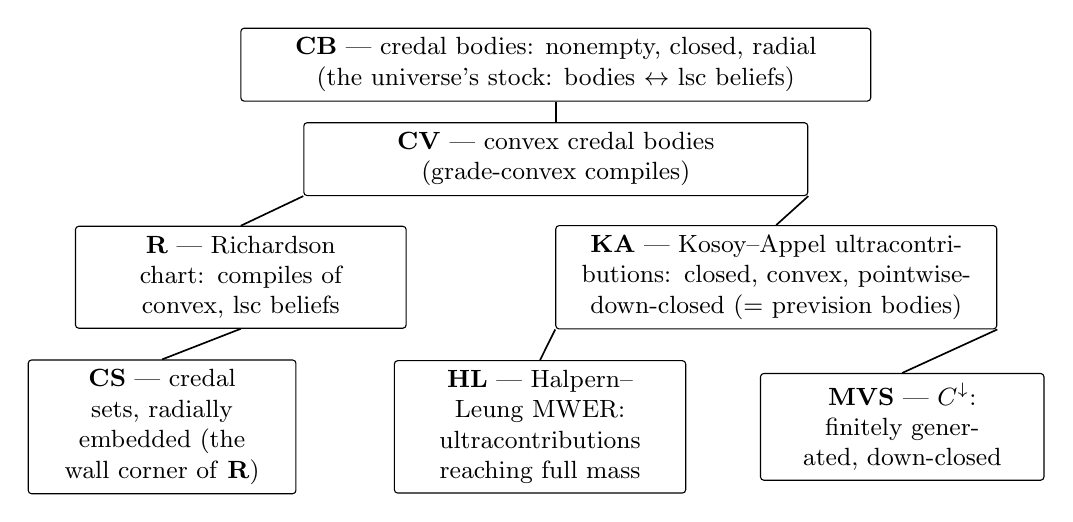
\begin{tikzpicture}[x=1mm,y=1mm,
  cls/.style={draw, rounded corners=1.2pt, align=center,
    font=\small, inner xsep=2mm, inner ysep=1.2mm},
  cover/.style={semithick}]
  \node[cls, minimum width=80mm] (CB) at (0,46)
    {\textbf{CB} --- credal bodies: nonempty, closed, radial\\
     (the universe's stock: bodies $\leftrightarrow$ lsc beliefs)};
  \node[cls, minimum width=64mm] (CV) at (0,34)
    {\textbf{CV} --- convex credal bodies\\ (grade-convex compiles)};
  \node[cls, text width=38mm] (R) at (-40,19)
    {\textbf{R} --- Richardson chart: compiles of convex, lsc
     beliefs};
  \node[cls, text width=52mm] (KA) at (28,19)
    {\textbf{KA} --- Kosoy--Appel ultracontributions: closed, convex,
     pointwise-down-closed ($=$ prevision bodies)};
  \node[cls, text width=30mm] (CS) at (-50,0)
    {\textbf{CS} --- credal sets, radially embedded (the wall corner
     of \textbf{R})};
  \node[cls, text width=33mm] (HL) at (-2,0)
    {\textbf{HL} --- Halpern--Leung MWER: ultracontributions reaching
     full mass};
  \node[cls, text width=32mm] (MVS) at (44,0)
    {\textbf{MVS} --- $C^{\downarrow}$: finitely generated,
     down-closed};
  \draw[cover] (CV.north) -- (CB.south);
  \draw[cover] (R.north) -- (CV.south west);
  \draw[cover] (KA.north) -- (CV.south east);
  \draw[cover] (CS.north) -- (R.south);
  \draw[cover] (HL.north) -- (KA.south west);
  \draw[cover] (MVS.north) -- (KA.south east);
\end{tikzpicture}
\caption{The atlas of credal-body subclasses
(Remark~\ref{rem:su-body-atlas}) as a Hasse diagram, higher $=$
larger. Every edge is a strict inclusion --- placement a
general-carrier theorem, strictness a two-point rational witness ---
and every pair not joined by a path is incomparable, both directions
witnessed over the same two-point outcome space; the receipts are
the modules cited in the remark. The credal-set class enters by
radial embedding, and precise models are its singleton corner.}
\label{fig:su-body-atlas}
\end{figure}

\begin{remark}[The atlas of credal-body subclasses]
\label{rem:su-body-atlas}
The literature's imprecise-probability objects sit inside the credal
bodies as distinguished subclasses, and the inclusions between them
are part of this universe's content --- Figure~\ref{fig:su-body-atlas}
draws the poset. Read through the compile, the same atlas is the
chart of full subcategories of the thin category of beliefs drawn
in \cite{dalrymple26imprecise}, with the explicit transforms
mechanized here. The inclusion spine is
kernel-checked at the \emph{general} carrier --- subprobability
measures over an arbitrary record space, each placement below a
theorem
(\texttt{SuFunctor.Universe.General.CredalPoset},
\texttt{SuFunctor.Universe.General.Richardson}) --- while the
finite-rational stratum remains the reference case for the
\emph{separations}: every strict edge and every
incomparability a two-line rational witness over a two-point
outcome space, and the outer class containing all of them
(\texttt{SuFunctor.Universe.CredalPoset}:
\texttt{house\_includes\_all}).
Two closure notions must be kept apart first: \emph{radiality}
((C3): closed under scaling $\nu \mapsto \lambda\nu$,
$\lambda \in [0,1]$) and \emph{down-closure} in the pointwise order
on measures ($\nu' \le \nu$ setwise implies membership).
Down-closure implies radiality; the converse fails --- a single ray
$[0,1]\cdot\mu$ is radial and, for non-degenerate $\mu$, not
down-closed. With that distinction in hand:
\begin{itemize}
\item \emph{precise models}: the rays $[0,1] \cdot \mu$ --- closed,
  radial, convex; the compiles of the beliefs vanishing at a
  single law (Remark~\ref{rem:su-faces});
\item \emph{credal sets}, in the sense of Cozman's credal-network
  literature \cite{cozman00}: nonempty closed convex sets $M$ of
  \emph{full-mass} laws, entering as the radial closure
  $[0,1] \cdot M$, with $S^{\max} = M$ --- and closedness of the
  radial closure is proved \emph{through the dictionary}: the
  radial embedding of a closed convex full-mass set is the compile
  of its direction wall
  (\texttt{scaleSegment\_eq\_compile\_dirWall}), so the body-side
  regularity is Remark~\ref{rem:su-belief-iso-mechanized}'s
  closedness theorem applied, not a separate argument. A credal set
  enters the universe twice over: as its \emph{wall} --- the
  indicator belief $\chi_M$ of Remark~\ref{rem:su-faces}, the
  possibilistic reading --- and as its \emph{Hausdorff--KL
  embedding} $\mu \mapsto \min_{\nu \in M} \mathrm{KL}(\mu \,\|\,
  \nu)$, the graded reading of the same set: zero exactly on $M$,
  relative-entropy-graded off it --- the set-valued extension of
  the Gibbs chart of the grades paragraph above, with the direction
  of the divergence \emph{forced} rather than chosen: under the
  epistemology's multiplicative-weight update
  \cite{dalrymple26imprecise} (add the expected
  surprisal $E_{\mu}(-\log L)$, renormalize), the wall reading can
  only delete states, the reversed-divergence reading collapses to
  the vacuous belief, while the Hausdorff--KL reading conditions
  each member and charges it the surprisal of its own marginal
  likelihood --- likelihood updating of weighted sets of
  probabilities in the sense of Halpern and Leung \cite{halpern13},
  whose zero set is the maximum-likelihood update of Gilboa and
  Schmeidler \cite{gilboa93} (Dempster conditioning, on
  belief-function credal sets), and whose graded part retains
  exactly the marginal-likelihood record that element-wise
  conditioning \cite{cozman00} forgets (kernel-checked at the
  finite stratum, including the failure of the element-wise square:
  \texttt{SuFunctor.Universe.HausdorffKL});
\item \emph{Richardson's universe} \cite{richardson20}: bodies
  compiled from beliefs both \emph{convex} and
  \emph{lower semicontinuous} --- with the provenance stated
  carefully, because the class is this universe's reading of the
  programme, not a definition of Richardson's: the
  probabilistic-dependency-graph programme never axiomatizes a
  codomain class at all --- it proves convexity of its inconsistency
  measure as a lemma and never mentions semicontinuity --- so the
  reading takes both properties as definitional, assuming them of
  the programme's beliefs. The assumption is verified
  where checkable: the per-edge conditional relative entropies and
  their nonnegative combinations (the inconsistency measure itself)
  are jointly convex and lower semicontinuous, classically; the full
  $\gamma$-weighted scores, which add signed conditional-entropy
  terms, are convex exactly in the programme's own weight regime
  (edge confidence at least $\gamma$ times the structural weight ---
  the programme's convexity analysis states this bound, and outside
  it a two-outcome double-edge graph gives an exact rational
  counterexample). Neither half of the reading is redundant.
  Convexity of the belief is sufficient, not necessary, for
  convexity of the body
  --- $e^{f}$ convex is the exact condition, and on a two-point
  record space the belief $\log(2 - \mu\{a\})$ is strictly concave
  along the simplex while its exponential is affine, a
  kernel-checked witness with its exact rational comparison
  (\texttt{QtslAux.Imprecise.PenaltyCredalIso}). And the lsc half is
  not implied by the convex half: a bounded, two-valued convex
  belief's body can fail to be topologically closed, the failure
  a jump at the simplex boundary --- a convex function is
  automatically continuous on the relative interior, so
  boundary-lsc is exactly what convexity leaves unsecured
  (\texttt{exists\_penaltyConvex\_not\_closed}), and the same
  witness compiles to a body that no convex lsc belief compiles,
  so the two-property class is strictly smaller than the
  convexity-only reading would have been
  (\texttt{exists\_penaltyConvex\_compile\_not\_richardson}). The
  lsc half is thereby the half that makes the class a subclass of
  the credal bodies at all; the convex half is what places it under
  the convex bodies. The
  placement is a general-carrier theorem, exponential-free: additive
  convexity of the belief implies the exact grade-convexity
  criterion by weighted arithmetic--geometric means
  (\texttt{IsRichardsonBody.isConvexCredalBody});
\item the \emph{convex credal bodies}: exactly the compiles of
  beliefs with $e^{f}$ convex --- at the general carrier the
  criterion is carried division-free, as the cross-multiplied
  harmonic form (\texttt{GradeConvex}), with the compile of any
  grade-convex belief a convex body
  (\texttt{convexBody\_compile\_of\_gradeConvex}) --- and the
  subclass on which
  single-shot linear tests --- prevision-shaped functionals, in the
  sense of Goubault-Larrecq's prevision domains
  \cite{goubaultlarrecq07, goubaultlarrecq08} --- are a complete
  instrument, by Fenchel--Moreau duality;
\item \emph{homogeneous ultracontributions} (Kosoy and Appel
  \cite{kosoy20}): nonempty topologically closed \emph{down-closed}
  convex sets of subprobability laws --- inside the convex bodies,
  since down-closure implies radiality
  (\texttt{IsUltra.isConvexCredalBody}, at the general carrier).
  Every prevision-shaped body --- a set cut out by a family of
  one-sided gamble constraints, the hyperspace object of
  Goubault-Larrecq's superlinear-prevision domains --- is an
  ultracontribution at the general carrier
  (\texttt{IsPrevisionBody.isUltra}); on the finite stratum the
  inclusion is an \emph{equality}
  (\texttt{isPrevisionBody\_iff\_isUltra}): one poset node, two
  presentations, infra-Bayesian induction and the domain-theoretic
  prevision school meeting in one theorem --- with the general
  converse Hahn--Banach-shaped, a named successor rather than a
  silent assumption;
\item the $C^{\downarrow}$ \emph{monad} of Mio, Sarkis, and
  Vignudelli \cite{mio20}: nonempty \emph{finitely generated}
  down-closed convex sets --- inside the ultracontributions
  wherever the setwise order of measures is narrowly closed, a
  hypothesis the mechanization carries explicitly rather than
  silently: hulls of finite generating families are compact for
  \emph{any} carrier (the weight-simplex route), so finite
  generation implies closedness under exactly that named
  order-closedness (\texttt{isClosed\_ptwiseDownHull},
  \texttt{IsMVS.isUltra}) --- free at the finite stratum,
  dischargeable on metrizable carriers, and not free in general;
\item the semantics of Halpern and Leung's minimax weighted
  expected regret \cite{halpern13}: topologically closed
  down-closed convex sets of subprobability laws \emph{each
  containing at least one full-mass law} --- the ultracontributions
  whose maximal slice reaches the probability face, which is
  condition-for-condition Kosoy and Appel's \emph{homogeneous
  ultradistribution} --- although neither cites the other --- the
  subprobability encoding being Halpern
  and Leung's own.
\end{itemize}
Every class above is a class of credal bodies, so the present
universe includes them all; the chain $C^{\downarrow} \subseteq
\text{ultracontributions} \subseteq \text{convex bodies} \subseteq
\text{credal bodies}$ is strict at every step already over a
two-point outcome space; the credal-set and precise classes enter
through radial closure rather than down-closure (their radial
closures are not down-closed in general); and the regularity that
closes the whole atlas at the top is closedness alone --- the lsc
face of the compile, with no convexity anywhere in the outer class.
\end{remark}

\subsection{Envelopes: Previsions and the Degenerate Faces}

From either presentation the operators of record are the envelope
expectations, split across the slice exactly as
Remark~\ref{rem:su-maximal-slice} forces.

\begin{definition}[Lower and upper previsions of a credal body]
\label{def:su-previsions}
Adopt the standing structure of
Definition~\ref{def:su-credal-denotation}. A \emph{gamble} is a
Borel function $h \colon \mathcal{X} \to (-\infty, +\infty]$ bounded
below; its expectation under $\nu \in \Delta_{\le 1}(\mathcal{X})$
is well-defined in $(-\infty, +\infty]$. For a credal body $S$
with radially maximal slice $S^{\max}$, the \emph{lower prevision}
and \emph{upper prevision} of $h$ under $S$ are
\[
  \underline{E}(h) \;:=\; \inf_{\nu \in S^{\max}} E_\nu(h), \qquad
  \overline{E}(h) \;:=\; \sup_{\nu \in S} E_\nu(h),
\]
with $\inf \varnothing = +\infty$ (so the bottom credal body ---
the nonempty set $\{0\}$, whose maximal slice is empty --- has
vacuously infinite lower previsions). For events we write
$\underline{P}(A) := \underline{E}(\mathbf{1}_A)$ and
$\overline{P}(A) := \overline{E}(\mathbf{1}_A)$. The lower prevision
must read the maximal slice
(Remark~\ref{rem:su-maximal-slice}); the upper prevision is defined
over all of $S$, and for nonnegative gambles and $S \ne \{0\}$ the
suprema over the two index sets agree (the sets themselves do not). Full boundedness is required exactly where the two envelopes
are \emph{combined} --- imprecision gaps and the attitude blends
below --- since those expressions are undefined when an envelope is
infinite.
\end{definition}

A specification's probability operator
$\mathsf{P}_{\ge p}[\varphi]$ denotes the lower probability
$\underline{P}(\varphi) \ge p$ --- certification pessimism, always.
Three faces of one object, and the flat operator survives as a face
rather than a casualty:

\begin{remark}[The degenerate faces, stated exactly]
\label{rem:su-faces}
The two flat verdict operators survive inside the credal stack as
compiles of indicator-type beliefs.
\begin{enumerate}
\item \emph{Precise face.} For $\mu_0 \in \Delta(\mathcal{X})$, the
  belief vanishing at $\mu_0$ and infinite elsewhere is lower
  semicontinuous, and its compile is the single ray
  $S = [0,1] \cdot \mu_0$ with $S^{\max} = \{\mu_0\}$. The maximal
  slice is the singleton: both envelope operators then read $\mu_0$
  alone, and the denotation is an ordinary (precise) probability
  model. It is the slice, not $S$ itself, that is a singleton --- a
  credal body is never a one-point set except at bottom.
\item \emph{Possibilistic face.} Let $B \subseteq \mathcal{X}$ be a
  closed set of allowed records and
  $D_B := \{\mu \in \Delta(\mathcal{X}) : \mu(B) = 1\}$ the
  distributions supported on $B$ --- convex, weakly closed, the
  closed convex hull of the point masses on $B$. The possibilistic
  belief ($0$ on $D_B$, $\infty$ elsewhere) is convex lower
  semicontinuous, and on this face upper
  probabilities are Boolean:
  $\overline{P}(A) = 1$ if $A \cap B \neq \varnothing$ and $0$
  otherwise, so $\overline{P}(\mathrm{bad}) = 0$ \emph{is} the
  behavioural verdict ``bad is forbidden.'' The zero-set is all
  of $D_B$, not merely the point masses --- with convexity no
  longer a membership condition, the point-masses-only belief is
  also a lawful member, whose body is the union of the
  rays through the point masses; when $B$ contains at least two
  points that body is nonconvex and the belief sits strictly above
  $\chi_{D_B}$ in the order (for empty or singleton $B$ the two
  coincide), and the face that reproduces classical
  possibility theory is $D_B$.
\end{enumerate}
The classical imprecise-probability world embeds by the same device
one level up: an ordinary credal set $M \subseteq \Delta(\mathcal{X})$
(nonempty, convex, closed, all elements of full mass) corresponds to
the indicator belief $\chi_M$, whose compile is the radial closure
of $M$ with $S^{\max} = M$ --- the atlas of
Remark~\ref{rem:su-body-atlas} places this and its relatives.
Strictly graded beliefs --- the soft,
dependency-graph-typed models --- are exactly the credal bodies
whose maximal slices contain submass measures.
\end{remark}

\begin{remark}[The envelope calculus: the ray and its maximal slice]
\label{rem:su-envelope-reconciliation}
A precise law $\mu$ denotes as its ray $[0,1]\cdot\mu$ --- the
credal body, its entry into the universe --- and the wiring stratum
computes with the ray's \emph{radially maximal slice}, which for
$\mu \neq 0$ is exactly the singleton $\{\mu\}$
(\texttt{maxSlice\_rayC}). That the device is faithful to the
denotation is kernel-checked, hypotheses included, in module
\texttt{SuFunctor.Adequacy.Envelope}: the two verdict readings
agree kind by kind --- a lower-kind (slice-reading) verdict against
the ray is the verdict at $\mu$
(\texttt{satCredal\_lower\_rayC}), and an upper-kind (whole-set)
verdict agrees between ray and slice for every
\emph{down-closed} constraint (\texttt{DownClosed}; event upper
bounds qualify, with no hypothesis on $\mu$). The boundary is part
of the theorem, not a footnote: at $\mu = 0$ the slice is
\emph{empty} --- the bottom credal body, per
Remark~\ref{rem:su-maximal-slice} --- and ray and slice
agree as raw constraints \emph{only} there
(\texttt{rayC\_eq\_singletonC\_iff}): divergence is governed by
$\mu \neq 0$, not by submass. Mixing the two readers is
refuted as a theorem, not discouraged as a convention: reading a
lower-kind atom with the whole-set reader refuses every positive
threshold, for every $\mu$, the ray's zero element being the
universal refuter (\texttt{not\_satCredal\_upper\_rayC\_geC}). For
the squares' consumers the hypothesis discharges for free: a
compiled stochastic frame's law has mass one, hence is nonzero. The
set-valued extension is kernel-checked in module
\texttt{SuFunctor.Adequacy.EnvelopeUnion}. For a \emph{family} of
laws the set-valued presentation is the union of the members' rays:
radial and, for a closed family, itself a credal body, though
in general \emph{not convex}. Whether the closed convex hull is
taken is a modelling fact, not a convention: an adversary with
strategy access over the family can \emph{mix}, and for such faces
the hull is the achievable set --- the correct denotation --- while
for a parameter fixed once and unknown the bare union is the correct
denotation, and taking the hull would add mixtures the family cannot
realize. The
slice of the union always sits inside the family
(\texttt{maxSlice\_unionRays\_subset}, hypothesis-free), and for a
family of equal nonzero mass the slice is exactly the family
(\texttt{maxSlice\_unionRays}), equal mass being spent on
cross-ray domination. Fixtures witness the hypothesis's necessity:
a \emph{nonempty} all-zero family collapses its union to the bottom
object with an empty slice, exactly as the single-ray boundary
predicts, and the empty family yields the empty union, which sits
below even bottom.
\end{remark}

\subsection{Gluing: The Imprecise Extension Problem}

A System's
mechanisms hand the semantics \emph{local} credal data --- interval
kernels, rate intervals, disturbance sets --- on finite windows; the
denotation must be a global object on records whose restrictions
reproduce the local data. This is the Kolmogorov extension problem,
transposed, and its imprecise answer stratifies along the record direction:

\begin{itemize}
\item \emph{Existence and exactness, kernel-presented case.} When
  local data arrive as compact credal sets of transition kernels in
  the record direction --- the shape discrete-time mechanism
  presentation produces --- the glue exists with no topological
  hypotheses beyond that compactness, is computed by iterated
  marginal extension, and reproduces the local models on the nose:
  the Marginal Extension Theorem of de Cooman and Hermans
  \cite{cooman08} for imprecise probability trees, with backwards
  recursion as its computational face. The on-the-nose verdict
  carries its scope wherever this book leans on it: discrete-time
  record posets, finite or discrete state, compact credal local
  sets, and Williams-coherent globals. Continuous-state and
  continuous-time mechanisms hand the semantics local data through
  their own doctrine presentations; their extension theory is named
  debt in \autoref{sec:su-receipts}, not a corollary of the
  kernel case.
\item \emph{Uniqueness fails --- by design.} Many coherent global
  models share the same finite-window restrictions. The canonical
  choice is a universal property, not an isomorphism: the
  \emph{natural extension} --- the least-committal coherent glue,
  pointwise-smallest lower expectation at
  Definition~\ref{def:su-natural-extension}'s stated scope, largest
  compatible set of models (convex as a theorem, not by fiat; see the
  definition). The slogan this
  makes precise carries through everything in
  \autoref{sec:su-composition}: the model constrains the
  distributions; it does not select one.
\item \emph{Beyond the record direction, the flavour of coherence is
  a real choice.} For parallel cover shapes on infinite spaces,
  Walley-coherent independent products can fail to exist (Miranda
  and Zaffalon \cite{miranda-zaffalon-2015-independent-products});
  adopting Williams coherence repairs existence (De Bock's
  independent natural extension), and this universe adopts Williams
  coherence as its default --- a genuine doctrinal selection,
  recorded here, with no consequence at finite
  state where the flavours coincide.
\end{itemize}

\begin{definition}[Coherent lower prevision; natural extension]
\label{def:su-natural-extension}
Let $L$ be the linear space of bounded Borel gambles on
$\mathcal{X}$. A functional
$\underline{P} \colon L \to \mathbb{R}$ is a \emph{coherent lower
prevision} when, for all $h, g \in L$ and real $\lambda \ge 0$:
\begin{itemize}
\item[(W1)] $\underline{P}(h) \ge \inf h$;
\item[(W2)] $\underline{P}(\lambda h) = \lambda\,\underline{P}(h)$;
\item[(W3)] $\underline{P}(h + g) \ge \underline{P}(h) +
  \underline{P}(g)$.
\end{itemize}
Its conjugate upper prevision is
$\overline{P}(h) := -\underline{P}(-h)$. An \emph{assessment} is a
pair $(K, c)$ with $K \subseteq L$ and $c \colon K \to \mathbb{R}$
assigning claimed lower bounds --- the local data a System's
mechanisms hand the semantics. Its \emph{compatible set} is
\[
  M(K, c) \;:=\;
  \bigl\{P \in \Delta(\mathcal{X}) :
    E_P(h) \ge c(h) \text{ for all } h \in K\bigr\},
\]
and $(K,c)$ \emph{avoids sure loss} when $M(K,c) \neq \varnothing$.
The \emph{natural extension} of an assessment avoiding sure loss is
$\underline{E}_{K,c}(h) := \inf_{P \in M(K,c)} E_P(h)$; equivalently
--- exactly, for finite $\mathcal{X}$, by linear-programming duality
--- it is computed by finite positive combinations of assessment
deficits. Universal property, with its scope stated in the same
breath: $\underline{E}_{K,c}$ is a coherent lower prevision
dominating the assessment, and at finite $\mathcal{X}$ it is the
pointwise-smallest such functional outright --- at infinite
$\mathcal{X}$ the countably additive envelope displayed here is
least among the \emph{countably-additive-envelope} lower previsions
dominating the assessment, the classical unrestricted minimum being
represented by finitely additive probabilities, per the agreement
scope below; dually $M(K,c)$ is the largest compatible \emph{set} of
models outright --- the comprehension takes every compatible model,
and no convexity clause appears. Its convexity is a \emph{theorem}:
each constraint $E_P(h) \ge c(h)$ is affine in $P$, so the compatible
set is an intersection of half-spaces with the simplex (and closed
whenever the assessment's gambles are continuous --- expectation
against a merely Borel gamble is not a weakly continuous functional,
so closedness is a hypothesis at the standing generality, not a
freebie).
Least-committal lower prevision and largest compatible set are the
same universal property read on the two sides of the envelope
correspondence: the natural extension adds no commitment beyond what
the assessments force.
\end{definition}

\begin{remark}[Mechanization status of the envelope package; the
partiality departures]
\label{rem:su-envelope-theorem}
Kernel-checked in this repository, at the finite-rational stratum
(module \texttt{QtslAux.Imprecise.Credal}): the envelope face of the
coherence axioms over credal sets presented as finite families ---
attainment of both envelopes, superadditivity of the lower and
subadditivity of the upper, positive homogeneity, and monotonicity.
Kernel-checked at the general carrier --- an arbitrary measurable
record space, countably additive models, bounded measurable gambles
under the Bochner expectation (module
\texttt{QtslAux.Imprecise.NaturalExtensionGeneral}): envelopes of
arbitrary nonempty families of probability measures as coherent
lower previsions (no convexity or closure of the family consumed);
the compatible set, avoidance of sure loss, and the natural
extension as the envelope over the compatible set, with the
universal property at exactly the stated scope of
Definition~\ref{def:su-natural-extension} --- least among the
countably-additive-envelope lower previsions dominating the
assessment (\texttt{natExtG\_le\_lowerEnvG}), the dominating-family
hypothesis itself certifying avoidance of sure loss
(\texttt{avoidsSureLossG\_of\_dominating}), so no separate
feasibility hypothesis enters --- together with the
largest-credal-set dual, convexity of the compatible set in mixture
form, and the definition's closedness parenthetical as a theorem:
the compatible set is narrowly closed whenever the assessment's
gambles are continuous. One storey up, where denotations are credal
bodies rather than subsets of $\Delta(\mathcal{X})$
(section~\ref{sec:su-hyperspace}), the same universal property is
available with no convex vocabulary at all: an assessment's
constraints have walls, the natural extension is the \emph{join of
those walls} in the pointwise order, and its body is the
\emph{largest compatible body} --- the radial compile of the largest
compatible set of laws. For assessment-shaped (gamble-bound)
constraints this body is convex by the affinity theorem above, read
through the compile; for structured constraints the same join is the
right object and is genuinely non-convex --- an independence
assertion's body is a credal body and not a convex one (the
kernel-checked witness of the epistemic-states module: the diagonal
mixture of two deterministic independencies is perfectly
correlated), which is why citizenship in this universe is lower
semicontinuity and never a shape axiom. The distinction is invisible
at the lower-prevision stratum by construction --- expectation is
affine in the model, so a body and its closed convex hull have the
same lower envelope on every gamble --- and taking the hull is
exactly \emph{demonic-choice} semantics: the correct reading where
an adversary may mix admitted laws, and a canonical representative
rather than a definitional ingredient everywhere else. The classical
``largest credal set'' formulation is thus recovered, not
presupposed: it is the demonic representative of the body-level
universal property. The point-free face of envelope coherence
--- the superlinear class closed under lower envelopes, over
gambles in sublevel presentation with the Choquet pairing --- is
kernel-checked in the point-free tower
(\texttt{Pointfree.Prevision}). Kernel-checked at the finite
stratum, where the claims themselves are finite (finite record
spaces, real scalars; module
\texttt{QtslAux.Imprecise.NaturalExtension}): the
sup-of-deficit-combinations display as exact
linear-programming duality, alongside the sure-loss alternative;
and the finite
envelope theorem --- every coherent lower prevision on a finite
record space is the lower envelope of its credal set, in both the
attained form and the envelope display --- the separating engine,
one invocation powering the package, being sublinear Hahn--Banach
extension. At infinite $\mathcal{X}$ the classical envelope theorem
represents coherent lower previsions by \emph{finitely additive}
probabilities; the countably additive envelope is this book's
definition, and the identification of the two representations is
used only inside the finite-state agreement domain --- beyond it,
named debt. \emph{Partiality departures, computed}: over the
maximal slice of a submass-admitting credal body, (W2) and
(W3) persist verbatim, but (W1) weakens to
$\underline{E}(h) \ge \min(\inf h, 0)$ and constant-additivity fails
by exactly the leaked mass --- deliberate, and why the axiomatic
notion is stated on the full-mass stratum, where the classical
theory is recovered exactly. The leak-aware safe-side accounting is
kernel-checked in this repository (module \texttt{QtslAux.LeakAware}): the mass-split union bound,
the per-element and envelope forms of the safe-side subtraction (for
a partial model
$P(\mathrm{safe}) = P(1) - P(\mathrm{bad})$, not
$1 - P(\mathrm{bad})$), the full-mass recovery of the familiar
$1 - V(x_0)$ floor, and a total-leak counterexample certifying that
the naive floor is \emph{unsound} for submass models.
\end{remark}

\subsection{Agreement, and the Attitude Operator}

\paragraph{Agreement.} The scope first: the
agreement theorems of this paragraph are proven for finite state
spaces in discrete time; their continuous-state and continuous-time
lifts are named debt, and certificate soundness (which needs only a
per-element argument, \autoref{sec:su-checker-anchor}) does not
wait on them. Within that
scope, the global object admits three constructions that are not
obviously equal: the game-theoretic upper expectation of Shafer and
Vovk \cite{shafervovk19} (an infimum over hedging supermartingales),
the axiomatic
most-conservative extension of T'Joens, De Bock, and de Cooman
\cite{tjoens20}, and the measure-theoretic envelope over all
compatible precise processes. The agreement theorems state that the
three coincide on monotone limits of finitary gambles and on
bounded-below Borel path functionals --- and the specification
logic's query class sits inside that domain by construction. This
book works with the game-theoretic presentation; the reason is an
adapter fact, stated with the rest of the adapter material where it
belongs (\autoref{sec:su-checker-anchor}): certificate rows
enter the defining infimum \emph{definitionally}.

\paragraph{The attitude operator.} Certification is pessimism
($\underline{E}$ of goodness-valued functionals; equivalently the
$\overline{E}$ of the loss). Design exploration wants the other end
too, and occasionally a weighted blend --- Hurwicz's
optimism--pessimism criterion \cite{hurwicz51}, transposed: for $\alpha \in [0,1]$
and a \emph{bounded} path functional $h$,
$H_\alpha(h) = \alpha\, \overline{E}(h) + (1-\alpha)\,
\underline{E}(h)$, stated for goodness polarity so $H_1$ is pure
best-case optimism and never a guarantee quantity. The endpoints
compose along records for the natural-extension denotations
mechanism presentation produces (the marginal-extension tower
property); interior $\alpha$ does not, and the failure is an
exact-rational fact --- a two-stage interval-kernel chain realizes
root-blend $\tfrac{15}{32}$ against stagewise-blend
$\tfrac{14}{32}$, and a second instance reverses the sign, so
composed interior-$\alpha$ scores are neither sound bounds nor
reliable estimates. The design consequence is a restriction the
grammar adopts wherever the operator appears: $H_\alpha$ is a
\emph{root-only} query operator with no congruence rule, evaluated
by the two passes that do compose and mixed once at the root, and
any verdict at $\alpha > 0$ renders as a design score, never as a
guarantee. The structural derivation sits beside the
kernel-checked counterexample: an interior blend mixes a
refinement-monotone and a refinement-antitone quantity, so it is
not monotone in the universe's refinement order and therefore not
an entailment-shaped operator at all --- the root-only restriction
is the order speaking.
Attitude lives in the query. Systems carry none.
\section{The Hyperspace Storey}
\label{sec:su-hyperspace}

The universe of \autoref{sec:su-denotation} is a space of
functions with a pointwise order. Everything the specification
logic will ask of the universe --- connectives, entailment under a
context, case analysis, and the composition calculus's fibres ---
lives one storey up, on \emph{sets} of denotations, and this
section fixes that storey: the hyperspace, the passage from heights
to bodies, and the two facts that organize all later use --- from
this storey up the order of the universe is inclusion, and Systems
enter as singleton elements.

\paragraph{From heights to bodies.} A belief $\sigma$ on the
probability face compiles to its \emph{body}: the closed radial
subset of the subprobability carrier admitting each law $\mu$ at
every scale up to its grade,
$S(\sigma) = \{\gamma\mu : \gamma \le e^{-\sigma(\mu)}\}$ ---
Definition~\ref{def:su-belief}'s compile, kernel-checked
at the general carrier, with the finite stratum carrying both exact
presentations
(Remark~\ref{rem:su-belief-iso-mechanized}). Under the compile the
pointwise order on the radial stock becomes inclusion of bodies,
belief addition becomes the fibrewise grade product, and the height
calculus of \autoref{sec:su-denotation} is available, on that
stock, as a calculus of closed radial sets: one structure with two
interchangeable presentations, heights for arithmetic, bodies for
topology. The
\emph{hyperspace} of the storey is the space of closed subsets of
the subprobability carrier under the Fell topology of
\autoref{sec:su-carrier} --- compact with no hypotheses on the
carrier, and the home of every body, since bodies are closed by
definition. And the storeys compose: the record storey already did
its work in the Fell topology, so a window's record space arrives
\emph{compact} metrizable (\autoref{sec:su-carrier}), and the
subprobability carrier over it is compact Hausdorff (on a compact
carrier the weak and vague readings coincide, and the carrier is
weak-star closed in the unit ball --- Alaoglu, standard); on the
finite stratum it is the simplex, compact on sight. On a compact
Hausdorff carrier Fell and Vietoris are \emph{one} hyperspace
topology --- the Fell form agrees with the nonempty-compacts
Vietoris presentation, kernel-checked at exactly those hypotheses
(\texttt{fell\_eq\_vietoris}) --- and the nonempty bodies are
compact, so that presentation is the exact stratum's home for the
class machinery below. The machinery itself no longer needs the
compactness mediation: crescents, their two faces, local
closedness, the constructible algebra, and the judgment transport
are kernel-checked at the general carrier directly, over the Fell
hyperspace of an arbitrary topological measurable record space
(\texttt{SuFunctor.Universe.General.CrescentStratum} --- both
crescent faces ride the hit-open subbasis Fell and Vietoris share:
the containment face closed because its complement is a hit of an
open, the escape faces hit-opens outright), with the
compact/Vietoris presentation surviving as the exact-collapse
special case. For a carrier that arrives noncompact, the
one-point-compactification mediator,
$\mathrm{CL}(Y) \cong \{B \in \mathcal{K}(Y^{+}) : \infty \in B\}$
(Remark~\ref{rem:su-carrier-mechanized}), still carries the Fell
form into the compact presentation where the exact stratum wants
it.

\paragraph{The order at this storey is inclusion.} On bodies the
universe's order reads $S(f) \subseteq S(h)$ iff $f \ge h$
(Definition~\ref{def:su-belief}), and from here up ---
bodies in classes, classes in classes, fibres over the wiring base
--- every comparison this universe supports \emph{is} an inclusion.
This is the form of the order the specification logic's judgments
will consume when later chapters interpret the logic here: not a
new relation at each storey, but one order --- pointwise on
beliefs, exchanged by the compile with inclusion at the
hyperspace, read off the fibre carriers of the composition construction
unchanged (\autoref{sec:su-composition}).

\paragraph{Systems are singleton elements.} A System enters the
storey as the singleton $\{S(\sigma)\}$ of its body --- an
\emph{ideal point} of the hyperspace. The name records a theorem,
not a convention --- singletons are not spec-definable (no formula
of the spec syntax denotes a one-point class:
\texttt{singletons\_not\_definable}, with its upper-open companion),
so a precise refinement can never be pinned by Spec syntax and
selection data is certificate content, never formula content. And
the embedding leaves no residue: membership of a body in a class is
inclusion of its singleton in the class --- the fibre order of
\autoref{sec:su-composition}, at one window
(\texttt{idealPoint\_le\_iff}) --- so ``Systems are singleton
elements of the hyperspace'' is the exact sense in which one order
serves every boundary: body above body, singleton inside class,
class inside class.

\section{The Fibre of Specs: Constructible Classes in the
Hyperspace}
\label{sec:su-classes}

A Spec needs more than one body at a time. The logic conjoins
Specs, disjoins them, asks whether one entails another under a
context, and wires the Systems they govern into larger Systems.
Each of those acts consumes classes of bodies rather than single
bodies, and the classes must survive all of them at once. This
section fixes the classes. The atoms of the stratum denote
\emph{crescents}: one closed containment face, cut by finitely many
open escape faces. Compound Specs denote finite unions of
crescents, which live in the \emph{finitary constructible algebra}
of the hyperspace. Entailment denotes inclusion of classes, and a
finite blocking criterion decides it. Every demand the logic places
on this structure is discharged as a theorem, and the section ends
where the theorems currently end: at the algebra's boundary, where
the attitude classes of \autoref{sec:su-denotation} provably live
outside it, and where a completion question stands open.

What a logic may ask of its classes was settled long before this
book. Categorical logic, since Lawvere, reads predicates as objects
of fibres over a base of contexts and states what each connective
demands \cite{lawvere69,lawvere70}. Substitution must act
functorially along the maps of the base. Entailment must be the
order of each fibre, and posets suffice for a proof-irrelevant
sequent logic. Conjunction and disjunction must denote fibrewise
lattice structure, preserved by reindexing, with the distributive
law available to the context-carrying elimination rules.
Quantifiers, where a logic has them, must be adjoints to
substitution, subject to Frobenius reciprocity and the
Beck--Chevalley condition. Jacobs gives the systematic dictionary
between fragments of logic and the fibred structure each fragment
demands \cite{jacobs99}; Pitts surveys the same territory
\cite{pitts00}; Melli\`es and Zeilberger reconstruct Lawvere's
setting bifibrationally \cite{mellies16}. The Spec connectives
speak the \emph{coherent} fragment: finite conjunction, finite
disjunction, top and bottom; no negation, no implication, no
quantifier former. Its categorical model theory is classical
\cite{makkaireyes77}, and the match is designed rather than
residual. Coherent sequents are the sequents the blocking criterion
below decides with finite certificate data --- domination rows,
selections, choice bytes --- and the same fragment, in its
implicational dress, is the one the Geolog engine's chase evaluates
(\autoref{ch:geolog-reference}). Certifiability chose the fragment;
the tradition then says what the fibre owes.

The debts are paid in order. Atoms and their classes come first,
together with the polarity discipline that replaces any
monotonicity intuition a reader might import. The disjunction
theorem then removes the one degree of freedom an interpreter might
believe remains. The blocking criterion decides entailment. Three
refusals close the account: negation, refused by the carrier;
quantifiers, declined at this stratum while the genuine adjoint
lives one storey down; and attitudes, refused by a theorem. Beneath
the atoms, the graded layer explains why graded judgments demand
no graded classes, and a final subsection states the completion
question the refusals leave open. On evidence, one standing note:
the coherence claims of this section cite receipts from multiple
proof-checking kernels (Lean~4, SafeVerify, and \texttt{nanoda};
\autoref{sec:su-receipts} states what each checks), the receipts
are re-runnable, and the claims that do not yet have them are
labelled rather than blended in. This section is where that
discipline proved its worth --- the design-record instance after
Theorem~\ref{thm:su-vee-forcing} tells the story.

\subsection{Atoms: Crescents}

\begin{definition}[Spec atom, and its crescent]
\label{def:su-crescent}
A \emph{spec atom} is a pair $(u, \mathcal{D})$: a \emph{safety
face} $u$, one member of the universe, the atom's floor; and a
finite \emph{liveness set} $\mathcal{D}$ of members, its escape
demands. The atom's class in the hyperspace is its \emph{crescent},
\[
  \mathrm{cres}(u, \mathcal{D}) \;=\;
  \bigl\{K \;\bigm|\; K \subseteq S(u)\bigr\} \;\cap\;
  \bigcap_{v \in \mathcal{D}}
  \bigl\{K \;\bigm|\; K \cap S(v)^{\complement} \neq
  \varnothing\bigr\},
\]
the bodies contained in the safety face's body that escape every
liveness demand's body. The kernel form is
\texttt{SuFunctor.Universe.crescentClass}.
\end{definition}

The two kinds of face quantify in opposite directions, and the
opposition is the atom's content. The containment face demands that
\emph{every} admitted law stay within the floor's body; it is the
safety half of the atom, and the pessimistic pass of
\autoref{sec:su-denotation} discharges it, by domination against
the worst case. Each escape face demands that \emph{some} admitted
law leave the demand's body; it is a liveness conjunct, and the
optimistic pass discharges it, by a witness at the best case. One
atom thus couples a $\forall$-polarized face with finitely many
$\exists$-polarized ones. This is the liveness repair of
\autoref{sec:su-denotation} at the right altitude, and the leak
asymmetry established there governs how partiality counts on each
face.

Topologically, a crescent is one Vietoris-closed containment face
cut by finitely many lower-open escape faces, hence a
\emph{locally closed} subset of the hyperspace
(\texttt{isLocallyClosed\_crescentClass}, in the locally-closed
layer at the general carrier). The shape is kindred to the
hit-and-miss generators of \autoref{sec:su-carrier} --- one closed
demand, finitely many open ones, the cover-modality geometry ---
though the two families are not one: the capacity generators hit
basis opens and miss compact closures, while a crescent's closed
face is a containment. The kinship is what matters. The spec
logic's atoms, the carrier's determination principle, and the
checker's test regions speak one geometry, at two floors of the
same tower.

The transports between an atom's presentation and its class are
exact: a body lies in the crescent with empty liveness set
precisely when its belief dominates $u$ in the universe's order,
and inclusion between safety-only crescents reverses the pointwise
order on their floors. The kernel forms are
\texttt{compileNC\_mem\_crescentClass\_iff} and
\texttt{compile\_subset\_compile\_iff}.

\paragraph{Graded reach-avoid: the atoms, in control-theoretic
dress.} The atoms are a familiar object of control theory wearing
graded clothing. Call a spec atom with one \emph{genuine} liveness
demand --- liveness set $\{\ell, \top\}$, the properness mark
carried along structurally --- a \emph{graded reach-avoid} atom.
Its judgment demands that the system dominate the safety floor $u$
(graded avoidance: the floor prices every admitted law rather than
merely forbidding a region) and dip under the mark $\ell$ (graded
reach: some admitted law strictly undercuts the demanded
bar); the kernel form is
\texttt{mem\_modelClass\_reachAvoid\_iff}. With wall data on both
faces --- a crisp safe set $S$ and a crisp target $T$ --- the
judgment becomes literally the classical possibilistic reach-avoid
demand, \emph{exclude $S^{\complement}$, keep some state of $T$
possible} (\texttt{coupledSat\_crispRA\_iff}), the specification
studied as a decision problem since \cite{summerslygeros10} and
still the benchmark object of certificate-based stochastic
verification \cite{xue25,cao25}. The generalization is strict
already over a one-point carrier, and at the algebra level rather
than atom by atom: no finite $\vee/\wedge$ combination of crisp
reach-avoid classes separates the constant systems $1$ and $0$ ---
every wall admits both or excludes both --- while a graded floor
does (\texttt{exists\_genClosure\_reachAvoid\_not\_crispGenerated}).
The stratum is then \emph{exactly} the completion of graded
reach-avoid under the calculus's two connectives: a class is
constructible if and only if it is a finite disjunction of finite
conjunctions of graded reach-avoid atoms, kernel-checked at both
strata (\texttt{genClosure\_reachAvoid\_iff\_exists\_specDnf} on an
arbitrary carrier;
\texttt{genClosure\_reachAvoidCres\_iff\_exists\_specDnf} in the
hyperspace, with constructibility of the generated algebra as
\texttt{isConstructibleUnion\_of\_genClosure\_reachAvoidCrescentsLsc}).
The decomposition inside a single atom is conjunctive, exactly: a
liveness \emph{set} is the intersection of the singleton-liveness
atoms sharing its floor
(\texttt{modelClass\_eq\_iInter\_reachAvoid},
\texttt{crescentClass\_eq\_iInter\_reachAvoid}), and the
disjunctive reading is refuted outright --- one unsatisfiable
demand empties an atom but not the union of its singletons
(\texttt{exists\_modelClass\_ne\_iUnion\_reachAvoid}). Disjunction
of liveness demands, for its part, never needs the class level at
all: within one atom it is mark-join (\texttt{dip\_sup\_iff}), so
the $\vee$ the completion spends is spent entirely on unions of
classes. Two boundary readings earn the ``exactly.'' The empty
disjunction is generated --- the false Spec, the empty class ---
while the empty conjunction is deliberately not: no constructible
class is trivially true, because every presented atom carries the
properness demand (Remark~\ref{rem:su-presupposition-fork}), and
that same mark is what closes the completion using \emph{binary}
conjunction alone, since every liveness set is nonempty and its
intersection is anchored at the atom's own $\top$-mark. For a
reader arriving from the reach-avoid literature the translation
reads: a Spec of this logic is a finite monotone combination of
reach-avoid demands whose avoidance is priced rather than binary
and whose reach is a strict undercut of a graded bar --- and the
wall fragment (\autoref{sec:su-checker-anchor}) is the crisp
sublanguage through which checked verdicts embed.

\subsection{Classes: the Constructible Algebra}

\begin{definition}[Spec class, and the constructible sets]
\label{def:su-constructible}
The \emph{spec class} of a compound Spec in disjunctive normal
form --- a finite family of atoms $(u_i, \mathcal{D}_i)_{i < n}$
--- is the union of its disjuncts' crescents,
$\mathrm{dnf}\bigl((u_i, \mathcal{D}_i)_i\bigr) = \bigcup_{i<n}
\mathrm{cres}(u_i, \mathcal{D}_i)$. A subset of the hyperspace is
\emph{constructible}, in the finitary sense, when it is a finite
union of locally closed sets
(\texttt{SuFunctor.Universe.IsConstructibleUnion}). The classes of
the stratum are the constructible sets.
\end{definition}

Two boundaries in that definition are deliberate. The notion is
finitary rather than spectral, and the mechanization defines it
directly instead of reusing a library notion: on a connected
compact Hausdorff hyperspace the spectral-space constructible
algebra, generated by compact open sets, degenerates to the
trivial one, while the finitary algebra is the one the spec syntax
generates. And the family is closed under the operations the
calculus performs: finite unions by definition, finite
intersections because crescents intersect to crescents
(\texttt{crescentClass\_inter\_crescentClass}) and intersection
distributes over union by the powerset frame law
(\texttt{inter\_dnfClass\_append}). Top and bottom are the trivial
atom's class and the empty disjunction. Systems enter the stratum
as the ideal points of \autoref{sec:su-hyperspace}: the singleton
class $\{S(\sigma)\}$ of a System's body, spec-undefinable, with
membership read as inclusion.

What makes this algebra \emph{the} fibre, rather than one
candidate among several, is transport. The composition calculus of
\autoref{sec:su-composition} reindexes classes along wirings, and
the transport dictionary makes reindexing \emph{preimage} at the
body level (\texttt{compile\_pullPen}). Preimage respects both
kinds of face --- the pullback of a pointwise join is the join of
the pullbacks, so atom-level transport commutes with atom
conjunction definitionally --- and distributes over the
constructible unions (\texttt{transportClass\_union}), which, for
subobject fibres, is the coherent-category axiom that finite
unions be pullback-stable. So the fibres are posets under
inclusion, the one order of the universe from the hyperspace
storey up; the connectives denote fibrewise lattice structure; and
reindexing preserves it by variance rather than by axiom. The
adjudicated boundary of the transport claim --- atom-level
transport against image transport, exact along surjections,
genuinely divergent off them --- is
Remark~\ref{rem:su-transport-citizenship}, and the double
Grothendieck assembly of \autoref{sec:su-composition} packages the
whole, every obligation kernel-checked, with the window-indexed
families of these classes as its fibre data. The definite article
is earned on two sides: this is the least family that contains the
atoms and holds the connectives, and no larger family currently
carries the assembly's kernel-checked functoriality. Whether a
larger one can is the closing subsection's question.

\subsection{Polarity, not Monotonicity}

Entailment denotes inclusion, and inclusion is an order; a reader
may therefore expect the classes to sit monotonically in the
universe's \emph{other} order, refinement --- every class an
up-set or a down-set of better-and-worse systems. They do not, and
the failure is structural. A containment face is downward closed:
shrink a body inside the floor and it stays inside. An escape face
is upward closed: enlarge a body that meets an escape region and
it still meets it. A crescent with both kinds of face genuinely
present is the intersection of a down-set with finitely many
up-sets, so it is neither, and unions inherit the mixture.
Refining a System preserves its safety verdicts and threatens its
liveness verdicts; coarsening does the opposite. Satisfaction is
not monotone along refinement in either direction, and no repair
should be attempted, because the mixture is what a coupled
safety--liveness demand \emph{means}.

What composes is polarity. Every literal of a presented Spec
carries a face. Each face is discharged by one envelope pass
alone: the floor by the pessimistic pass, each escape by the
optimistic pass, and the passes compose along records separately
(the marginal-extension tower property of
\autoref{sec:su-denotation}). What a literal returns is a verdict
--- one Boolean, with the face's certificate behind it --- and
verdicts are data. The connectives combine finished verdicts and
never reach inside a face, so a compound judgment survives wiring
face by face even though no monotonicity survives at all. In
brief: \emph{a Spec mixes verdicts}. The one operator in this book
that mixes the passes themselves, before any verdict is taken,
cannot live in this stratum; that refusal now has a theorem, and
it is the subject of the attitude subsection below.

\subsection{The Disjunction Theorem}

Any interpretation of the logic into this stratum will read
formulas as constructible classes, entailment as inclusion, and
conjunction as intersection. One choice appears to remain: which
class interprets $\Phi_1 \vee \Phi_2$. The rule catalogue's
disjunction elimination, in its context-carrying core form,
demands of an interpretation $J$ of $\Phi_1 \vee \Phi_2$ (with
$A = [\![\Phi_1]\!]$, $B = [\![\Phi_2]\!]$):
\[
  \forall \gamma, \psi \colon\quad
  \gamma \cap A \subseteq \psi
  \;\longrightarrow\;
  \gamma \cap B \subseteq \psi
  \;\longrightarrow\;
  \gamma \cap J \subseteq \psi .
\]

\begin{theorem}[Union is forced]
\label{thm:su-vee-forcing}
Over inclusion-ordered class fibres, on any carrier:
\begin{enumerate}
\item contextual disjunction elimination is valid for all contexts
  $\gamma$ and conclusions $\psi$ if and only if
  $J \subseteq A \cup B$;
\item adding soundness of the two introduction rules
  ($A, B \subseteq J$), the conjunction holds if and only if
  $J = A \cup B$ exactly;
\item every strict inflation is refuted uniformly: if
  $A \cup B \subset J$ strictly, there exist an explicit context and
  conclusion --- $\gamma$ any class meeting $J$ off the union,
  $\psi = A \cup B$ --- under which both premises of the elimination
  rule hold and its conclusion fails.
\end{enumerate}
\end{theorem}

The proof is elementary (instantiate $\gamma$ at the full class and
$\psi = A \cup B$ for the forcing direction; distribute
intersection over union for soundness) --- elementary the way a
door with one key is easy to open: the fibre order leaves the
interpretation of $\vee$ \emph{no freedom at all}. The tradition
states the context-carrying elimination rule as a demand an
interpretation must satisfy; over these fibres the demand has one
solution, so the rule is not checked against a chosen semantics
--- it chooses the semantics. The kernel forms are
\texttt{SuFunctor.Universe.ctxOrE\_valid\_iff}, which depends on
no axioms whatsoever, pure constructive set logic;
\texttt{orI\_ctxOrE\_valid\_iff}; and
\texttt{exists\_ctxOrE\_countermodel\_of\_ssubset}, the latter two
within the development's standard three axioms
(\autoref{sec:su-receipts} names them).

Three consequences follow, in ascending order of consequence for
this book.

\emph{First, the availability problem is real, in-universe.}
Locally closed classes are not closed under union, and not merely
in general topology. Two spec-atom classes of the shape above ---
one closed atom, one escape atom, over a two-point outcome space
--- have a union that fails local closedness in the hyperspace,
kernel-checked with an explicit convergence witness
(\texttt{exists\_union\_crescentClass\_not\_isLocallyClosed}). A
stratum of locally closed classes \emph{alone} cannot hold its own
disjunctions; and by clause (3) of the theorem, any attempt to
stay locally closed by interpreting the join as a locally-closed
\emph{envelope} of the union manufactures its own countermodel.
The constructible closure escapes both refutations, and it is not
a closure operator at all: it enlarges the admitted classes until
the union is native, adding no points to any join. On the
constructible stratum the rule holds with equality and no side
conditions. The class of the join is literally the union
(\texttt{dnfClass\_append}), conjunction distributes
(\texttt{inter\_dnfClass\_append}), the conclusion is
constructible (\texttt{isConstructibleUnion\_dnfClass\_append}),
and contextual elimination is an instance of clause (1)
(\texttt{ctxOrE\_dnfClass}).

\emph{Second, the design-record instance.} An earlier design of
this semantics made convexity an admissibility condition of
denotations. It stated no semantics clause for spec disjunction
--- but inside a universe of convex denotations the only candidate
join of two spec denotations is their envelope, the greatest
convex lower semicontinuous minorant, whose body is a hull; and a
hull inflates the union whenever the disjuncts are not nested, so
clause (3) manufactures the refutation. Concretely, over one
probability coordinate $x$, the walls $A = [0, \tfrac13]$ and
$B = [\tfrac23, 1]$ with context $\gamma = \{\tfrac12\}$ refute
contextual elimination against the envelope reading: both premises
hold vacuously, since the context meets neither wall, and the
conclusion fails because the hull swallows the context. The
refutation, found in this development's design record against the
reading that admissibility condition forced, is thereby an
\emph{instance of a kernel-checked schema} rather than a fact
about convexity: convex hull, locally-closed envelope, and any
future closure operator fail the same rule by the same mechanism,
and plain union is the reading left standing. The repair cost
nothing that was true --- every verdict of the wall fragment
transports to the class stratum through the crescent embedding
unchanged. And the refuted candidate is itself mechanized at the
standing generality rather than surviving as prose
(\texttt{SuFunctor.Universe.HullClosure}): over complete
second-countable metric carriers, binary hulls of closed sets of
laws are narrowly closed with no closure bar
(\texttt{isClosed\_pairHull}, \texttt{isClosed\_binaryHull} ---
the mechanism is the cone's own, with no linear-space analogue: a
fixed limit law manufactures its compactness, tightness of the one
measure plus positivity of the decomposition, no cancellation
between arms), and the quasiconvex coproduct is \emph{levelwise
exact}: its sublevels are the plain hulls of the sublevel
unions, with none of the $\varepsilon$-regularization the
general-locally-convex literature would demand
(\texttt{sublevel\_qCoproduct\_eq}, greatestness as
\texttt{qCoproduct\_le\_min} and
\texttt{le\_qCoproduct\_of\_forall\_mixConvex}). The join the
elimination rule forbids is thus refuted as a fully mechanized
object, at full strength: the hull inflates the union not because
its topology misbehaves --- it provably does not, on this cone ---
but because inflation is what a hull \emph{is}.

\emph{Third, the two disjunctions separate, and the calculus's
$\vee$ is the union one.} At the functional level the pointwise
minimum is the lattice join of demands, and against
single-functional conclusions it validates the elimination rule
(the height lattice is a frame). The class stratum's grammar is
strictly richer --- conclusions may be classes --- and against
class-valued conclusions the minimum reading breaches: the body of
$\min(\sigma_x, \sigma_y)$ for two point-mass walls contains the
two-point \emph{hedger} $\{x, y\}$, a body committed to the union
without committing to either disjunct, so the containment class of
the min strictly inflates the union of the containment classes
(kernel-checked: \texttt{boxClass\_union\_ssubset}, with the
resulting elimination countermodel at an entailment-expressible
conclusion,
\texttt{exists\_ctxOrE\_countermodel\_body\_reading\_carrier}).
The functional-level minimum survives as what it is, the join of
the height lattice, sound for the single-conclusion fragment; the
specification logic's disjunction is the class union, where the
richer grammar's elimination rule demands it. What the union
reading returns is worth naming: the \emph{disjunction property}
at the system boundary. Membership of a body in a joined class is
membership in one disjunct's class
(\texttt{mem\_dnfClass\_append\_iff}), so a System inside a
disjunction is inside a disjunct, and a certificate of the
membership carries the choice of disjunct as one byte of
certificate data --- restoring, at the semantic boundary, the
constructive reading the functional level provably lacks.

\begin{remark}[The three layers of the elimination rule]
\label{rem:su-vee-layers}
The rule's status is settled at three independent layers, and the
layers do not lean on one another. \emph{Proof theory}: the
context-carrying form is not derivable from the context-free core
--- every core rule is sound over every lattice interpretation,
and the modular lattice $M_3$ refuses the distribution the
derivation would need; a kernel-checked interpretation argument,
untouched by any semantics. \emph{Chart semantics}: inside the
convex chart the rule is refuted (the design-record instance
above), which retrospectively explains the underivability, since
every other core rule is convex-chart-sound and a derivation would
have transferred a chart-validity the rule lacks. \emph{Class
semantics}: over the constructible stratum the rule is valid with
equality, and inflation-of-union is provably the only failure mode
(Theorem~\ref{thm:su-vee-forcing}). The catalogue's decision to
carry the context-carrying form as a core rule is thereby
vindicated three ways: primitive because underivable, valid
because union, and necessarily primitive because its validity is
what the convex chart cannot supply.
\end{remark}

\subsection{Inclusion, Negation, and Properness}

Inclusion between constructible classes --- the relation the
logic's entailment sequents will denote --- is decided by a finite
\emph{blocking criterion}, kernel-checked in the locally-closed
layer (\texttt{coupled\_union\_refinement\_iff}). A DNF-to-DNF
inclusion holds iff every \emph{selection} (one demand chosen per
conclusion disjunct) is \emph{blocked} by a premise-side
domination. That is a quantifier alternation over finite index
sets whose leaves are pointwise domination rows between members
--- certificate-shaped throughout: domination rows plus, per
disjunction, the choice bytes above. The criterion is sound and
complete on the stratum with no satisfiability side conditions;
inconsistent premises self-block, so \emph{ex falso} is derived
rather than assumed. (At the presented stratum the properness
reading below sharpens the boundary behaviour: every presented
atom carries the properness demand, so the everywhere-infinite
member belongs to \emph{no} presented class at all,
\texttt{top\_notMem\_modelClass}, rather than sitting vacuously in
conclusions.) Two calibration facts bound the completeness claim:
the naive rule pair that reads only per-disjunct domination
without selections is incomplete, witnessed by a floor-raising
inclusion, and refinement of the liveness sets is essential
(\texttt{exists\_naive\_cover\_incomplete},
\texttt{exists\_essential\_floor\_raise}). The packaging of the
criterion as a two-species sequent calculus --- membership
sequents and inclusion sequents with structural rules and
admissible cut --- is an obligation recorded in the ledger; the
criterion the calculus would organize is kernel-checked.

\begin{remark}[Negation, and a boundary the class algebra makes easy
to trip]
\label{rem:su-negation-fence}
The constructible family is closed under complement (the
complement of a locally closed set is the union of an open and a
closed set), so the class \emph{algebra} is Boolean, and a future
editor might read that as licence to complete the logic with a
negation-former. The boundary stands, and its provenance is the
carrier rather than the algebra: on submass carriers the mass
identity fails --- $\mu(A)$ does not determine
$\mu(A^{\complement})$ when mass may leak --- so the complement of
a wall is not the wall of a complement, event-level duals do not
lift to denotation-level duals, and the typing rejections the
grammar carries are theorems of this universe, not conservatism.
Set-theoretic availability of complements at the class stratum is
not semantic availability of a negation-former one floor down; the
orientation-paired judgment kinds (upper and lower probability
atoms) are row-level de Morgan bookkeeping, the sound residue of
the failed duality, and they lose exactness only where double
negation genuinely loses mass.
\end{remark}

\begin{remark}[The properness presupposition, adjudicated]
\label{rem:su-presupposition-fork}
One semantic decision at this stratum was long held open: whether
membership of a body in an atom's class \emph{presupposes
properness} --- so that membership additionally asserts that the
belief is finite somewhere, the everywhere-infinite denotation
belongs to no atom's class, and ex falso inverts at the system
boundary --- or whether bare safety exists, with vacuous
membership quarantined by explicit properness certificates where a
rule needs them. The presentation stratum decides it,
structurally, for the properness reading (\emph{option A}): every
presented atom's liveness set contains the properness demand ---
the mark $\top$, whose escape face a body meets exactly when it is
proper --- so an empty liveness set is unrepresentable rather than
merely forbidden, the vacuous atom is $(0, \{\top\})$ (exactly the
decoration unit of \autoref{sec:su-composition}), the inconsistent
system belongs to no presented atom's class, and ex falso inverts
at the system boundary by construction. The inversion is located,
not blanket. An atom's safety containment holds at the bottom body
for every floor (the axioms force $0 \in S(u)$, so
$\{0\} \subseteq S(u)$), and what refuses is exactly the escape
clause --- the existential conjunct every liveness demand carries,
which the zero measure, a member of every demand's body, can never
witness. An infeasible system thus satisfies every safety face and
escapes no liveness demand (the envelope stratum's verdict
profile, Remark~\ref{rem:su-maximal-slice}); its exclusion from
every presented class is the conjunction of those two one-sided
verdicts --- properness being the liveness demand every presented
atom is guaranteed to carry --- not a satisfaction collapse in
either direction. The decision cost no existing result. The
blocking criterion, the disjunction theorem, and the class algebra
were stable under both readings --- under the properness reading
each liveness slot simply carries one more demand, which is
literally what the presentation's atoms now do --- and the general
hyperspace machinery underneath (crescents at arbitrary liveness
sets) is untouched, which is why every verdict transported
unchanged.
\end{remark}

\subsection{The Declined Quantifier}

One demand of the dictionary this stratum deliberately declines:
there is no quantifier former on the classes. Binding lives
elsewhere in the universe. Records carry the variables
(\autoref{sec:su-records}); the certificate stratum's
shape-indexed families live on the functorial plates of
Remark~\ref{rem:su-strata}; and the substitution that quantifiers
would be adjoint to belongs to the base --- marginalization of
joints along wire maps (Definition~\ref{def:su-state-spaces}).

The existential the tradition asks for does exist, kernel-checked,
one storey below the classes. Hiding a wire is the
lower-semicontinuous envelope of inf-projection along the visible
marginal, and against every citizen of the universe it is adjoint
to belief pullback on the nose:
$\varphi \le \mathrm{hide}_{p}\,\sigma$ iff
$p \fatsemi \varphi \le \sigma$ (\texttt{le\_infProj\_iff},
\texttt{le\_hide\_iff}; Remark~\ref{rem:su-marginalization-lsc}).
Read in the entailment order, which opposes the pointwise order
(\autoref{sec:su-hyperspace}), this is Lawvere's
$\exists_{p} \dashv p^{*}$.

Frobenius reciprocity holds in the lax direction the formalities
supply. For a citizen $\psi$ of the visible carrier,
$\mathrm{hide}_{p}\,\sigma \vee \psi \le
\mathrm{hide}_{p}(\sigma \vee p^{*}\psi)$, and likewise with $+$
in place of $\vee$ --- either conjunction the storey speaks
(\texttt{hide\_sup\_le}, \texttt{hide\_add\_le}). The comparison
is strict: a kernel-checked witness on the escaping-mass family
exhibits citizen beliefs for which conjoining-then-hiding and
hiding-then-conjoining genuinely differ
(\texttt{exists\_lowerSemicontinuous\_hide\_add\_ne}). The
mechanism is the envelope step of the repaired existential. The
envelope of a wall is the wall of the closure
(\texttt{lscEnv\_charFn}), so hiding adds the boundary values the
visible image approaches but never attains, and a belief
vanishing exactly at an added point detects the addition. The gap
is visible at judgment resolution --- a constant specification is
dominated by one side and not the other
(\texttt{exists\_judgment\_separating\_hide\_add}) --- unlike the
envelope itself, which changes no judgment. Under the
inf-compactness certificate of
Remark~\ref{rem:su-marginalization-lsc} the certificate survives
conjunction with a pulled-back citizen, the reflector idles, and
Frobenius reciprocity holds with equality
(\texttt{hide\_sup\_comp}, \texttt{hide\_add\_comp}). Where
marginalization is exact, quantification commutes with contexts on
the nose; off the certificate, the fibred existential is genuinely
lax --- a fact the logic observes, not a packaging debt.

What is not claimed is the class-stratum packaging of that
adjoint: a fibred existential on constructible classes, with
Frobenius reciprocity over contexts and Beck--Chevalley squares
over the site. At a quantifier-free stratum the Beck--Chevalley
condition, governing as it does the commutation of quantifiers
with substitution, has nothing to govern. The mechanized seam
facts already mark where such a claim would have to be earned:
escape witnesses die off the range of a non-surjective transport,
and image transport leaves the constructible stratum (the
saturation residue of Remark~\ref{rem:su-transport-citizenship})
--- and images are what existentials are made of. The ledger
records the obligation under its own name, the image--preimage
adjunction on class fibres (\autoref{sec:su-receipts}).

\subsection{Attitude Classes: Outside, by Theorem}
\label{sec:su-attitude-classes}

The refusals so far were designed; this one is proved. Recall the
attitude operator of \autoref{sec:su-denotation}: Hurwicz's
optimism--pessimism blend \cite{hurwicz51},
$H_\alpha(h) = \alpha\, \overline{E}(h) + (1-\alpha)\,
\underline{E}(h)$, admitted into the grammar as a root-only query
with no congruence rule, because interior blends fail the tower
property and are not monotone in the refinement order (the
exact-rational counterexample and the order-theoretic derivation
both live in that section, and the specification language records
the restriction, \S\ref{sec:spec-lang-hurwicz}). That settled the
operator's grammar. It left a class-stratum question open. The
\emph{attitude class}
$\{\,K \mid \vartheta \le H_\alpha(h)(K)\,\}$ is a definite subset
of the hyperspace like any other, and nothing yet stops a reader
from asking whether some Spec --- perhaps an ingenious compound
one --- denotes it. The answer is no, and the reason is a
decomposition worth having in its own right.

Fix the exact stratum (finitely presented credal sets over
finitely supported laws --- the stratum where certificates live),
a bounded claim $h$, and a threshold $\vartheta$. Call a pair
$(a,b)$ an \emph{admissible chord} when
$\vartheta \le \alpha a + (1-\alpha) b$. Each chord names one
atom-shaped demand: an escape face at $a$ --- some admitted law
prices $h$ at $a$ or better, the optimistic pass --- and a floor
face at $b$ --- every admitted law prices $h$ at $b$ or better,
the pessimistic pass. The Hurwicz threshold holds precisely when
some admissible chord's demand holds, because the attained pair
$(\overline{E}(h), \underline{E}(h))$ is itself an admissible
chord (\texttt{hurwicz\_ge\_iff\_exists\_chord}); at the level of
classes, the attitude class equals the union, over the admissible
chords, of their crescents
(\texttt{hurwiczSuperlevel\_eq\_iUnion\_crescents}). An attitude
class is therefore a disjunction of Specs --- an \emph{infinitary}
one, indexed by a half-plane of chords.

Infinitary, and irreducibly so. For a genuinely mixed attitude,
$0 < \alpha < 1$, no finite subfamily of chords yields the class:
against any finite list of admissible chords, a two-point model
sits on the Hurwicz line beyond every listed escape face, meeting
the threshold while escaping every listed crescent
(\texttt{finite\_chords\_strict}). Figure~\ref{fig:su-chords}
shows the geometry. In the plane of the two envelope values, one chord's
crescent covers a closed quadrant; the attitude class covers the
half-plane above a line of strictly negative slope; and finitely
many quadrants make a staircase, which never covers a sloped line.
Since every Spec denotes a finite union of crescents, no Spec
denotes an attitude class. The grammar's root-only restriction
thus reappears at the class stratum as a theorem about
denotations: the operator does not merely lack inference rules;
the classes it carves lie outside the algebra every Spec inhabits.

\begin{figure}[t]
\centering
\begin{tikzpicture}[x=14mm,y=11mm]
  \fill[black!6] (0,3) -- (6,0) -- (7.0,0) -- (7.0,3.6) -- (0,3.6)
    -- cycle;
  \fill[black!15] (1.6,2.2) rectangle (7.0,3.6);
  \fill[black!15] (3.0,1.5) rectangle (7.0,3.6);
  \fill[black!15] (4.4,0.8) rectangle (7.0,3.6);
  \draw[semithick] (1.6,3.6) -- (1.6,2.2) -- (3.0,2.2) -- (3.0,1.5)
    -- (4.4,1.5) -- (4.4,0.8) -- (7.0,0.8);
  \draw (0,3) -- (6,0)
    node[pos=0.22, below=3pt, sloped, font=\small]
    {$\alpha a + (1-\alpha)\,b = \vartheta$};
  \fill (1.6,2.2) circle (1.6pt);
  \fill (3.0,1.5) circle (1.6pt);
  \fill (4.4,0.8) circle (1.6pt);
  \node[star, star points=5, star point ratio=2.2, fill=black,
    inner sep=1.1pt] at (5.0,0.5) {};
  \node[font=\small, anchor=west] at (5.14,0.5)
    {escapes all three};
  \node[font=\small, anchor=west] at (4.5,3.3)
    {three listed crescents};
  \node[font=\small, align=center] at (2.05,0.72)
    {the attitude class:\\ the whole shaded half-plane};
  \draw[-{Stealth[length=1.8mm]}] (0,0) -- (7.35,0)
    node[below=2pt, anchor=north east, font=\small]
    {$a$ \ (escape level: best case)};
  \draw[-{Stealth[length=1.8mm]}] (0,0) -- (0,3.85)
    node[right=2pt, font=\small]
    {$b$ \ (floor level: worst case)};
\end{tikzpicture}
\caption{Why no finite disjunction reaches a mixed attitude,
  drawn in the plane of the two envelope values
  $(\overline{E}(h), \underline{E}(h))$. Each admissible chord
  $(a,b)$ contributes one crescent, which covers the closed
  quadrant above and to the right of its corner; chords are
  demands, so their corners need not be attainable pairs. The
  attitude class covers the half-plane above the chord line.
  Finitely many quadrants form a staircase, and the starred model
  sits on the line beyond every listed escape face: it meets the
  Hurwicz threshold and escapes every listed crescent
  (\texttt{finite\_chords\_strict}).}
\label{fig:su-chords}
\end{figure}

The boundary has a one-line grammar: \emph{a Spec mixes verdicts;
an attitude mixes envelopes}. Each literal of a Spec consults one
envelope pass and returns a Boolean, and the connectives combine
finished Booleans, which is why compound judgments transport face
by face. $H_\alpha$ adds the two passes into one scalar before any
verdict is taken, and the sum behaves as neither pass: it has no
single polarity, so no one face discharges it; it is not monotone
along refinement, so it is not an entailment-shaped operator; and
it is not stable under composition, because the chord attained at
the root re-chooses when kernels chain --- which is what the tower
failure of \autoref{sec:su-denotation} says, read through the
decomposition.

What survives for certification is the chord itself. A floor
certificate at $b$, an escape certificate at $a$, and the
arithmetic check $\vartheta \le \alpha a + (1-\alpha) b$ together
discharge the threshold (\texttt{le\_hurwicz\_of\_chord}); a
certificate pair \emph{is} a choice of disjunct. A finitely
presented certificate layer for attitude thresholds therefore
carries its chord as data and never enumerates the class --- one
more instance of a pattern this universe keeps producing: where a
class refuses finite presentation, its certificates do not
(compare the disjunction property's choice byte above, and the
properness mark).

\subsection{Beneath the Atoms: the Graded Layer}

A crescent's faces test bodies, and a body is a belief's shadow.
The compile of \autoref{sec:su-hyperspace} sends each belief
$\sigma$ to the closed radial set of laws it admits at each grade.
A \emph{wall} --- a $\{0,\infty\}$-valued belief --- casts a
crisp shadow, the set of laws it admits outright; a graded
$\sigma$ knows strictly more, namely how expensively each law is
admitted. The atoms of this section consult shadows. So a fair
question about the whole construction is whether graded beliefs
eventually demand graded classes --- some second fibre, richer
than the constructible one, where soft judgments would live. They
do not, and the exact stratum now carries the reason as a pair of
theorems.

At the exact stratum a convex prevision arrives finitely
presented: finitely many laws $M_i$ with signed rational costs
$c_i$, pricing a claim $f$ at $\max_i\,(E_{M_i}[f] - c_i)$ --- the
penalty-function representation (so named in that literature) of
convex risk measures
\cite{follmerschied02}, restricted to finite presentations
(\texttt{penUpperE}, with \texttt{penLowerE} its conjugate). The
wall tier is the zero-cost face, definitionally
(\texttt{penUpperE\_zero\_cost}), and the precise tier is the
one-member face. The first theorem says the grades never leave the
reach of the classes: the scalar is the finite Legendre transform
of its own threshold profile --- the map sending each
affordability threshold $t$ to the best expectation among members
costing at most $t$ --- and the profile's data at each threshold
is an ordinary credal set
(\texttt{penUpperE\_eq\_sup\_levelProfile}). A graded judgment
therefore unfolds into a family of possibilistic judgments, one
crescent face per threshold, and the scalar folds back by the
transform. The second theorem says composition respects the
unfolding: belief kernels compose by an exact intertwining
square whose cost law --- costs integrate along the record --- is
forced by countermodels on either side
(\texttt{penUpperE\_compFam}; the unweighted and the worst-case
aggregations each break the square on a two-state
witness).\footnote{The tier's calculus holds a few further facts a
practitioner will want. Convexity replaces coherence: a mixture of
claims is over-priced by the mixture of prices
(\texttt{penUpperE\_mix\_le}), while positive homogeneity
genuinely fails off the calibrated face, by a one-point witness
(\texttt{penUpperE\_not\_posHomogeneous}) --- the tier is
convex-prevision, strictly wider than Walley coherence. And the
point-mass family with a pointwise gate prices claims as a
max-plus contraction (\texttt{penUpperE\_dirac\_family}), the
idempotent-integration reading that connects this layer to
tropical dynamic programming.} These are theorems of the exact
stratum --- finitely supported laws, rational costs, where
certificates live; the general-carrier belief calculus of
\autoref{sec:su-denotation} stands beneath them unchanged. The
atoms stay possibilistic; the grades thread through them one
threshold at a time; and the classes of this section carry the
soft tier without gaining a single new former.

\subsection{The Completion Question}

Two pressures point at one enlargement. The attitude classes ask
for unions of crescents over a compact index; the graded layer,
read at every threshold at once, asks for level families of the
same shape. Both land in the $\sigma$-completion of the
constructible algebra: classes presented as directed unions of
crescents over declared index families, with the index carried as
data. Nothing wild lives there. Each candidate class is assembled
from the same atoms as every Spec, and its certificates are
already finite objects --- a chord, a threshold, a pair of faces.

What is not settled is transport, and the chord decomposition says
why the question has teeth. The constructible fibre's
functoriality is a theorem because preimage acts on finitely many
faces at once. An enlarged fibre would transport index families,
and the transport is pointwise in the index: under composition the
attained chord re-chooses, which is the tower failure again, now
as a design constraint rather than a pathology. A completion that
demanded one uniform chord would refute itself at the first kernel
chain. The candidate discipline, stated here as design and not as
artefact: admit closed classes that declare semicontinuity
certificates for both envelope passes, and transport them only
along wirings carrying both certificates --- the two-pass
evaluation of \autoref{sec:su-denotation} made compositional.
Whether the resulting fibre keeps the composition calculus's
kernel-checked functoriality, and whether it is the largest fibre
that does, are open questions; the closing ledger names them
(\autoref{sec:su-receipts}). Until they close, this book's
judgments live on the constructible stratum, where every demand of
this section is discharged by a theorem.

\section{The Fibre Sheaf: Spec Classes over the Site}
\label{sec:su-sheaf}

The class stratum of \autoref{sec:su-classes} was built at one
window. Records live over a site, so spec classes do too, and this
section fixes how: the classes of \autoref{sec:su-classes},
window by window, assemble into a presheaf whose sheaf-theoretic
behaviour is governed by the carrier results of
\autoref{sec:su-carrier} --- with one structural surprise, itself
kernel-checked, about \emph{which} window-indexed families are
admissible.

\paragraph{Window beliefs, and the variance of extension.} Over a
window $W$ and an instantaneous carrier $X$, the trajectory space
is the record carrier of \autoref{sec:su-carrier}, taken at state
fibre $X$:
\[
  \mathrm{Traj}(W, X) \;:=\;
  \mathrm{CL}\bigl(\mathring{S}(W) \times X^{+}\bigr)_{\mathrm{Fell}},
\]
closed subsets of the stage-interior-times-state ambient under the
Fell topology, with $X^{+}$ the carrier with its cemetery adjoined
--- $\mathbb{H}(W)$ itself when $X$ is the window's own state
fibre. Functions $W \to X$ embed by \emph{graph-then-closure},
$f \mapsto \mathrm{cl}\,\{(t, f(t))\}$: on the speed-bounded class
the graph is already closed and the closure does nothing --- the
graph reading of \autoref{sec:su-records}, recovered as the special
case --- while at a jump the graph is \emph{not} closed, and the
closure charges the jump instant with both one-sided values: the
closed-graph doctrine again, a jump multivalued at the moment it
happens. The embedding is accordingly not injective on jump
functions --- two functions differing only in which one-sided limit
they assign at the jump instant close to the same set --- and that
quotient is intended, not a defect: the closed set remembers every
value the instant is honestly charged with and forgets the
convention that chose among them. Window beliefs are beliefs
over this carrier: functionals carried, in the
working presentation of \autoref{sec:su-denotation}, on
subprobability joints ---
probability joints over the cemetery-completed carriers --- at the
standing generality of
Definition~\ref{def:su-credal-denotation}; these are laws of
exactly the kind the capacity presentation of
\autoref{sec:su-carrier} pins by countably many rational
observations. The scalar stock of that
generality is kernel-checked as stated --- subprobability Borel
joints over arbitrary measurable carriers, with pushforward,
belief transport, weak continuity, and the lower-semicontinuity
closure and attainment package
(\texttt{SuFunctor.Plain.MeasJoint}; the composition tier below
carries the details) --- with the finitely supported joints of the
exact stratum its kernel-checked sub-instance along the seam
(\texttt{toMeas\_push}); nothing in the stock reads how the carrier
is presented, so it serves the Fell carrier and the function
presentation alike. The window \emph{assembly} is kernel-checked at
both joint strata over the \emph{function presentation} (windows as
subsets of a stage type, trajectory carriers the graphs before
closure): the extension calculus and the persistence discipline of
this section replay verbatim over subprobability Borel joints, with
measurability as the morphism datum --- the presented carriers get
the product $\sigma$-algebra, under which clipping and pointwise
state transport are measurable outright, and the window--compositor
exchange is one application of the base-free naturality core with
both comparison squares discharged definitionally
(\texttt{SuFunctor.Site.GeneralWindow}:
\texttt{penExtM} with its presheaf laws, both exchange theorems,
and the closure package for persistent families) --- and the exact
assembly is the general one's kernel-checked sub-instance along the
seam (\texttt{penExtM\_comp\_toMeas},
\texttt{IsPersistentM.seamRestrict}). The same assembly restated
over the Fell carrier itself --- Borel-on-Fell as the measurability
datum, the carrier section's clip as the restriction --- is an open
obligation of the closing ledger, not a receipt in hand; the
restriction leg is not part of the debt, its measurability being a
corollary of the landed Fell-continuity of clip-to-open
(Remark~\ref{rem:su-carrier-mechanized}). The descent results below
were never joint-stratum-bound at all: their ambient is an
arbitrary topological space (the class-descent module is
fibre-class-blind), so no stratum scoping applies to them. Two
boundaries are real and worth naming. The double-categorical
\emph{total} of the site-indexed decoration functor over a wiring
base stays at the exact stratum --- the finite state-family
presentation discharges its comparison squares definitionally, and
a measurable wiring base owes its own transport data first, the
same residue one tier up as in
Remark~\ref{rem:su-house-functor-mechanized}. And the matching-fork
witness below is stated at the exact stratum because nothing more
is needed there: its trajectory carriers are finite, and over
finite carriers every presentation collapses into every other ---
a finite Hausdorff ambient is discrete, so every graph is closed,
graph-then-closure is the plain graph embedding and is injective,
and the two joint strata literally coincide, the seam embedding
being a bijection (\texttt{toMeas\_surjective} with
\texttt{toMeas\_injective}) --- so the fork refutes the strict
discipline at the general stratum, and on the Fell carrier, in the
same breath. Which
\emph{evaluation-level} claims complete across the seam by density
--- and which provably do not --- is
Remark~\ref{rem:su-density-completion}.
For nested windows $V \subseteq W$, trajectories \emph{clip}
($\mathrm{Traj}(W,X) \to \mathrm{Traj}(V,X)$: intersection with the
subwindow's open band --- the carrier section's Fell-continuous
restriction, at fixed state fibre the pure clip of $\rho_u$), and
the clip agrees with the function presentation through the
embedding: clipping a closed graph over an open sub-band is the
closure of the restricted function's graph, because
closure-then-intersect is relative closure over an \emph{open} set
--- one more place the interior coverage earns its keep. Beliefs
therefore \emph{extend}: a subwindow demand
$u$ is read over the superwindow as ``evaluate $u$ on the clip''
($\mathrm{penExt} := $ precomposition of the joint pushforward along
clipping; \texttt{SuFunctor.Site.penExt}, on the presented
carriers). The variance is forced: a
belief reads whole-window
joints, and only the small-to-big direction has a canonical
trajectory map --- a closed set clips canonically and extends
non-canonically, so there is no restriction of beliefs. Their \emph{bodies}
restrict --- that is the compile trade: heights extend along the
site, bodies clip along the site, and the two motions are exchanged
by the compile isomorphism. Both motions are used below, each on its
own side.

\begin{remark}[Relations first; functions as a dense locus]
\label{rem:su-relations-first}
The carrier just fixed takes closed \emph{relations} as its primary
objects, and the function layer enters as a distinguished locus
rather than as the ambient notion --- in three precise senses. The
locus is \emph{dense}: wherever the stage interior has no isolated
points (every nondegenerate classical window), each nonempty basic
hit-and-miss class contains the graph of a finitely supported
single-valued function on a sub-timeline --- one point in each hit
region, off the miss compact, shared stages separated within the
open regions --- so every closed relation is a Fell limit of
function graphs. Its calculus is a \emph{restriction}: the window
assembly above, kernel-checked today on the function presentation,
is designed as the relational assembly read along
graph-then-closure, and the relational form itself is the closing
ledger's Fell-carrier obligation, not a receipt in hand. And the
correspondence-theoretic apparatus arrives with no added
hypotheses: for a closed-valued map into the compact state fibre,
lower hemicontinuity is continuity for the hit face and upper
hemicontinuity is continuity for the miss face --- compactness of
the fibre is what turns a closed complement into a miss parameter
--- so hemicontinuity is the slice-wise reading of the topology the
carrier already wears, not a regularity assumption on a new kind of
object.
\end{remark}

\begin{remark}[Density completion: what the exact stratum settles]
\label{rem:su-density-completion}
The exact stratum invites a completion argument: finitely supported
joints are narrowly dense in the subprobability carrier, so should
not every claim kernel-checked at the exact stratum extend to the
general carrier by taking limits?  The answer has a shape, and both
halves of it are kernel-checked
(\texttt{SuFunctor.Plain.SeamDensity}).

First, vocabulary: ``exact'' names finite \emph{support}, not
rational \emph{data}.  The exact stratum's weights are arbitrary
reals in $[0,1]$; the data a certificate checker consumes ---
rational weights, admitting exact arithmetic --- is a further
sub-stratum.  Its density step is kernel-checked: rounding weights
down to multiples of $2^{-n}$ converges narrowly, mass only
dropping, so wherever the seam is dense, the dyadic-rational seam
is already dense (\texttt{Joint.dense\_ratSeam}).  Density of the
seam itself is the classical statement of
\cite[Thm.~II.6.3]{parthasarathy67}, and is kernel-checked here over
separable pseudometrizable carriers
(\texttt{Joint.denseRange\_toMeas},
\texttt{Joint.denseRange\_toMeas\_of\_pseudoMetrizable} --- covering
the chapter's Polish standing generality), with the truncation
instance over $\mathbb{N}$ proved by an independent second route
(\texttt{Joint.denseRange\_toMeas\_nat}); the transport package is
stated against an explicit density hypothesis, so each transport
theorem applies at exactly the carriers where density is on record.

Second, the completion itself is one-sided, and the direction is
forced by the universe's own membership hypothesis.  Lower
semicontinuity makes sublevel conditions closed, and closed sets
absorb dense subsets; so \emph{upper} bounds transport --- a lower
semicontinuous belief bounded on the seam by an upper
semicontinuous one is so bounded everywhere
(\texttt{MeasPen.le\_of\_seam\_le}) --- suprema are seam-determined
(\texttt{MeasPen.iSup\_seam\_eq}), and narrowly continuous
beliefs agreeing on the seam agree everywhere
(\texttt{MeasPen.eq\_of\_seam\_eq}).  \emph{Lower} bounds and
infima do not transport, and the failure is semantic rather than a
mechanization debt, witnessed at a carrier where density holds: the
drop wall --- zero at the geometric joint over $\mathbb{N}$,
infinite elsewhere --- is lower semicontinuous (its one proper
sublevel set is a closed singleton), sits at infinity on the entire
seam, and has infimum zero on the carrier
(\texttt{dense\_seam\_inf\_gap}).  A wall may open exactly at an
infinitely supported joint, and no net of finitely supported joints
sees it open.  So a verdict computed on the exact stratum is exact
for suprema and upper bounds and can be unboundedly optimistic for
infima and lower bounds; the checker-facing consequence is that
safety ceilings certified on rational data complete to the full
carrier, while worst-case floors need either upper semicontinuity
or the general carrier itself.

What remains constitutively exact-stratum is computation, not
semantics: exact rational comparison and decidability are
finite-data notions, which is why the checker face lives there ---
and at finite outcome carriers even the carriers coincide, the seam
embedding being a bijection (\texttt{toMeas\_surjective}).
\end{remark}

\paragraph{The presheaf of classes, and the fork.} The canonical
window-restriction of a \emph{class} is the preimage under
extension: a spec class $\Phi_W$ over $W$ restricts to the subwindow
demands it certifies, $\Phi_V = \mathrm{penExt}^{-1}\,\Phi_W$ ---
the presheaf of spec classes over the site. A window-indexed family
can then satisfy two disciplines.

\begin{definition}[Matching and persistent families]
\label{def:su-matching-persistent}
Let $\Phi = (\Phi_i)_i$ be a window-indexed family of spec classes
over a window system $U$, with extension maps
$\mathrm{penExt}_{ij}$ for $U_i \subseteq U_j$.
\begin{itemize}
\item \emph{Matching families} (strict sections):
  $\Phi_i = \mathrm{penExt}_{ij}^{-1}\,\Phi_j$ for every
  $U_i \subseteq U_j$
  \hfill (\texttt{SuFunctor.Site.IsMatching})
\item \emph{Persistent families} (lax sections): extension carries
  each window's members into every superwindow's class,
  $\mathrm{penExt}_{ij}[\Phi_i] \subseteq \Phi_j$
  \hfill (\texttt{SuFunctor.Site.IsPersistent})
\end{itemize}
\end{definition}

The fork between the two disciplines is
settled by a theorem, and it is the one place the site dimension
exerts force on the composition calculus:

\begin{theorem}[The matching fork]
\label{thm:su-matching-fork}
Matching families are not closed under the window-wise composition
of decorations: there exist matching families $\Phi, \Psi$ over a
two-window system whose componentwise composite (the window
compositor of Definition~\ref{def:su-house-functor}, applied per
window) is not matching. Persistent families are closed under every
operation of the decoration calculus --- tight transport, cell
transport, composition, and the unit.
\end{theorem}

The witness is small enough to describe: over a stage line with one
extra time point, take the two \emph{support walls} through the
shared middle boundary --- one demanding the extra point read
$\mathsf{true}$, the other $\mathsf{false}$. Each wall generates a
matching family; their composite at the superwindow is the
zero-support wall (the demands contradict through the shared
middle), which \emph{is} clip-invariant --- so the composite's
subwindow component, being empty, fails the matching equation
against it. Composition manufactures window-local content (here:
infeasibility) that strict sections cannot carry
(kernel-checked, with the witness exactly as described:
\texttt{SuFunctor.Site.MatchingFork.matching\_not\_closed\_under%
\_compositor}, against the closure theorem
\texttt{IsPersistent.image2\_boxplusW}). The fibre objects of the
construction are therefore the \emph{persistent} families --- the lax
sections, equivalently the families closed under
reading-small-demands-large, the least-committal completion of
window-local spec data. The pattern recurs across this universe's gluing theory: record carriers glue
exactly (the carrier sheaf, at its stated hypotheses), assessments
complete least-committally (the natural extension, adjoint to
restriction), and here admissibility itself completes
least-committally --- in each
case the naive expectation locates laxity in the composition
operation, and in each case the operations stay exact while the
completion happens one construction over. (The gluing clause of that
pattern carries the carrier proposition's own hypotheses --- directed
interior covers, fixed fibre --- and the adjunction runs with the
natural extension on the left: least among the coherent globals
whose restrictions dominate the assessment, at the universal
property's stated scope.)

\paragraph{Class descent, and ideal points as global members.} Over
a directed open cover, the descent homeomorphism of
Theorem~\ref{thm:su-fell-descent} induces an order-isomorphism of
class fibres,
\[
  \mathrm{Set}\bigl(\mathbb{H}(W)\bigr) \;\cong\;
  \mathrm{Set}\Bigl(\varprojlim_i \mathbb{H}(W_i)\Bigr),
\]
carrying constructible classes to constructible classes in both
directions --- the site's fibre stratum and the glued fibre stratum
have the same constructible layer (kernel-checked:
\texttt{SuFunctor.Site.classDescent},
\texttt{isConstructibleUnion\_classDescent\_iff}, with the
transport lemmas \texttt{IsLocallyClosed.classExt} and
\texttt{IsConstructibleUnion.classExt} for the free contravariant
direction). And the ideal points of the fibre sheaf are exactly the
global members: compatible singleton-sections of the point presheaf
--- per window the clip of one body, compatible by the clip
calculus --- biject with closed members of the glued ambient
(\texttt{SuFunctor.Site.bijective\_toProjLim}, the descent
homeomorphism's underlying bijection consumed whole). A System over
the glued window \emph{is} its compatible family of window bodies ---
on the nonempty-body stratum the compiled-System scope of
\autoref{sec:su-denotation} draws --- and membership in a
persistent family is window-local along pullback
(\texttt{clip\_mem\_classExt\_iff}).

\begin{remark}[The full fibre column, and the localic reading]
\label{rem:su-fibre-column}
Assembled, the fibre over a window is a four-storey tower, each
storey kernel-checked at the strata named in its own section: the
\emph{record locus} (closed subsheaf of the Fell carrier at the
classical stratum,
\autoref{sec:su-carrier}); \emph{laws} over it (the
subprobability stratum of \autoref{sec:su-denotation},
pinned by the countable rational determination of
Theorem~\ref{thm:su-capacity}); the \emph{hyperspace} of denotation
bodies; and the \emph{constructible classes} of
\autoref{sec:su-classes} --- crescents in cover-modality shape,
closed under the connectives, ordered by inclusion, with
membership and inclusion decided by the blocking
criterion. The design-normative reading of every storey above the
$\omega$-semialgebraic state spaces is
pointfree --- the record storey as the Vietoris powerlocale of the
compactified ambient object (the carrier section's own localic
reading), the law storey as the valuation locale of the
record locale, the hyperspace storey as its Vietoris powerlocale,
each presented by generators and relations (the cover-modality
presentation of \cite{venema12}) so that the whole column
externalizes objectwise over the site by geometricity.

That reading is no longer unmechanized design. The point-free
library carries a kernel-checked tier of its own, stated on frames
--- no points, no countability, no $\sigma$-algebra. Checked there:
the \emph{presented hyperspace frame} --- the free frame on
hit-and-miss data, quotiented by the least nucleus forcing the
transposed hit-and-miss laws --- with the Choquet--Matheron
determination on its $\nabla$-generators, so that the classical
theory is recognized as having been pointfree all along, now as a
kernel theorem at the localic stratum
(Remark~\ref{rem:su-capacity-mechanized});
the \emph{valuation layer} of the law storey, frame-general ---
valuations with modularity load-bearing, pushforward functorial and
the Dirac unit natural (the presheaf structure the storey needs),
the dagger promotion chart driven by modularity alone, and the
narrow topology \emph{forced}, not chosen: it is the lower topology
of the promoted carrier pulled back along the chart
(\texttt{Pointfree.Valuation.Basic}, \texttt{.Promotion},
\texttt{.Topology}, \texttt{.Functor}); and the \emph{two-tier tie}
--- restriction of Borel measures to opens is Scott-continuous
exactly on the $\tau$-additive stratum (Fremlin's 414O supplies that
stratum under second countability; the Dieudonn\'e measure fences
it), continuous from the weak into the narrow topology by the
portmanteau open half, natural in pushforward, with the
measure-level dagger chart a homeomorphism carrying Prokhorov
compactness to the subprobability carrier, the escape phenomenon
witnessed without points (a free-ultrafilter valuation refusing
Scott continuity against a directed family of opens), and
$\tau$-additivity re-read as order-continuity into the measure
algebra (\texttt{.Bridge}, \texttt{.BridgeContinuity},
\texttt{.BridgeFunctor}, \texttt{.EscapeWitness},
\texttt{Pointfree.Measure.DaggerChart},
\texttt{Pointfree.MeasureAlgebra.Basic}).

What remains argued design is the column reading itself: the
identification of each presented frame with the powerlocale of the
storey below it (equivalently, that spatialization returns the
classical Fell hyperspace --- the determination theorem is proven at
arbitrary relation sets exactly so that nothing kernel-checked gates
on this identification); the geometricity by which the column
externalizes over the site; and the prevision-side completion ---
every Scott-continuous superlinear prevision the lower envelope of
its body of subprobability valuations, the double-powerspace reading
of \cite{goubaultlarrecq26} --- of which the kernel now holds the
sublevel-presented gambles, the Choquet pairing, closure of the
superlinear class under lower envelopes, and the cheap half (every
prevision below the envelope of its body;
\texttt{Pointfree.Prevision.Basic}), the representation converse
cited.

The boundary, stated exactly: part of the mechanized tier now
\emph{is} the localic reading --- the determination theorem consumes
the presented frame, and the valuation layer is stated on arbitrary
frames outright --- while the spine this chapter's sections consume
stays deliberately point-set, exact on compact windows, where
continuous valuations and Radon measures agree, and the two tiers
exchange theorems through the kernel-checked bridge rather than by
analogy. Everything classical is stated so as not to obstruct the
localic reading; the localic reading now answers with theorems of
its own.
\end{remark}

\section{Composition: the Double Grothendieck Construction}
\label{sec:su-composition}

Chapter~\ref{ch:qtsl-composition-patterns} catalogues the
composition patterns a modeller wields --- fusion, pools, dispatch,
delayed trace. This section is the stratum underneath: the single
categorical construction in which any wiring of open Systems composes,
lawfully, so that pattern-level soundness claims have one place to
discharge. The route is direct: span-valued lax double
functors on the interfaces-and-wirings base,
consumed by the double Grothendieck
construction at its fully mechanized stratum, with every obligation
--- the functors', the totals', and the projections' ---
kernel-checked. Two functors share the base and the machinery, in a
division of labour stated where each is defined: the
\emph{Spec} functor carries arbitrary classes and the site
dimension (the window-indexed persistent families of
\autoref{sec:su-sheaf} --- the fibre of Specs); the
\emph{coupled-DNF} functor carries
the constructible presentations of \autoref{sec:su-classes} as
fibre data,
refines the Spec functor along a kernel-checked comparison cell,
and its total is the development's authoritative
\texttt{SingleSiteSemanticUniverse} --- the double category of System Specs,
whose site-indexed culmination, the chapter's headline object, is
stated whole in \autoref{sec:su-total}.
Two boundaries of that opening are doing
work. The
operation is total on composable pairs; the conditions that live
deliberately \emph{outside} the functor --- causality, simultaneity
discipline, Zeno exclusion --- are side-condition oracles recomputed
on each composite, because they could not be object-level: two
individually causal couplings can close an algebraic loop, so
composition does not preserve them. And the fibres are \emph{Specs},
not System entities: a System enters the total through
its denotation, as an ideal point of a fibre, and the entity-level
stratum (simulation witnesses as fibre morphisms, refinement as a
fibred structure over this one) is a design layer above the
total, recorded in the ledger, not part of it.
Figure~\ref{fig:su-two-storey} draws the destination: the wiring base
on the floor, and above one wiring its fibre of decorations, where a
System's ideal point, a Spec's class, and the judgment between them
all live.

The ambient notions come first, at reference width --- this chapter
is the book's authority for them.

\subsection{The Ambient Notions}

\begin{figure}[t]
\centering
\begin{tikzpicture}[x=1mm,y=1mm,
  loosear/.style={-{Stealth[length=1.8mm]}, semithick},
  tightar/.style={-{Stealth[length=1.8mm]}, semithick},
  fibre/.style={densely dashed, gray},
  looseslash/.style={fill=white, inner sep=0.8pt, font=\footnotesize},
  dot/.style={circle, fill, inner sep=0.55pt}]
  \fill[gray!10] (0,0) -- (58,0) -- (72,-10) -- (14,-10) -- cycle;
  \fill[gray!4]  (-2,11.5) rectangle (60,47);
  \node (I)  at (0,0)    {$I$};
  \node (J)  at (58,0)   {$J$};
  \node (Ip) at (14,-10) {$I'$};
  \node (Jp) at (72,-10) {$J'$};
  \draw[loosear] (I)  -- node[looseslash, midway] {$\shortmid$}
                    node[below=1mm, pos=0.28] {$M$} (J);
  \draw[loosear] (Ip) -- node[looseslash, midway] {$\shortmid$}
                    node[below=1.2mm, midway] {$N$} (Jp);
  \draw[tightar] (I) -- node[below left=-0.5mm, midway] {$f$} (Ip);
  \draw[tightar] (J) -- node[right=0.5mm, midway] {$g$} (Jp);
  \node at (40,-5.4) {$\Downarrow\,\gamma$};
  \draw[fibre] (0,2.6) -- (0,46);
  \draw[fibre] (58,2.6) -- (58,46);
  \draw[loosear] (0,42) -- node[looseslash, midway] {$\shortmid$}
      node[above=1mm, pos=0.13] {$\{\llbracket S \rrbracket\}$} (58,42);
  \draw[loosear] (0,28) -- node[looseslash, midway] {$\shortmid$}
      node[above=1mm, pos=0.13] {$\llbracket \varphi \rrbracket$} (58,28);
  \draw[loosear] (0,14) -- node[looseslash, midway] {$\shortmid$}
      node[above=1mm, pos=0.13] {$\top$} (58,14);
  \foreach \y in {14,28,42} {\node[dot] at (0,\y) {}; \node[dot] at (58,\y) {};}
  \node at (29,35) {$\Downarrow\; S \vDash \varphi$};
  \node at (29,21) {$\Downarrow$};
  \draw[tightar, gray] (-6,12) -- (-6,1.5);
  \node[left, font=\footnotesize, align=right, gray] at (-6.8,7)
    {strip the\\decorations};
\end{tikzpicture}
\caption{The two storeys of the composition construction. On the
floor lies the wiring base: interfaces $I$, $J$, wire maps $f$, $g$
(tight), wiring patterns $M$, $N$ (loose, slashed), and a pattern
cell $\gamma$; tight morphisms compose strictly, loose arrows up to
the invertible structure cells. Hovering above the arrow $M$ sits
its fibre, drawn upward in the plane the dashed verticals span:
each storey is $M$ again, now carrying a decoration, and height
orders the decorations by how much they assert. A System $S$ enters
at the top, as the singleton $\{\llbracket S \rrbracket\}$ of its
own denotation --- its ideal point, the sharpest decoration $S$
satisfies; a Spec $\varphi$ enters as the class
$\llbracket \varphi \rrbracket$ it denotes over the wiring; the
bottom storey $\top$ admits every belief and demands nothing. The
judgment $S \vDash \varphi$ of this chapter's opening, unfolded to
$\llbracket S \rrbracket \in \llbracket \varphi \rrbracket$, appears
as the globular cell between the top two storeys: an inclusion of
decorations over a fixed pattern is a cell of the kernel-checked
judgment layer (\texttt{SuFunctor.QtslSem.SpecJudg}:
\texttt{SpecJudgLayer}, \texttt{cellOfSubset}), and the layer is
thin, so the cell carries no data beyond the judgment it witnesses.
The tower descends from sharp to weak: every class includes into
$\top$, so $S \vDash \top$ comes for free as the composite cell,
and $S \vDash \varphi$ is the storey that costs something. Judgment
cells also compose loosewise, along the wiring: an initial
condition enters as one more decorated arrow and conjoins through
the compositor, which is monotone (\texttt{wComp\_mono}), while an
undemanded face costs nothing (\texttt{wUnit\_transparent}); this
is how component judgments assemble the composite judgment at the
composite wiring. Stripping the decorations lands every storey on
$M$ and every cell shown upstairs on the identity cell of $M$. The
total of Theorem~\ref{thm:su-assembly} refines this picture: its
objects fix a designated Spec at each interface, and its strict
projection to the floor lifts uniquely --- a discrete double
opfibration. The designations at the objects are chaining
contracts, matched on the nose when wirings compose; entailment
lives upstairs, in the fibre order, as drawn.}
\label{fig:su-two-storey}
\end{figure}

\begin{definition}[Pseudo double category]
\label{def:su-pseudo-double-category}
A \emph{pseudo double category} $\mathbb{D}$ consists of: a category
$\mathbb{D}_0$ of \emph{objects} and \emph{tight morphisms}; for each
pair of objects, a collection of \emph{loose arrows}
$m \colon X \nrightarrow Y$; for all loose arrows
$m \colon X \nrightarrow Y$, $n \colon X' \nrightarrow Y'$ and tight
morphisms $f \colon X \to X'$, $g \colon Y \to Y'$, a collection of
\emph{cells} $\alpha \colon m \to n$ over $(f, g)$; tight-wise
identity cells and tight-wise composition of cells; loose identities
$\mathrm{id}_X \colon X \nrightarrow X$ and loose composition
$m \odot n$, with loose-identity cells on tight morphisms and
loose-wise composition of cells; and invertible globular structure
cells --- associators $a_{m,n,p} \colon (m \odot n) \odot p \to
m \odot (n \odot p)$ and unitors $\lambda_m, \rho_m$ --- subject to:
the tight-wise category laws (loose arrows and cells form a category
$\mathbb{D}_1$ whose source and target functors land in
$\mathbb{D}_0$); functoriality of the loose identity and of loose
composition with respect to tight-wise composition (the interchange
law); tight-wise naturality and invertibility of the structure
cells; and the pentagon and triangle laws. Equations between cells
whose tight boundaries agree only up to the category laws of
$\mathbb{D}_0$ are read modulo the canonical transport of cells
along those laws. The notion is Grandis and Par\'e's weak double
category \cite{grandis99, grandis04}; the tight/loose terminology
follows Shulman \cite{shulman08}.
When the structure cells are identities, $\mathbb{D}$ is a strict
double category.
\end{definition}

\begin{remark}[Mechanization of the ambient notions]
\label{rem:su-pdc-mechanized}
Kernel-checked, in the double-category library of the proof-artefact
repository: the data and the eighteen axiom clauses as
\texttt{PseudoDoubleCategoryStruct} and
\texttt{PseudoDoubleCategory} in module \texttt{DoubleCat.Basic} ---
cells dependently indexed by their tight boundaries, with the
boundary identifications this definition reads silently carried by
an explicit transport operator (\texttt{Cell.cast}), and every axiom
whose two sides have propositionally-but-not-syntactically equal
boundaries stated up to that transport. Lax double functors
(Definition~\ref{def:su-lax-double-functor}) are
\texttt{LaxDoubleFunctor} in \texttt{DoubleCat.Functor.Lax}, with
pseudo-ness as an invertibility property. The library further
carries, at the same kernel grade: tight and loose transformations
and modifications, assembling the functor double category; the loose
bicategory bridge, through which the library inherits bicategorical
coherence rather than re-proving it; companions, conjoints, and
equipments, with spans the first genuine equipment (and a proof that
the double category of commutative squares is not one); and the span
and matrix models, including the dependent-span model
(\texttt{DoubleCat.DepSpan}) on which the Grothendieck construction
below is stated.
\end{remark}

\begin{definition}[Lax double functor]
\label{def:su-lax-double-functor}
Let $\mathbb{A}$ and $\mathbb{B}$ be pseudo double categories. A
\emph{lax double functor} $F \colon \mathbb{A} \to \mathbb{B}$
consists of a functor $\mathbb{A}_0 \to \mathbb{B}_0$ on objects and
tight morphisms; an action on loose arrows
($m \colon X \nrightarrow Y$ to
$Fm \colon FX \nrightarrow FY$) and on cells (preserving tight
boundaries strictly, functorially for tight-wise composition); a
\emph{compositor} family of globular cells
$Fm \odot Fn \to F(m \odot n)$; and a \emph{unit comparison} family
$\mathrm{id}_{FX} \to F(\mathrm{id}_X)$ --- subject to naturality of
both families in cells and tight morphisms respectively, associativity
coherence of the compositor against the associators, and the two
unit-triangle coherences against the unitors. $F$ is
\emph{pseudo} when compositor and unit comparison are invertible,
and \emph{strict} when they are identities.
\end{definition}

\subsection{The Wiring Base}

The base of the construction is the
interfaces-and-wirings layer, itself kernel-checked, in a
presentation chosen so
that the transport identities a decoration tier consumes hold
definitionally. The semantic description first, then the
presentation.

\begin{definition}[Wire types, interfaces, and state spaces]
\label{def:su-wire-category}
Fix a set $\mathbb{T}$ of \emph{wire types}, and for each
$t \in \mathbb{T}$ a nonempty Polish space $\mathrm{El}(t)$ of
states of that type, per the standing structure of
Definition~\ref{def:su-credal-denotation}. An \emph{interface} is a
finite set of wires typed over $\mathbb{T}$; interfaces and
type-preserving maps form the slice category
$\mathsf{Wire} = \mathsf{FinSet}/\mathbb{T}$, which has all finite
colimits, computed as in $\mathsf{FinSet}$ with the induced typing
--- any two wires ever identified by a zigzag of type-preserving
maps have equal types, so quotients are type-coherent automatically.
A \emph{wiring pattern} from $I$ to $J$ is a cospan
$I \to A \leftarrow J$ in $\mathsf{Wire}$; its legs may be
non-injective, which is how a pattern identifies wires --- all
identification of wires lives in the legs (equivalently, in the
quotient forming the apex), never in the tight direction. Patterns
compose by pushout of apexes.
\end{definition}

The paradigm pattern is a plugging: to wire a controller's output
into a plant's input, take the cospan whose apex is the quotient of
the disjoint union identifying exactly those two wires. The legs
stay injective --- the identification lives in the apex --- and
composing two pluggings by pushout chains them through the shared
middle interface.

\begin{definition}[State spaces, joints, and marginalization]
\label{def:su-state-spaces}
For an interface $I$, the \emph{state space} is the product
$\mathcal{X}(I) := \prod_{x \in |I|} \mathrm{El}(\tau_I(x))$ of its
wires' state spaces --- a Polish space, finite discrete when every
type is finite. A type-preserving map $\varphi \colon I \to J$
induces the continuous \emph{restriction}
$\varphi^{*} \colon \mathcal{X}(J) \to \mathcal{X}(I)$,
contravariantly functorial, and $\mathcal{X}(-)$ carries the finite
colimits of $\mathsf{Wire}$ to limits: restriction along a
pattern's pushout legs is a homeomorphism
$\mathcal{X}(A +_J B) \cong \mathcal{X}(A)
\times_{\mathcal{X}(J)} \mathcal{X}(B)$ onto the agreement
subspace. \emph{Joints} over $I$ are elements of
$\Delta_{\le 1}(\mathcal{X}(I))$ --- subprobability laws, read per
\autoref{sec:su-denotation} as probability joints over the
cemetery-completed carriers, so that
partiality composes along the cemetery coordinate; the
\emph{marginalization} induced by $\varphi$ is the pushforward
$\varphi_{\sharp} := (\varphi^{*})_{*} \colon
\Delta_{\le 1}(\mathcal{X}(J)) \to \Delta_{\le 1}(\mathcal{X}(I))$,
functorial and
weakly continuous --- the functor part of the Giry monad
\cite{giry82}, and that sentence is kernel-checked verbatim at this
generality: pushforward of subprobability Borel joints is total,
functorial along measurable maps --- measurability binding exactly
at functoriality, the stratum's constitutive fact ---
mass-exact, weakly continuous along continuous maps, and literally
\texttt{Measure.map} under the coercion
(\texttt{SuFunctor.Plain.MeasJoint}: \texttt{push\_id},
\texttt{push\_push}, \texttt{mass\_push},
\texttt{continuous\_push}, \texttt{push\_toMeasure}).
When $\varphi$ is a coprojection,
$\varphi_{\sharp}$ is marginalization of a joint onto a factor,
which is the sense in which every $\varphi_{\sharp}$ below is read.
\end{definition}

\begin{remark}[Two strata: Polish semantics, exact-rational
certificates]
\label{rem:su-strata}
Stated once, here, for the whole composition tier. The
\emph{semantic} stratum --- every definition of this section ---
lives at the standing generality of
Definition~\ref{def:su-credal-denotation}: Polish record spaces
carrying the weak topology on their subprobability measures (the
vague topology's role, and why the weak one is the topology of
record, are settled there), with the Borel $\sigma$-algebra
underneath. Finiteness, where it genuinely
binds in a theorem, enters as a hypothesis, never as a regime of
the space. The \emph{certificate} stratum is exact-rational
certification over the locally closed $\omega$-semialgebraic
carriers of \autoref{sec:su-site}, and what is finite there is
the \emph{presentation}, not necessarily the space: in dimension
zero distributions are rational mass tables and sublevel checks are
linear programs; in positive dimension the finite object is a
vector of rational polynomial coefficients per piece, countable
piecing is expressed by functorial plates at the hypernet stratum
--- one finite object denoting a whole shape-indexed family,
naturally in the index --- and discharged shape-uniformly at the
certificate stratum through pooled aggregate coordinates, so that a
certificate
discharges
polynomial inequalities over an uncountable carrier without
enumerating it; count-budget rows survive as optional tightenings,
not as the price of admission, and the standing convention below
keeps the non-uniform residue. What connects the strata is the standing
convention: data outside the exact fragment --- non-semialgebraic
carriers, non-polynomial scores (the logarithms constituting
relative-entropy beliefs included) --- ride the wire through outward rational
bounds, which enlarge the credal body, the sound direction.
\end{remark}

\begin{remark}[Hiding a wire: inf-projection, the reflector, and
the tightness certificate]
\label{rem:su-marginalization-lsc}
The composition calculus marginalizes \emph{joints}, never
beliefs (the compositor below); but the assembled stack does
eventually hide wires --- a demand read over visible coordinates
with the hidden ones existentially absorbed --- and the semantic
content of hiding is the inf-projection of a belief along the
pushforward. Its status at the standing generality is fixed by
three kernel-checked facts
(\texttt{SuFunctor.Universe.Marginalization}). First, the boundary
is real: inf-projection does not preserve lower semicontinuity ---
the witness is escaping mass along the hidden coordinate, a closed
family of near-unit point masses whose image under the visible
marginal is not closed
(\texttt{exists\_lowerSemicontinuous\_not\_lowerSemicontinuous\_infProj})
--- so the naive hidden-wire denotation can exit the universe.
Second, the repair is judgment-invisible: hiding taken as the
lower-semicontinuous envelope of the inf-projection changes no
judgment against any citizen of the universe --- the envelope is a
reflector, and domination against a hidden-wire system never
evaluates the infimum at all, resolving upstairs as ordinary
domination through the inf--pullback adjunction
(\texttt{le\_lscEnv\_iff}, \texttt{le\_hide\_iff},
\texttt{le\_infProj\_iff}) --- and the relaxation only lowers the
system side, the sound direction. Third, a certificate turns the
naive formula exact: for beliefs whose sublevels are tight ---
equivalently compact, the Prokhorov reading, mechanized as
consumption
(\texttt{isCompact\_sublevel\_of\_isTightMeasureSet}) --- sublevels
of the inf-projection are \emph{exactly} the pushforward images of
sublevels, the infimum is attained wherever finite, and the
inf-compact class is closed under marginalization
(\texttt{sublevel\_infProj\_eq},
\texttt{exists\_infProj\_attained},
\texttt{isCompact\_sublevel\_infProj},
\texttt{lowerSemicontinuous\_infProj}, with the coordinate
instantiation \texttt{sublevel\_infProj\_margFst\_eq}). The
calculus's generator- and moment-row certificate species are, read at
this stratum, inf-compactness certificates; and one coercive
summand puts a whole additive composite in the class --- a one-line
consequence of nonnegativity, the composite's sublevels sitting
closed inside the summand's compact ones --- so
tightness enters as a certificate on the operand that needs it,
never as an axiom of the universe.
\end{remark}

\paragraph{The mechanized presentation of the base.} The
kernel-checked form of the wiring base presents patterns by their
\emph{state families}: the base double category has as objects
interfaces (bundles of wires over a fixed state type --- the untyped
stratum, the typed slice being orthogonal bookkeeping), as tight
morphisms wire maps acting on states by restriction, as loose arrows
patterns presented as type-valued families
$M \colon \mathcal{X}(A) \to \mathcal{X}(B) \to \mathrm{Type}$ ---
for a cospan, the family of apex states restricting to the given
boundary states --- with apex state space the total
$\mathrm{Tot}\,M = \sum_{x,y} M(x,y)$, loose composition the
$\Sigma$-pullback (exactly the agreement subspace of
Definition~\ref{def:su-state-spaces}), and cells acting on apex
states backward (a map of patterns pushes apex wires forward, hence
pulls apex states back over the boundary restrictions). In this
presentation the wire category's laws are definitional, every
boundary transport vanishes, and the comparison identities of
iterated pullbacks --- the entire calculus a decoration tier
consumes --- hold by reflexivity (kernel-checked:
\texttt{DoubleCat.WireSpan}, a full
\texttt{PseudoDoubleCategory} instance; the associativity-transport identity of the total-state
calculus depends on no axioms at all). Variable identification stays
out of the tight direction by construction:
tight morphisms act on states by restriction and never quotient
anything, and all identification lives in the pattern families.

\subsection{The Decoration Functor}

\begin{definition}[The decoration functor: Specs over the
wiring base]
\label{def:su-house-functor}
Fix a stage type with a window system $U$ (the site dimension,
entering through the decoration per \autoref{sec:su-sheaf}) and
a state type. The \emph{decoration functor} assigns:
\begin{itemize}
\item to each interface $A$, the \emph{fibre of Specs}: persistent
  window-indexed families of classes of
  beliefs on joints over trajectories in $A$'s state
  space, ordered componentwise by inclusion --- such a family is
  precisely what a Spec denotes, and the fibre is named
  accordingly;
\item to each tight morphism (wire map), the componentwise image of
  belief transport along the induced trajectory restriction ---
  covariant on classes, because states restrict contravariantly;
\item to each pattern $M$, the decorations: persistent
  window-indexed families of classes of beliefs on
  joints over apex trajectories ($\mathrm{Traj}(W, \mathrm{Tot}\,
  M)$), with boundary parties supplied by the indexing;
\item to each cell, the componentwise image of belief transport
  along the backward apex-state map;
\item as compositor --- the \emph{belief laxator} $\boxplus$, the
  name later chapters use for this operator --- the componentwise
  elementwise
  \emph{pushforward-then-add}: for decorations $\mathcal{U}$ over
  $M$ and $\mathcal{V}$ over $N$,
  \[
    \mathcal{U} \boxplus \mathcal{V} \;:=\;
    \Bigl(\,\bigl\{\, (\pi_M)_{\sharp} \fatsemi u +
    (\pi_N)_{\sharp} \fatsemi v \;\bigm|\; u \in \mathcal{U}_W,\ v \in
    \mathcal{V}_W \,\bigr\}\,\Bigr)_{W},
  \]
  where $\pi_M, \pi_N$ are the joint-to-component projections of
  the glued apex: the joint over the composite is marginalized to
  each component's trajectory space, each component belief is
  precomposed with its marginal map, and the results are added in
  $[0,\infty]$ --- the beliefs are never themselves marginalized;
  the joint is;
\item as unit, the componentwise singleton of the vacuous belief
  (zero everywhere) on
  identity-pattern trajectories --- the \emph{austere} unit:
  everything permitted, no residue.
\end{itemize}
These data satisfy every obligation of a span-valued lax double
functor on the wiring base --- functoriality of both transports,
naturality of compositor and unit, associativity and both unit
coherences --- and persistence of every result is the site-direction
naturality package (extension commutes with state-side transport,
with the window compositor, and fixes the unit).
\end{definition}

\begin{remark}[Mechanization status of the decoration functor]
\label{rem:su-house-functor-mechanized}
Kernel-checked, end to end, at three strata of the
semantic-universe strand --- two nested, one general. The
single-window (plain) stratum:
carriers and transports in \texttt{SuFunctor.Plain.Penalty}
(\texttt{Joint} --- finitely supported subprobability joints over an
arbitrary carrier, partiality native ---, \texttt{Pen},
\texttt{Pen.pull}), the functor with all obligations in
\texttt{SuFunctor.Plain.SpecFunctor}, its acceptance battery in
\texttt{SuFunctor.Plain.Battery}. The site-indexed stratum, which is
the carrier of the construction's site dimension: window carriers and the extension
calculus in \texttt{SuFunctor.Site.WindowPenalty} --- at both joint
strata: the same calculus over subprobability Borel joints, with its
persistence closure package and the seam theorems, is
\texttt{SuFunctor.Site.GeneralWindow}
(Remark~\ref{rem:su-density-completion}); both are stated over the
function presentation of the trajectory carriers --- graphs before
closure, per \autoref{sec:su-sheaf} --- with the Fell-carrier
restatement the closing ledger's obligation ---, the functor
\texttt{siteSpecFunctor} with all obligations proved componentwise
in \texttt{SuFunctor.Site.SiteFunctor}, the battery in
\texttt{SuFunctor.Site.Battery}, and the matching fork in
\texttt{SuFunctor.Site.MatchingFork}. The componentwise reduction is
itself the structural finding: the seven obligations never see the
site --- each reduces, window by window, to the single-window
coherence core, because trajectory transport is definitionally
functorial and the base's transport calculus is reflexivity-valued
--- so the site dimension's entire force lands in fibre
admissibility (Theorem~\ref{thm:su-matching-fork}), never in the
functor laws. The \emph{general} stratum carries the same
single-window calculus over subprobability Borel joints on
arbitrary measurable carriers: the scalar stock whole ---
pushforward, belief transport, the compositor over arbitrary
marginalization pairs, weak continuity, the lower-semicontinuity
closure package with wall-grade attainment on nonempty compacts,
and the compactly-supported subclass closed under transport
(\texttt{SuFunctor.Plain.MeasJoint}) --- the coherence \emph{cores}
base-free, with the wiring base's comparison identities carried as
commuting-square hypotheses (the finite tier's cores are the
all-squares-by-reflexivity special case); the tight-tier functor
over measurable carriers with the acceptance battery transposed row
by row, refutation pins included
(\texttt{SuFunctor.Plain.GeneralFunctor}: \texttt{measSpecObj}).
The residue: the
double-categorical \emph{total} at the general stratum is not
claimed --- the cores consume comparison squares the exact base
discharges by reflexivity, and a measurable wiring base carrying
its own transport data is the remaining object, a design artefact
in its own right, recorded in the ledger.
\end{remark}

\subsection{The Construction}

The double Grothendieck construction ---
in the covariant, span-valued form Patterson \cite{patterson23} used
to rebuild decorated cospans \cite{fong15}, the strict-tight face of the double
fibrations of Cruttwell, Lambert, Pronk, and Szyld
\cite{cruttwell22b}, whose discrete case is Lambert's
\cite{lambert21a} --- at the dependent (span-of-types) stratum,
assembles the decoration functor into the \emph{double category of
System Specs}: objects are interfaces with a
designated Spec; tight morphisms are wire maps with
fibre transport; loose arrows are patterns with a decoration;
cells are pattern cells with transported decorations; loose
composition pairs the base composition with the compositor. Open
Systems live in this total as embedded ideal points of its fibres
--- the paragraphs below --- never as a separate object class. The
projection to the wiring base strips the decorations, and it is
\emph{strict} --- its compositor and unit comparison are
identities.

\begin{theorem}[The assembled total, and its projection]
\label{thm:su-assembly}
The total of the decoration functor under the double Grothendieck
construction is a pseudo double category, and its projection to the
wiring base is a strict double functor that is a \emph{discrete
double opfibration}: tight morphisms out of a fixed source and cells
out of a fixed loose arrow both lift uniquely.
\end{theorem}

\begin{remark}[Mechanization status of the construction]
\label{rem:su-assembly-mechanized}
Kernel-checked, and the division of labour is
where the proof burden sits: the Grothendieck construction, the pseudo double
category instance on the total (all eighteen axioms), the strict
projection, and the generic discrete-opfibration theorem are proved
once, for an arbitrary span-valued functor on an arbitrary base
(\texttt{DoubleCat.Grothendieck},
\texttt{DoubleCat.Opfibration}; the general split-opfibration
development --- opcartesian lifts, opcleavages compatible with
source and target, split laws as theorems about the canonical
lifts, and the hom-level isomorphism between fiberwise
transformations and strictly projection-compatible functors --- is
kernel-checked at the same stratum, choice-free); the construction then
consumes the generic theorems by instantiation
(\texttt{SuFunctor.Site.SiteSpecTotal},
\texttt{siteSpecTotal\_pseudoDoubleCategory},
\texttt{siteSpecProj\_isPseudo},
\texttt{siteSpecProj\_discreteOpfibration}) --- a one-line
consumption in each case, because the generic lifting calculus
never inspects fibre internals: the window index travels inside the
fibre objects, invisible to it. The variance is forced, not
chosen: beliefs push forward totally along wire maps, but cannot
be pulled back without a lossy infimum --- the cartesian
(negative) half, preimage-transport lifts assembling the
image--preimage adjunction on class fibres, is a named obligation
of the ledger. One generality note: span-of-\emph{categories}
generality is consumed
nowhere in the construction --- the Spec fibres are dependent
families of types, exactly the stratum at which every general
theorem above is kernel-checked, so no gap opens between the stated
and the mechanized generality. The entity-level fibres
(fibre \emph{categories} of Systems and simulation witnesses) are
the refinement layer above this total ---
design, recorded in the ledger, with the general machinery it would
consume already
kernel-checked, and with a prose-verified
construction retained in the workshop record as its design basis;
the paragraph closing this section says why that layer is expected
to be lighter than a second Grothendieck construction.
\end{remark}

\subsection{The Authoritative Total: Presentations as Fibre Data}

The class-level construction above carries arbitrary classes; the
authoritative total of the spec tier sharpens the fibres to the
class stratum's own normal form, carried as data. The
\emph{coupled-DNF decoration functor} assigns to each interface the
coupled-DNF presentations over its state space --- finite families
of spec atoms, each a safety floor with a finite liveness family
containing the properness demand (the option-A discipline: the
vacuous atom is $(0, \{\top\})$, and an empty liveness family is
unrepresentable rather than merely forbidden) --- and to each wiring
pattern the presentations over its apex. Transport is
\emph{atom-level}, disjunct by disjunct --- pull the floor and each
mark, the canonical fibre operation, judgment-invariant along
surjections (Remark~\ref{rem:su-transport-citizenship}). The
compositor is atom-level pairing --- floors compose by
pushforward-then-add, liveness families by pulled union --- and the
unit is the vacuous atom itself: the austere unit and the properness
demand are the \emph{same atom}, which is exactly why the unit laws
close on the nose --- every transport fixes the properness mark, and
every atom's own marks absorb it. The plain double Grothendieck
total of this functor is the development's
\texttt{SingleSiteSemanticUniverse}: objects are interfaces with a designated
presentation, loose arrows are patterns with an apex presentation,
and the strict projection to the wiring base is a discrete double
opfibration by the same one-line consumption of the generic theorem
(kernel-checked, module \texttt{SuFunctor.SingleSiteSemanticUniverse}:
\texttt{dnfSpecFunctor} with the full obligation package,
\texttt{SingleSiteSemanticUniverse}, \texttt{singleSiteUniverseProj},
\texttt{singleSiteUniverseProj\_isPseudo},
\texttt{singleSiteUniverseProj\_discreteOpfibration}). The relation to
the class-level functor is refinement, never replacement, and it is
a theorem: componentwise, on the surjective sub-base, the
image-level transport of a presentation's model class is exactly the
model class of the atom-level transport cut to the transport's range
--- the transport structure theorem of
Remark~\ref{rem:su-transport-citizenship} instantiated at the wiring
base (\texttt{specMap\_modelClass\_eq}), the inclusion half being
the comparison cell in the inclusion-ordered fibres
(\texttt{specMap\_modelClass\_subset}, with its cell-component
companions). Away from the surjective stratum the two genuinely part
company, and the atom-level operation is the one under which the
fibres keep their constructible presentations: at the finite
stratum, through the seam of Remark~\ref{rem:su-seam-mechanized},
every fibre presents a constructible hyperspace class under
semicontinuity of the presented data alone
(\texttt{Universe.SpecDnf.isConstructibleUnion\_probRead} --- the
finiteness that constructibility consumes is carried by the
presentation, by construction). Convexity plays no role at this
tier: admissibility of a fibre is constructibility of its presented
class, and atoms, presentations, and transport are all indifferent
to convex structure. One packaging distinction, stated precisely
because it is easy to misread as a gap in the mathematics: the
window direction of the site dimension is carried, in full, by the
Spec functor above (window-indexed persistent families,
\autoref{sec:su-sheaf}), composition across distinct clocks is
likewise built (the cross-clock paragraph below), and the
cross-site direction enters the base as profile-indexing (the
profiled-base paragraph below); what the
presentation-level total instantiates today is its fibres
\emph{per carrier}, so the re-instantiation of the coupled-DNF
fibres with window-indexed presentation families --- a packaging
step, not a new composition theory --- is an obligation recorded in
the ledger (\autoref{sec:su-receipts}).

\paragraph{Systems in the total: ideal points, and the order as
the fibre carriers' order.} A System enters the class-level total
as an ideal point of its interface's fibre --- the persistent family of
singletons of its window denotations, which is a global member by
descent (\autoref{sec:su-sheaf}) --- and the two structural
facts that make the embedding harmless are both battery theorems:
the embedding is \emph{monoidal} for composition (singleton
decorations compose to the singleton of the composite:
\texttt{singleton\_boxplusW}, \texttt{transport\_singletonW} ---
ideal points compose to ideal points, so composing Systems and then
embedding agrees with embedding and then composing), and
membership agrees with singleton inclusion under the
componentwise inclusion order the fibre carriers wear
(\texttt{wIdealPoint\_le\_iff}, window by window). One boundary
transfers with the claim rather than being smoothed over:
monoidality is a class-level, safety-face fact --- at the coupled
membership relation of the presentation fibres, composing two
members of a paired atom's class need not produce a member,
one component's liveness
dip being destroyed by the other's cost already along identity
transports (\texttt{exists\_coupledSat\_add\_fails}, kept in the
tree as the design boundary); the safety face composes
unconditionally
(\texttt{add\_comp\_safety\_le}), and coherence of the atom pairing
is a statement about presentations, never about membership of
composed models. One precision,
so the categorical claim is not stronger than the machinery: that
inclusion order is \emph{external} structure on the fibre carriers
--- the construction's Grothendieck data are dependent families of
types, and no order is part of them --- so ``the order is the
fibre order'' is shorthand for a statement about the carriers the
fibres happen to be, not about the discrete opfibration. The order
does, however, carry a kernel-checked double category of its own:
the thin \emph{judgment layer} over the same wiring base, whose
loose arrows are decorated patterns and whose cells over identity
boundaries are furnished by inclusions of decorations
(\texttt{DoubleCat.JudgLayer}, kernel-checked at the single-window
stratum; instantiated at this tier in
\texttt{SuFunctor.QtslSem.SpecJudg}: \texttt{SpecJudgLayer},
\texttt{cellOfSubset}, with thinness as
\texttt{cell\_subsingleton}) --- the upstairs plane of
Figure~\ref{fig:su-two-storey}, and the shape in which the judgment
$S \vDash \varphi$ composes as a cell. The order-enriched
refinement of the total itself, in which the designated fibres and
the inclusion cells would live in one structure, remains
an obligation recorded in the ledger. With that precision, the
one-universe thesis
acquires its structural form at the present grade: one fibration
over the wiring base, Specs as fibre objects, Systems as ideal
points inside those fibres, the universe's order read off the fibre
carriers, and the base direction reserved for wiring.

\subsection{The Composition Law}

The law itself ---
pushforward-then-add, lifted to classes --- carries two
theorems, each with its kernel
receipts, and their conjunction is the exact statement of
what composing stochastic wirings means.

\emph{Coherence (the law is lawful).} Composition of decorations is
associative and unital on the nose modulo the base's transport,
with no renormalization anywhere, because no axiom needs one: the
unit is austere and composes transparently
(\texttt{wUnit\_transparent}), the composite class is exactly the
image of the pairs --- nothing is forgotten that a coherence law
could detect (\texttt{mem\_wComp\_iff}; nonempty inputs give
nonempty composites, \texttt{wComp\_nonempty}) --- and the
element-level coherence calculus reduces through the pushforward
calculus to the commutative-monoid laws of $[0,\infty]$. The
battery fixes the design against its named neighbours, as refuting
theorems rather than advice: a \emph{taxed} compositor (any
constant surcharge on composites) breaks unit transparency
(\texttt{taxedBoxplusW\_breaks\_unit\_transparency}); a
\emph{funnel} compositor (forgetting the pair content) breaks the
unit law against the empty class
(\texttt{funnelCompW\_breaks\_unit\_coherence}); and composing
decorations along mismatched middle interfaces is not wrong but
\emph{unrepresentable} --- a type error at the total, pinned as a
build-time refusal.

\emph{Containment, not identity (the law is more committal than the
glue).} Read through the compile isomorphism, the composite
belief's body is contained in the natural-extension glue of the
components' bodies over the shared interface --- always, with no
topological hypotheses --- and the containment is strict off the
crisp locus: in grade coordinates the law is the \emph{product}
triangular norm while the glue is the \emph{minimum}, and
\[
  \pi_1 \fatsemi f_1 + \pi_2 \fatsemi f_2
  \;=\; \max(\pi_1 \fatsemi f_1,\, \pi_2 \fatsemi f_2)
  \;+\; \min(\pi_1 \fatsemi f_1,\, \pi_2 \fatsemi f_2),
\]
so the two sides agree at a joint precisely when the joint is crisp
--- one side at $0$, or one side at $\infty$ (per the identity's
reading in \autoref{sec:su-denotation}: the $\min$-term is not a
cancellative gap at infinite heights) --- and the crisp locus, where
every joint is crisp, is exactly the equality locus. There
deterministic intuition is exactly right that composition is
conjunction: on indicator beliefs both compute intersection of
behaviours. Off the crisp locus a compact
exact-rational counterexample closes the question permanently: two
single-edge dependency-graph models disagreeing about a shared
binary variable (relative-entropy beliefs toward
$(\tfrac23, \tfrac13)$ and $(\tfrac13, \tfrac23)$) admit the
witness $\tfrac{9}{10}\cdot\mathrm{uniform}$ inside the glue but
outside the composite --- the two decisive comparisons being
$81 > 80$ for exclusion and $729 \le 800$ for inclusion --- and
both sides are already compact, convex, and scaling-closed, so no
closure rescues equality. Containment theorem, crisp-locus
characterization, and strict witness are kernel-checked in this
repository at both strata: at the finite stratum (module
\texttt{QtslAux.Imprecise.Containment}; the irrational glue grade
enters through the square dictionary and an exact rational split,
and the two decisive comparisons are hand-checkable arithmetic),
and at the general stratum (module
\texttt{QtslAux.Imprecise.ContainmentGeneral}) --- the containment
over arbitrary carriers, an order-pure argument consuming no
tightness anywhere
(\texttt{sublevel\_compositeG\_subset\_glueSetG},
\texttt{certificate\_transfer}), instantiated at pushforwards of
laws with the glue closed
(\texttt{sublevel\_pmComposite\_subset\_glue},
\texttt{isClosed\_pmGlueSet}), the crisp locus characterized
exactly at the denotation level
(\texttt{forall\_sublevel\_eq\_iff}, through the exact-scale
identity \texttt{ENNRat.add\_eq\_max\_iff}: a sum equals the join
precisely when the lesser term vanishes or the greater is
infinite), and strictness witnessed on a compact carrier, the
finite counterexample above entering as the loaded instance ---
finite discrete carriers are already of the standing generality
(\texttt{binaryComposite\_ne\_glue},
\texttt{sublevel\_ssubset\_glue\_witness}). The direction of the containment is the
sound one --- certificates bound every element of the glue, hence a
fortiori the composite --- and the gap is conservatism, never
unsoundness; by the wall-blindness lemma of
\autoref{sec:su-checker-anchor}, no wall-fragment verdict can
even
observe it, so the conservatism costs only the graded successor,
and there per-slice.

\paragraph{Inconsistency and feasibility.} Because beliefs add,
two wirings can compose to the everywhere-infinite belief --- which
compiles not to the empty set but to the bottom credal body, a
lawful decoration: composing contradictory constraints \emph{should}
denote infeasibility, and it does so first-class, with the
boundary verdicts of \autoref{sec:su-classes}
adjudicating which classes an infeasible composite inhabits ---
every safety containment, no liveness escape, hence no presented
atom's class (Remark~\ref{rem:su-maximal-slice}
and~Remark~\ref{rem:su-presupposition-fork}).
Properness of a
composite has an existential characterization with a constructive
witness: the composite belief is proper iff some pair of
component joints, each of finite inconsistency, agrees over the
shared interface,
and a compatible pair yields a witnessing joint by exact
conditional-product gluing --- a characterization, not a decision
procedure: what the theorem supplies is the shape of the check and
the witness format. The coupling ingredient --- two laws with equal
pushforwards over the shared interface admit a coupling concentrated
on agreement, at standard-Borel strength --- is kernel-checked in
this repository (\texttt{QtslAux.Imprecise.CouplingGlue}); the
packaged equivalence at both strata, with the finite conditional
product as an exact rational formula, is kernel-checked beside it
(\texttt{QtslAux.Imprecise.FeasibilityGlue}). Soundness of the additive law needed no check
at all --- every joint the composite admits has its component
marginals inside the components' certified credal sets, a one-line
theorem (the dropped summands are nonnegative) --- and the kernel
carries the two near-misses that guard it: signed scores break
it, and sub-unit confidence weights break it, each falling exactly
on a field the wire format retains (nonnegative codomain; unit
weights or the rebated conclusion;
\texttt{signed\_relaxation\_fails},
\texttt{subunit\_weight\_fails}). The algebraic lemma is checked
twice over, on the exact stratum and space-free (arbitrary joint
models, finiteness surviving only in the contributor index ---
arity, not state; the two marginal-compatibility modules above).

\begin{remark}[The seam between the two mechanized stocks]
\label{rem:su-seam-mechanized}
The composition tier's exact stratum (finitely supported
subprobability joints over arbitrary carriers) and the judgment
tier's finite stratum (laws as real weight functions over
a finite outcome type) are two presentations of one object, and the
identification is kernel-checked rather than asserted: an
equivalence between the two carriers respecting mass, zero, and the
probability slice, an order isomorphism of the belief stocks by
precomposition, and the judgment bridge --- the fibre-order
membership judgment of the total transported onto the judgment
tier's belief type, where the crescent machinery of
\autoref{sec:su-classes} consumes it
(\texttt{SuFunctor.Plain.Seam}: \texttt{jointEquivBel},
\texttt{jointEquivProb}, \texttt{penEquiv}, and the transported
membership iff). A second seam runs upward, to the general
stratum: the exact joints embed in the subprobability Borel joints
as weighted point masses, respecting mass, zero, and pushforward
--- the restriction theorem: finite pushforward \emph{is} general
pushforward read along the embedding --- injectively over
measurable-singleton carriers, and at the belief and class levels
the finite decoration functor is the restriction of the general
one along the seam (\texttt{SuFunctor.Plain.GeneralSeam}:
\texttt{Joint.toMeas}, \texttt{toMeas\_push},
\texttt{toMeas\_injective}, \texttt{pull\_toMeas},
\texttt{image\_pull\_toMeas}). The three mechanized stocks ---
weight-function laws at the finite stratum, finitely supported
joints at
the exact stratum, subprobability Borel joints at the general
stratum --- thus form a kernel-checked nested ladder, and every
statement this chapter makes across
stocks factors through these seams.
\end{remark}

\subsection{Transport, Clocks, and Profiles}

\begin{remark}[Constructibility under transport: adjudicated]
\label{rem:su-transport-citizenship}
The construction's fibre objects are, in the kernel, persistent
families of \emph{arbitrary} classes of window beliefs; the
stratum of \autoref{sec:su-classes} distinguishes the
constructible classes inside them, and whether the construction's
operations keep the semantics on the constructible stratum is now
adjudicated rather than open, with the answer fixing a design
decision (kernel-checked, module
\texttt{SuFunctor.Universe.TransportCitizenship}). The transport
dictionary is the keystone: the body of a transported belief is
the \emph{preimage} of its body (\texttt{compile\_pullPen}), so at
the body level transport is preimage --- which preserves local
closedness and constructibility outright --- and the coupled
membership relation is
transport-invariant along surjections
(\texttt{coupledSat\_pullPen\_iff}; off the surjective stratum the
invariance fails in both directions --- dips can sit outside the
range, and safety can be violated there). At the
class level the admitted operation is \emph{atom-level} transport
--- pull the atom's data, form its crescent --- and not image
transport of classes: for surjective wire maps the two agree up to
an exact structure theorem (the transported crescent is the pulled
atom's crescent intersected with the saturated classes --- those
equal to the preimage of their image --- both inclusions:
\texttt{transportClass\_crescentClass}), while a
non-surjective counterexample shows raw image transport escaping
the pulled atom's crescent (escape witnesses die off-range:
\texttt{exists\_transport\_not\_subset\_pulled\_crescent}). The
compositor has its own dictionary --- the body of a sum is the
fibrewise radial grade product
(\texttt{compile\_add\_radProd}) --- and union-distribution
receipts close the question against the forcing schema of
\autoref{sec:su-classes}: the atom-level operations
distribute over the constructible unions, transport laxity is
licensed in the sound direction, and no closure operator re-enters
through transport. Class descent preserves constructibility in
both directions independently (\autoref{sec:su-sheaf}). The
packaging is the authoritative total above: the decoration
functor re-instantiated with DNF-presented constructible fibres,
atom-level transport and composition built on exactly these element
cores, and the comparison cell supplied by the structure theorem;
the composite-atom liveness set is carried by the compositor
itself (pulled union, properness mark absorbed). Strata, stated
plainly: everything this remark names is kernel-checked at the
finite stratum (\texttt{SuFunctor.Universe.TransportCitizenship})
\emph{and} at the general carrier
(\texttt{SuFunctor.Universe.General.TransportGeneral}, transports
the continuous maps with Borel codomain): the transport dictionary
rests on mass exactness and scaling linearity of the pushforward
(\texttt{compile\_pullPen}), the coupled judgment is
transport-invariant at surjective \emph{pushforwards}
(\texttt{coupledSat\_pullPen\_iff}, with both off-surjective
failure directions kernel-checked rather than parenthetical), and
the structure theorem splits where its hypotheses genuinely bind
--- the forward
inclusion under surjectivity, the reverse under a named
image-closedness supply (the price compactness paid silently at
the finite stratum), equality under a closed map. Two hypotheses
earn their own mention: bare surjectivity of a wire map does not
yield a surjective pushforward at the general carrier (a
measurable-selection matter; a measurable section suffices,
kernel-checked as \texttt{probPush\_surjective\_of\_section}), and
ideal-point constructibility wants a $T_1$ hyperspace, available
over locally compact ambients. Two residues
remain, recorded in the ledger --- closedness of the saturation locus
(which would upgrade
image transport itself to an admitted class operation on the
surjective
stratum) and constructibility of non-surjective images.
\end{remark}

\paragraph{Composition across clocks.} Heterogeneous-time
composition --- a discrete-time controller against a
continuous-time plant, distinct clocks per wire --- enters the
construction as content of the decoration, not as new machinery; three
facts make the seam tractable, the first two kernel-checked, the
third proven in adversarially reviewed prose in the development's
workshop record. First, a declared clock
morphism (nominal rate with a jitter band, and its hold) enters the
composite's belief content as one \emph{wall on the joint record
space} --- the indicator of the admissible co-realizations, one
shared realization per clock instance --- and spec-to-spec
reasoning across the seam is decided by the same blocking criterion
as within one site, with the sampler's wall joined into the premise
floor as one more conjunct: exact at both the membership and the
class level, kernel-checked
(\texttt{SuFunctor.Universe.DemonicClock}:
\texttt{cross\_site\_union\_refinement\_iff} --- the criterion on
the joint floor --- with the lower-semicontinuity supply that keeps
the adversary class closed, \texttt{lowerSemicontinuous\_selSup};
criterion and supply are carrier-general, and the wall species with
the class-level exactness are kernel-checked at the general carrier
too (\texttt{SuFunctor.Universe.General.DemonicGeneral}:
\texttt{probWall} with its citizenship
characterization, \texttt{crescentClass\_inter\_wall},
\texttt{cross\_site\_union\_refinement\_iff\_probWall}), so the
sentence holds at every stratum; the sampler-relation stock and its
exact composition laws, with
prevision transport and certificate soundness across the seam, in
\texttt{DoubleCat.CrossSite}). Second, transporting behaviour across
a relational (jittered) seam is a genuine functor once it acts on
\emph{bodies} --- all realizations at once, no choice --- with
composition preserved on the nose: the record-tier no-go (a
functional transport would have to choose realizations;
kernel-checked as \texttt{exists\_no\_functional\_transport})
is evaded one storey up, where the Egli--Milner lift of closed
relations composes exactly, the middle witness being an
intersection rather than a selection
(\texttt{SuFunctor.Universe.DemonicClock}: \texttt{emLift\_comp},
axiom-free, following the endofunctor theorem of Abbadini,
Bezhanishvili, and Carai \cite{abbadini23}; what that theorem's
non-allegory caveat actually marks is \emph{meets} --- the lift of
an intersection of relations can be strictly below the
intersection of the lifts, kernel-checked as a one-bit fixture).
Third --- the prose-proven fact --- everything genuinely lossy in
crossing a seam is one
mechanism in three costumes: an envelope or meet taken
\emph{before} a transport forgets shared-realization correlation.
The sound discipline is uniform: conjoin walls and compose
relations first, envelope once, last. The remaining laxity of the
cross-site glue is thereby located, not diffuse, with its species
named: the per-component exchange between coarsening and
marginalization is \emph{exact} for the pushforward of a single law
(naturality, consuming continuity only --- no measurability clause
anywhere in the proof, records transporting by the carrier's
clip-and-push legs); at the credal species the same exchange is lax
in general and strict under a fine-lift (surjectivity)
hypothesis on the transports --- satisfied by the paradigm
coarsenings, where every coarse record is some fine record's
restriction. Under that hypothesis the single inclusion of the
coarsening theorem is entirely the glue-gap --- direct images
under-distribute over meets --- and in every case the certified
direction is sound. On a pipeline that observes the discipline ---
and whose exchange satisfies the fine-lift hypothesis --- the wall's
width is the seam's entire price: relation composition is exact, the
body-tier lift is exact, the exchange is strict, so what a jittered
clock charges is the relaxation of the realization wall itself ---
wider realization classes, weaker walls, more admitted joints ---
which the order then treats like any other imprecision. Off the
discipline, the ledger's envelope and meet gaps charge too; the
discipline is how one avoids paying them.

\paragraph{The site in the base: profiles.} The construction is
\emph{parametric} over state vocabularies and \emph{indexed} over
site-profiles, and the two are one design's two faces.
Parametric: no functor law of the decoration tier inspects the
state vocabulary, so instantiating at a clocked vocabulary ---
realized records carrying their clock --- costs no new proof, and
the fibres of the indexed object compute to the fibres already
built, definitionally
(\texttt{spacetimeSpecFunctor\_fibre\_eq} is a \texttt{rfl}).
Indexed: parametricity alone would leave the site data
ambient-in-the-states --- a total that \emph{contains} multi-site
content while \emph{knowing} nothing of sites --- so the site
assignment enters as object data of a profiled base
(\texttt{SuFunctor.Spacetime.Base}): objects carry a wire-to-clock
profile, tight morphisms preserve it --- along any raw wire map into a
profiled interface there is exactly one source profile making it a
tight (\texttt{profileLiftHom}, \texttt{profile\_unique\_of\_hom}):
interfaces over sites, as a fibration fact --- and states are the
fused states the profile constrains. The indexing is by profiles
rather than by single sites because it has to be: a mixed-boundary
device (\texttt{mixedInterface}) has no object over a single-site
base, and the family-of-one-site-totals reading of ``indexed'' is
refuted under jitter by the relational no-go
(\texttt{exists\_no\_functional\_transport}, the cross-clock
paragraph above). The profile-forgetting embedding
(\texttt{profiledEmbed}) composed with the decoration functor then
yields the iterated double Grothendieck total
\texttt{SemanticUniverse} --- Specs over interfaces over
site-profiles --- whose strict projection is a discrete double
opfibration by one line of the generic theorem
(\texttt{universeProj\_discreteOpfibration}): the lifting
calculus never inspects fibres, so the site grading costs it
nothing. The two faces stay bridged in both directions: each
one-site base sits at the constant profile, with tights, states,
and patterns corresponding by equivalences on the nose
(\texttt{constHomEquiv} and companions --- per-site
conservativity), and cross-site seams enter the \emph{fibres} as
wall conjuncts, the preceding paragraph verbatim, inside the
indexed object. One comparison direction is genuinely lax and
deliberately so: \texttt{profiledEmbed}'s compositor is invertible
(a constrained middle state is a fused middle with a membership
proof, and proofs are irrelevant) but its unit comparison is not
--- the profiled identity embeds as the fused identity pinned to
the profile, a genuine sub-pattern of the fused diagonal --- so
forgetting the site discipline is a lax operation because the
discipline is information. The outer storey is what makes ``which
site is this wire on'' a question the base can answer and the
grammar can enforce.

\subsection{The Monoidal, 2-Functorial, and Certificate Layers}

\paragraph{The monoidal and 2-functorial layers.} The juxtaposition
tensor on the wiring base, and with it the symmetric monoidal
structure of the assembled total, ride a hypothesis package on the
decoration functor --- fiberwise tensors with coherence data, plus
two families of mediating cells against the compositors --- whose
status this book reports with its receipts and its history, in
\autoref{sec:su-receipts}: the package's axioms are mechanized
as named mixins whose satisfaction and refutation are decidable
over cyclic-group graded models, the dependency table among them
machine-checked, and the package's original version omitted an
independent associator--interchange axiom, witnessed by a finite
graded model. The
2-functorial layer --- maps of decoration data inducing maps of
assembled totals, with an isomorphism of hom-categories onto the
strictly projection-compatible functors --- is kernel-checked at
the construction's own stratum (the hom-level isomorphism with explicit
inverse and both roundtrip laws, choice-free), with its
2-categorical superstructure at prose grade. Neither layer is
consumed by anything the earlier sections claim.

\paragraph{Certificates: fibrewise morphisms, not a second tower.}
An earlier design sketched certificates-over-Systems as a second
Grothendieck construction over this one, iterated since
opfibrations compose. The tower collapses: in inclusion-ordered
fibres a certificate is a \emph{fibrewise morphism} --- a witnessed
inclusion of an ideal point, or of a smaller spec class, into a
larger one --- and fibrewise morphisms already compose, vertically
by transitivity, along tight and cell transport by monotonicity,
and horizontally along the compositor by witness-carrying
morphisms, so no second certificate storey is needed: the
certificate layer is the order-enriched refinement of the total
named above (fibre 2-cells as inclusions), not a new fibration.
The collapse is sharper than a tidiness claim, in two
kernel-checked ways (module
\texttt{SuFunctor.Universe.CertificateLayer}). First, certificate
transport needs no side conditions: the transported coupled
judgment factors through the fibrewise infimum (\texttt{fibInf},
empty fibres reading $\top$ --- the right Kan extension along the
carrier map) at \emph{arbitrary} carrier maps
(\texttt{coupledSat\_comap\_iff\_fibInf}), so transported model
classes are preimages and spec-to-spec transport is unconditionally
monotone (\texttt{SpecDnf.comap\_modelClass\_mono}) --- the
opfibration line above, beliefs pushing forward totally while
pulling back only through a lossy infimum, upgraded from variance
remark to mechanism: the lossy infimum reappears exactly once, as
the reflection every transported judgment factors through, and
surjectivity's entire load rests on ideal points, whose off-range
reflection a non-surjective transport rewrites to $\top$
(\texttt{exists\_comp\_notMem\_modelClass\_comap}). Second, the
iterated tower is not merely unnecessary but unbuildable in plain
form: a second-storey certificate functor would owe a \emph{total}
composition laxator, and there are component certificates whose
composite target holds no certificate at all
(\texttt{exists\_coupledSat\_add\_fails}) --- the fibrewise picture
survives precisely because a fibre-hom may fail to exist without
breaking any structure; where the con-witness is supplied the
composite exists (\texttt{coupledSat\_comp\_add\_of\_dips}), and on
the safety fragment composition is witness-free. A companion
witness locates why the fibres are presentations: two presentations
of the same model class whose composites with one fixed atom differ
(\texttt{exists\_boxplus\_not\_semantically\_monotone}) --- the
compositor is monotone in the presentation order
(\texttt{dnfBoxplus\_mono}) but does not descend to semantic
classes, so a composite certificate names the disjuncts it
composes and carries the composite dip family. The
assume--guarantee calculus of Capucci and Myers
\cite{capuccimyers2026} is the worked instance of this collapse,
not of the iterated construction: their Boolean stratum is the
fibrewise-morphism picture verbatim --- a certified lens is a base
loose arrow together with fibre-morphism data over its source ---
and their quantitative construction is itself one double
Grothendieck over ordered fibres of bundle predicates, never
iterated, with slack composition recovered here as the derived
hom-action of the compositor rather than postulated as data. The
boundary: everything in
this paragraph holds per site-fibre; the site dimension --- Specs
over interfaces over site-profiles --- is not collapsed, and keeps
the iterated double Grothendieck of the profiled-base paragraph
above. What remains, recorded in the ledger, is nesting (a
System's entire state as one variable of another), which is the
same move aimed at the fibre. Nothing above depends on this
paragraph.

\section{The Semantic Universe, Assembled}
\label{sec:su-total}

The storeys are all built; this section states the building whole.
The definition below is the chapter rendered as a single
mathematical object: each clause names the storey it consumes and
the section that built it.

\begin{definition}[The Semantic Universe]
\label{def:su-semantic-universe}
Fix a set of sites (clocks) and, for each site, a vocabulary of
realized records carrying that site's stamp
(\autoref{sec:su-causal-order}--\autoref{sec:su-records}). The
\textbf{Semantic Universe} is the iterated double Grothendieck
total
\[
  \mathbb{SU}
  \;=\;
  \int \bigl( E \fatsemi \mathcal{D} \bigr)
  \qquad
  \text{---\ Specs over interfaces over site-profiles ---}
\]
the total, under the covariant span-valued double Grothendieck
construction of \autoref{sec:su-composition}, of the composite
of the profile-forgetting embedding $E$ of the profiled wiring base
into the fused wiring base with the coupled-DNF decoration functor
$\mathcal{D}$. Unpacked, outermost layer first:
\begin{itemize}
\item \emph{The outer indexing: site-profiles.} An object of the
profiled base is an interface --- a bundle of wires --- together
with a \emph{site-profile}: an assignment of a site to each wire.
Underneath every site sits the causal order
(\autoref{sec:su-causal-order}), from which the site's windows and
coverage derive and on which its duration and tangency are declared
(\autoref{sec:su-site}); the profile is how that temporal
geometry reaches the grammar of interfaces. Tight morphisms
preserve profiles, and uniquely so --- along a raw wire map into a
profiled interface there is exactly one source profile making it
profile-preserving --- so the tight category of the profiled base
is \emph{discretely fibred} over site-profiles. This is the
\emph{first} Grothendieck integration: interfaces, integrated over
site-profiles, as a fibration fact. The indexing is by profiles
rather than by single sites (the mixed-boundary and clock-jitter
arguments of \autoref{sec:su-composition}).
\item \emph{The middle base: interfaces and wirings.} Beneath the
profile lies the fused wiring base of
\autoref{sec:su-composition}: interfaces over the fused record
vocabulary, wire maps as tight morphisms, wiring patterns as loose
arrows --- presented by their state families, with apex states
restricting to boundary states --- and pattern cells acting on
apices. The embedding $E$ forgets the profile. It is lax and not
pseudo: its compositor is invertible, but its unit
comparison embeds the profiled identity as the fused identity
\emph{pinned to the profile} --- a genuine sub-pattern of the fused
diagonal (\autoref{sec:su-composition}).
\item \emph{The fibres: presented constructible classes.} Over an
interface, the decoration functor $\mathcal{D}$ assigns the
coupled-DNF presentations of constructible classes of belief
bodies over that interface's states. This clause compresses the
tower: a record is an observation history over a window
(\autoref{sec:su-records}); the record carrier over each window
is a compact Fell hyperspace in which records enter as graphs
(\autoref{sec:su-carrier}); a System denotes a belief ---
a lower semicontinuous functional on laws, its radial body a closed
set of laws (\autoref{sec:su-denotation}); the hyperspace of
bodies makes Systems singleton elements
(\autoref{sec:su-hyperspace}); a Spec denotes a constructible
class of bodies, a finite union of crescents closed under the
connectives (\autoref{sec:su-classes}); and classes are carried
window by window over the site, gluing as persistent families
(\autoref{sec:su-sheaf}). The fibre holds
\emph{presentations}, not bare classes, because composition
consumes presentations: the compositor is monotone in the
presentation order and does not descend to semantic classes
(\autoref{sec:su-composition}).
\item \emph{The second integration.} The double Grothendieck
construction integrates these fibres over the profiled base ---
Specs over interfaces, stacked on interfaces over site-profiles.
The two integrations compose into one total; naming them as they
stack is the definition's phrase ``Specs over interfaces over
site-profiles.''
\end{itemize}
Concretely, in the assembled total:
\begin{itemize}
\item an \emph{object} is a site-profile, an interface over it, and
a designated coupled-DNF presentation of a constructible class over
the profile's fused states --- which site each wire is on, what may
be plugged where, and what is demanded of whatever is plugged;
\item a \emph{tight morphism} is a profile-preserving wire map
together with the transport of the designated presentation --- and
the transport is not a choice: the projection below makes it
unique;
\item a \emph{loose arrow} is a profiled wiring pattern with an
apex presentation --- a way of coupling two boundaries through a
shared body of joint states, demands included;
\item a \emph{cell} is a pattern cell with transported decorations,
and \emph{loose composition} pairs the base composition of patterns
with the compositor of presentations.
\end{itemize}
The strict projection $\pi \colon \mathbb{SU} \to
(\text{profiled base})$ strips the decorations, and it is a
\emph{discrete double opfibration}: tight morphisms out of a fixed
source and cells out of a fixed loose arrow lift uniquely. That is
what the construction buys. Composition of Systems and Specs is
never a design decision at use time --- demands push forward
totally along wirings, with no choices left to make and no side
conditions owed to the site grading --- and every pattern-level
composition law of
\autoref{ch:qtsl-composition-patterns} has one place to
discharge.
\end{definition}

\begin{remark}[Mechanization status of the Semantic Universe]
\label{rem:su-total-mechanized}
\sloppy
Kernel-checked, end to end, by one-line consumption of the generic
Grothendieck theorems of \autoref{sec:su-composition} (the lifting
calculus never inspects fibre internals, so the site grading costs
it nothing): the iterated total is
\texttt{SemanticUniverse} in module
\texttt{SuFunctor.Spacetime.Universe} --- the double Grothendieck
total of \texttt{spacetimeSpecFunctor}, which is the landed
decoration functor composed along the profile-forgetting embedding
(\texttt{profiledEmbed}), with the pseudo double category instance
(\texttt{semanticUniverse\_pseudoDoubleCategory}) and the
strict projection pseudo and a discrete double opfibration
(\texttt{universeProj\_isPseudo},
\texttt{universeProj\_discreteOpfibration}). The profiled
base and its unique profile lifts are
\texttt{SuFunctor.Spacetime.Base} (\texttt{profileLiftHom},
\texttt{profile\_unique\_of\_hom}); the embedding's laxity is by
semantics, its faithfulness on tights a theorem
(\texttt{profiledEmbed\_faithful\_tight}); and the fibres of the
iterated object are the landed fibres \emph{definitionally}
(\texttt{spacetimeSpecFunctor\_fibre\_eq} is a \texttt{rfl}) ---
the construction's parametricity paying inside the indexed object.
Per-site conservativity is packaged and pseudo: each one-site base
sits inside the profiled base at the constant profile with tights,
states, and patterns corresponding on the nose
(\texttt{constProfile}, \texttt{constProfile\_isPseudo}), and
reading a presentation at one site is restriction along that
packing (\texttt{siteRead}). Cross-site seams enter the fibres as
wall conjuncts, exactly as in \autoref{sec:su-composition}
(\texttt{SpecDnf.mem\_modelClass\_withWall}). The fused total ---
the double category of System Specs over the fused base, the
development's \texttt{SingleSiteSemanticUniverse} --- is the middle
integration's total, and the headline object refines it by
composing the site dimension into the base rather than leaving
site data ambient in the states. What remains at design grade is
unchanged from the composition section's own ledger: the monoidal
layer's hypothesis package and the 2-categorical superstructure
(\autoref{sec:su-receipts}); nothing in this definition
consumes either.
\end{remark}

\section{Adequacy: the Big Tent, Squared}
\label{sec:su-adequacy}

A universe that claims to be a big tent owes each resident framework
a receipt: a proof that compiling the framework's models into the
toolkit and denoting them here agrees with interpreting them by the
framework's own textbook semantics and \emph{including} that
semantics into this universe. The receipt has a fixed genre, the
\emph{adequacy square} (Figure~\ref{fig:su-adequacy-square}), built so
that squares are cheap to mint and impossible to hollow. Its
\emph{corners} are the literature's object (restated with the
literature's own well-formedness fields, and tied where possible to
a mechanized probability library's construction of the same
object), the shipped compiled row grain (sparse conventions
included, exactly as the emitters produce it), and this universe at
the per-element stratum. Its \emph{edges} are the shipped compile,
the framework's own law, and the inclusion of precise models into
the imprecise universe. The square's statement is an
\emph{invertible globular cell} in the thin double category of
per-element semantic constraints --- loose arrows are constraints
on subprobability mass functions, loose composition is conjunction,
cells are pointwise entailments --- between denote-after-compile
and include-after-interpret. The one contentful ingredient per
square is a \emph{feeding lemma}: the compiled constraint diagram
pins the framework's law, exactly (finite-horizon
Kolmogorov-extension content, spent once per engine).

\begin{figure}[t]
\centering
\begin{tikzpicture}[x=1mm,y=1mm,
  ar/.style={-{Stealth[length=1.8mm]}, semithick}]
  \node (M) at (0,22)  {framework model $M$};
  \node (L) at (70,22) {its textbook law $\mathcal{L}(M)$};
  \node (C) at (0,0)   {compiled rows};
  \node (U) at (70,0)  {per-element constraints};
  \draw[ar] (M) -- node[above] {\small interpret} (L);
  \draw[ar] (M) -- node[left]  {\small compile} (C);
  \draw[ar] (C) -- node[below] {\small denote} (U);
  \draw[ar] (L) -- node[right] {\small include} (U);
  \node at (35,11) {$\cong$};
\end{tikzpicture}
\caption{The adequacy square, schematically. The left edge is the
shipped compile, exactly as the emitters produce its rows; the top
edge is the framework's own semantics; the right edge is the
inclusion of precise models into this universe; the bottom edge
reads the compiled rows at the per-element stratum. The square's
statement is that the two composites agree --- an invertible
globular cell --- and the feeding lemma is the one contentful
ingredient: the compiled constraints pin the law, exactly.}
\label{fig:su-adequacy-square}
\end{figure}

{\sloppy
Everything else is uniform packaging
(\texttt{SuFunctor.Target}: the constraint double category;
\texttt{SuFunctor.Adequacy.Inclusions}: the inclusion library ---
singleton inclusion for precise frames, point-mass inclusion for
deterministic ones, constraint-list conjunction with its
definitional unit and cons laws, and the invertible-cell packager
that turns a pointwise iff into the square).\par}

Seven squares are kernel-checked at this writing, and each is
stated in full --- receipts included, most at the working scale of
an exam problem with its sketch --- in the section of the modelling
catalogue (\autoref{ch:qtsl-mathematical-models}) that presents its
System-former or, in the delay line's case, the wiring pattern that
replaces one; the composition patterns that ride the squares cite
them in place (\autoref{ch:qtsl-composition-patterns}).
Adequacy lives with the entry it certifies, and what this section
keeps is the genre and the division of labour. The \emph{Markov
chain} square (\texttt{SuFunctor.Adequacy.Dtmc};
\autoref{sec:mt-dtmc}) is the engine: one induction carries all
the stochasticity, the compiled constraints force total mass one
--- a precise frame never draws on the universe's native
partiality, which is the ``inclusion into the precise face'' clause
made a theorem --- and a connector ties the exact-rational law to
the mechanized probability library's own construction. The
\emph{Bayesian network} square (\texttt{SuFunctor.Adequacy.Pgm};
\autoref{sec:mt-bn}) is the same engine transposed from a
time-line to a topological order, which is exactly what it was
minted to demonstrate: nothing in the genre presumes time, because
the genre is \emph{parametric} over its trajectory carrier rather
than indexed over the site --- a square consumes only the carrier's
product structure, never an order on its coordinates --- and where
the site direction genuinely enters is exactly the two named gaps
at this section's close, not a hidden assumption inside any square.
The \emph{Markov decision process} square, fixed-policy face
(\texttt{SuFunctor.Adequacy.Mdp}; \autoref{sec:mt-mdp}), is the
first to reuse an engine wholesale --- the chain square
instantiated at the closed loop, no new induction, every
stochasticity fact already spent --- and the \emph{demonic}
(open-policy) face of the same class
(\texttt{SuFunctor.Adequacy.MdpDemonic}, on the set-valued envelope
vocabulary of \texttt{SuFunctor.Adequacy.EnvelopeUnion}; same
section) is the first genuinely imprecise square: a set-valued
bottom edge, one singleton inclusion per policy, reconciled with
the credal reading through the radially maximal slice, with its
degenerate cases mechanized. The \emph{delay-line}
square (\texttt{SuFunctor.Adequacy.DelayLine};
\autoref{sec:mt-dde}) leaves the stochastic engines --- the
first spatially extended cell, making delay differential equations
a wiring pattern rather than a formalism --- and the
\emph{heat-on-torus} square (\texttt{SuFunctor.Adequacy.HeatTorus},
with the marginal-ring contrast in
\texttt{SuFunctor.Adequacy.MarginalGlue}; \autoref{sec:mt-pde})
is the first where the cover tier genuinely bites, the ring-closing
wall carrying the mesh's holonomy obligation. The seventh square
(\texttt{SuFunctor.Adequacy.HeatTorusInit}; same section) ports the
mesh square's initial face as an exposed boundary trace along the
window's own filter, and, beside the squares, the set stratum of
the same mesh is adjudicated rather than left to intuition
(\texttt{SuFunctor.Adequacy.SolutionSetMesh}; same section), the
first consumer of the record carrier's equalizer-descent form:
closed sets of records glue by exact descent while the point stratum's
holonomy wall goes wall-invisible there, and the missing datum is
branch pairing --- a named successor, not any pointwise constraint.

The squares also feed the universe this chapter assembles: the
wiring stratum
(\texttt{SuFunctor.Adequacy.\allowbreak SemanticUniverseWiring}) ties the
stochastic squares to the coupled membership relation of the
semantic
universe's fibres, per square, with no new induction --- the
squares' feeding lemmas are consumed whole. Systems enter the
fibres through one door, the radial wall of the precise constraint
(\texttt{rwall\_singletonC}): a law's entry \emph{is} its ray, the
body of the precise belief in that law, and the judgment bridge is
ray-shaped --- a law's entry meets a constraint's wall atom exactly
when the law satisfies the constraint
(\texttt{SuFunctor.Universe.RadialUniverse}; the bridge in three
forms, unconditional at full mass). The wiring squares themselves
are kernel-checked on the \emph{slice} presentation of that entry
(\texttt{idealPoint}: the wall vanishing at the law's joint alone,
across the injective scalar seam \texttt{SubPMF.toJoint}), and the
two presentations are verdict-equivalent against every radial
constraint at every mass --- the slice is the ray's radially
maximal slice, the reconciliation the envelope stratum proves and
the radial module sharpens: judged identically, the slice is
nevertheless \emph{not itself a member} of the universe (no belief
compiles to a pinned point, \texttt{compile\_ne\_singleton}), so it
is a computation device of the wiring stratum, never a denotation.
Compiled diagrams become members of the fibre as single-disjunct
DNF presentations (\texttt{diagramDnf}) whose safety face is the
wall of
the conjunction's image and whose liveness set is exactly the
properness demand; and the membership bridge
(\texttt{coupledSat\_idealPoint\_cwall\_iff}) carries all four
stochastic squares through one equivalence
(\texttt{idealPoint\_mem\_diagramDnf\_iff}) ---
membership of the law's entry in the compiled presentation's
model class is equivalent to the law being the classical semantics,
for the chain, the graphical model, the fixed-policy decision
process, and, at the set stratum, the demonic face. Properness is
free at every law's entry, the bottom law included --- the lawful
denotation of infeasibility is proper, and a jointly unsatisfiable
compiled conjunction denotes the bottom body, never an exclusion of
the inconsistent world
(\texttt{contradictory\_composite\_denotes\_bot}); no law enters as
the inconsistent system, and the inconsistent system belongs to no
presented diagram's model class.
Two boundaries: the wiring is
\emph{per-carrier} --- the fibre's record space is supplied
directly, and the construction of the wire object from the compiled
system is a separate, named stratum (the record-space tie below)
--- and the constraint walls are exact-stratum objects; the
topological reading is the envelope stratum's successor, not built
here.

Two disciplines govern every square, present and future.
\emph{Horizon}: the stochastic squares are stated at every finite
horizon, with the
$\sigma$-additive infinite-horizon extension (Ionescu--Tulcea) a
named separate stratum, never smuggled; the differential squares
are stated over open time windows, their record-tier content
pointwise. \emph{Envelope}: precise
frames include by the exact singleton at the constraint stratum,
and the reconciliation with the credal reading --- the ray's
maximal slice is the singleton, verdicts agree kind by kind, with
the zero-law boundary and the down-closure hypothesis stated ---
is the kernel-checked bridge of
Remark~\ref{rem:su-envelope-reconciliation}, composed once per
square rather than re-proven; deterministic frames include their
solution sets at the possibilistic stratum, with per-solution
point-mass faces beside the set-level square. Beyond the seven
kernel-checked squares, the future roster's cost is set by engine
reuse and left-edge availability. Probabilistic logic programs
(finite groundings, exact-rational) and declared-scheduler automata
would ride the existing engines; continuous-time chains would split
into an exact jump-chain face and a separately-stated holding-time
stratum; input boxes and mixture formers would ride the set-valued
envelope stratum the demonic square opened; stochastic-differential
frames wait on their own analytic left edges; and the deterministic
differential squares' finite/certificate and enclosure strata are
un-mechanized successors with cost estimates recorded ---
estimates, not available squares. The two ties that would knit the
squares to the record carrier and the site direction are the named
gaps of the ledger: the \emph{record-space tie} (the squares'
trajectory carriers, supplied directly today, identified with the
record loci of \autoref{sec:su-carrier} over the construction's base)
and \emph{horizon-pasting} (sequential composition of squares along
the site direction, which is the construction's compositor read at the
adequacy stratum).

\section{The Wall Fragment: How Checked Verdicts Embed}
\label{sec:su-checker-anchor}

The universe is now complete on its own terms: beliefs and their
order, bodies and their hyperspace, constructible classes, fibres
over the wiring base. This section is the adapter --- everything
about how the fragment the shipped checkers actually certify
embeds into that universe is collected here, after
the universe and before the receipts, so that no definition above
owes anything to the checker and every checker fact below is an
instance, not an axiom.

\begin{proposition}[The restriction theorem: walls]
\label{prop:su-restriction}
Call a belief a \emph{wall} when it is the indicator of a
closed set $C \subseteq \Delta_{\le 1}(\mathcal{X})$ --- zero
on $C$, infinite off it; convexity is not part of the notion (the
mechanized wall takes arbitrary closed sets), though every wall the
shipped grammar denotes is in fact convex --- half-spaces and their
intersections --- as a theorem, not a requirement. Every judgment kind of the shipped
specification grammar denotes a wall \emph{at its carrier}: the
checker's valuation spaces are countable and discrete, where every
event is clopen and both threshold polarities close, so the
probability atoms $\mathsf{P}_{\ge p}[\varphi]$ and
$\mathsf{P}_{\le p}[\varphi]$ denote closed half-spaces of laws
and sequent validity an intersection of such. (Over a
general record space of the standing structure, event evaluation
$\mu \mapsto \mu(A)$ is not weakly continuous for arbitrary Borel
$A$, and threshold sets close by the Portmanteau polarity
discipline: lower bounds $\mu(A) \ge p$ give closed sets for
\emph{closed} events, upper bounds $\mu(A) \le p$ for \emph{open}
events; the grammar's event classes are chosen to obey it.) On
walls the universe's order is equivalent to the classical verdict:
$\sigma \ge \chi_C$ iff every law admitted at finite
height lies in $C$. The shipped checker's verdicts are comparisons
in the universe's order, restricted to walls; nothing
re-adjudicates under the graded reading.
\end{proposition}

\begin{proposition}[The bridge theorem: tolerance slices]
\label{prop:su-bridge}
For any $\sigma, \varphi \colon \Delta_{\le 1}(\mathcal{X}) \to
[0,\infty]$,
\[
  \sigma \ge \varphi
  \quad\Longleftrightarrow\quad
  \{\sigma \le s\} \subseteq \{\varphi \le s\}
  \ \text{ for every tolerance } s \in [0,\infty).
\]
(Left to right is monotonicity of sublevels. Right to left, at each
$\mu$: if $\sigma(\mu) = \infty$ the inequality at $\mu$ is
automatic; otherwise instantiate $s = \sigma(\mu)$.) A graded
comparison is therefore
equivalently a family of crisp containments indexed by a rational
tolerance --- each slice a comparison of today's wall shape about a
derived object --- and this slice family is the graded order's
\emph{certification chart}: a producer may certify slices
incrementally, while the composed claim remains the single
domination statement.
\end{proposition}

\paragraph{Why the universe grades at all, and what grading costs
the checker.} The motivation is a muteness fact
about the wall fragment: an indicator belief $\chi_C$ and a graded
ramp that vanishes at the centre of $C$, prices deviation within it,
and is infinite off it receive \emph{identical verdicts} from every
wall --- nothing expressible in the crisp fragment
distinguishes a denotation from its indicator collapse, although the
two describe different models. The graded order makes the landscape
itself the subject. The cost: certifying $\sigma \ge \varphi$ \emph{off} the wall
fragment is a named successor obligation for the certificate
calculus, not shipped machinery. For belief data declared by
rational polynomials over the law polytope --- the finite-stratum
carrier $\Delta_{\le 1}(V)$ is a rational polytope --- domination is
a single polynomial-nonnegativity obligation over a semialgebraic
set, the certificate species this book's rule catalogue already
discharges elsewhere, re-aimed; equivalently, by
Proposition~\ref{prop:su-bridge}, per-slice containment rows with
one added rational tolerance field (rational tolerances suffice:
each real sublevel is the intersection of the rational ones above
it). Until that obligation ships,
the chapter's discipline is the claim ledger's: the wall fragment
is shipped; the graded fragment is the semantics, argued and
costed.

\paragraph{Wall-blindness.} The wall fragment cannot see the gap
between composition and conjunction
(\autoref{sec:su-denotation}'s one inequality), a two-line fact: a finite sum in $[0,\infty]$ is finite iff every
summand is, so $\{\sigma_1 + \sigma_2 < \infty\} =
\{\max(\sigma_1,\sigma_2) < \infty\}$; and a wall comparison reads
only the finiteness set ($\sigma \ge \chi_C$ iff
$\{\sigma < \infty\} \subseteq C$). Sum-composition and
join-composition therefore give identical verdicts against every
wall --- every exactness question the graded universe opens, it
opens at the graded successor, and there as quantified conservatism
in the safe direction, never as unsoundness. A companion
invisibility governs convexity: against a convex Spec, a System and
its biconjugate (greatest convex lower semicontinuous minorant)
receive identical verdicts, so system-side non-convexity is
invisible to single-shot linear tests while remaining
composition-visible --- the checker sees the convex reading,
composition sees the territory, which is this book's
untrusted-producer/trusted-checker split reappearing inside the
semantics; a Spec whose content is not convex-expressible is
certified through its own sublevel presentation, per-tolerance
slice rows, rather than through an instrument that cannot see it.

\paragraph{Where certificate rows enter the defining object.} This
book works with the game-theoretic presentation of the glued
global object (\autoref{sec:su-denotation}) because
certificates plug into it \emph{definitionally}: the game-theoretic
upper expectation is an infimum over bounded-below supermartingales
dominating the target functional, and exhibiting a certificate
$V \ge 0$ whose floor rows dominate the indicator of the bad event
and whose generator rows make it a supermartingale against the local
credal data is exhibiting one element of the index set of the
defining infimum --- under one bookkeeping hypothesis that makes
the membership literal: the limit-inferior condition is checked for
the certificate's process stopped at the d\'ebut of the bad region,
and that stopped-process discipline is a per-mechanism-profile
obligation, carried with the profile. With it,
\[
  \overline{P}(\mathrm{bad}) \;\le\; V(x_0), \qquad
  \underline{P}(\mathrm{safe}) \;\ge\; \underline{E}(1) - V(x_0),
\]
a coherent lower-prevision bound, witnessed --- and for full-mass
denotations the familiar
$\underline{P}(\mathrm{safe}) \ge 1 - V(x_0)$; the subtraction is
the leak asymmetry of \autoref{sec:su-denotation}, with its
kernel receipts. The
scheduler-uniformity a reader trained on nondeterministic model
checking will look for is already inside the quantifier order:
certificate rows carry the credal parameters symbolically over
their declared regions, so a checked row holds for every element of
every local credal set at once; fixing any compatible precise
process makes $V$ an ordinary supermartingale; the classical
Ville--Doob inequality gives the per-element bound; and the bound
passes to the envelope last. One quantifier, one direction, no
interchange --- and the checker verifies membership (sign
conditions on polynomial rows), never the infimum itself; no
completeness claim is made anywhere in the stack.

\paragraph{The anchor: where a sequent verdict lives.} Every
certificate in this book ultimately discharges into a checker
verdict, and the verdict object is deliberately small: a sequent
$\Phi \vdash \Psi$ over an ambient hypernet
(\autoref{ch:qtsl-hypernets}), judged semantically valid over
$H$ when every admissible valuation of $H$'s wires satisfying
$\Phi$ satisfies $\Psi$ --- the satisfaction clauses and the
validity statement are stated once, with their mechanized
counterparts quoted beside them, in \autoref{ch:qtsl-manual}.
The answer to \emph{where} the verdict lives in this universe is
exact and short: sequent validity is the wall-fragment restriction
of the universe's order, instantiated at the hypernet's valuation
space. It consumes no site structure --- by design --- and it
consumes composition structure by inheritance; both statements are
made precise below.

\paragraph{The carrier.} Fix a hypernet $H$. A valuation assigns to
each typed wire an exact tensor value of the wire's declared type,
and the valuation space $\mathrm{Val}(H)$ is the product of those
countable discrete spaces --- Polish by the standing structure.
Admissibility and satisfaction each consult finitely many
coordinates, so the three sets a verdict is about --- admissible
valuations, premise satisfiers, conclusion satisfiers --- are
cylinders over finitely many discrete coordinates, hence clopen.
No temporal structure enters anywhere: a valuation is a single
observation --- a record with one stage --- and the satisfaction
clauses consume neither duration nor tangency. That is the site
contract's second freedom (\emph{the checker never sees the site})
made visible in the semantics itself rather than promised at the
format layer.

\paragraph{The face.} Let $B$ be the set of valuations the
hypernet's applications admit and the premise allows --- closed, by
the cylinder observation. Its possibilistic belief
(Remark~\ref{rem:su-faces}) is a wall, and under the order three
readings of the verdict coincide:
\[
  \Phi \vdash \Psi \ \text{semantically valid over}\ H
  \quad\Longleftrightarrow\quad
  B \subseteq \{v \models \Psi\}
  \quad\Longleftrightarrow\quad
  \overline{P}\bigl(\{v \not\models \Psi\}\bigr) = 0 ,
\]
the checker's quantifier, the behavioural superset test, and the
degenerate face's Boolean upper probability --- equivalently, the
order $\sigma_{\mathrm{scene}} \ge \sigma_{\mathrm{sequent}}$
between the two walls, which is
Proposition~\ref{prop:su-restriction} at this carrier. The chain is
kernel-checked at the exact stratum, stated as its two equivalences
and their composite: the superset reading
(\texttt{semanticallyValid\_iff\_subset}), the Boolean upper
probability (\texttt{upperProb\_eq\_zero\_iff}), and the composed
face theorem (\texttt{semanticallyValid\_iff\_face}, module
\texttt{SuFunctor.Plain.CheckerFace}). The corners
agree too, and the agreement is where naive readings crack: when no
admissible valuation satisfies $\Phi$, the sequent is vacuously
valid, the wall is everywhere infinite, the compile is the bottom
credal body --- and the bottom body upper-bounds every event by
zero (Remark~\ref{rem:su-maximal-slice}), so the vacuous
implication of the checker's quantifier is the safety half of the
denotation stratum's bottom verdict, one fact in two dialects ---
itself kernel-checked as a named corollary of the face theorem: the
compile of an unsatisfiable region is the bottom credal object
(\texttt{suppIn\_empty}), and the corner discharges through it
(\texttt{face\_ex\_falso}). The agreement is lawful because
sequent validity is an upper-envelope verdict throughout:
the reading that refuses at bottom --- the liveness reading, with
its existential conjunct --- is not one a sequent ever speaks. What the
verdict deliberately does not exercise: the prevision pair never
separates (nothing weighs valuations), partiality never bites
(there is no mass to leak), and no belief grades (the face is
crisp).

\paragraph{No site structure by design; composition structure by
inheritance.} The absence of site structure from the anchor is
design (the second-freedom reading above), and the
inclusion theorem preserves it: the anchor face factors
through the one-stage stratum. Composition structure the anchor
inherits: hypernets form a decorated-cospan double category, read
through Patterson's double-categorical lens \cite{patterson23} ---
loose arrows are cospans of wire contexts, the legs labelling the
input and output wires, decorated by a wiring diagram on the apex
--- the anchor face is the object part of a lax double functor
from that double category into the double category of System Specs
(an open hypernet goes to its possibilistic coupling, the wall of
its admissible-valuation set), packaged in the toolkit's Lean tree
as \texttt{hnetInclusion} (module \texttt{SuFunctor.HypernetDouble}):
opcartesian lifts preserved on the nose, the compositor invertible
exactly on the seam-disjoint stratum that content addressing
guarantees for encoded hypernets, the unit comparison genuinely lax
by conformance-pinning. The substitution laws of
\autoref{ch:qtsl-hypernets}
(Theorem~\ref{thm:substitution}) are exactly its functoriality ---
with the determinism hypothesis of law \emph{(ii)} deleted along
the way, since the possibilistic face composes for the full
calculus, \texttt{cell} included.

\paragraph{What sits above the anchor.} The temporal and
probabilistic instruments of this chapter are exercised by the
\emph{rules}, not by the verdict. A generator row's meaning as
supermartingale membership lives in the rule lemma that emitted it
(the certificate paragraph above); the reading of an accepted
sequent as a graded-order bound on a System's denotation is the
graded fragment, the named successor of
Proposition~\ref{prop:su-bridge}. The factorization is the
architecture's own: the checker verifies membership ---
satisfaction over valuations, sign conditions on rows --- and the
deep semantic content lives in soundness lemmas quantified over
every hypernet and every admissible valuation, one lemma per rule.

\begin{remark}[Mechanization status of the wall fragment and the
anchor]
\label{rem:su-checker-anchor-mechanized}
Kernel-checked, over the general carrier of the semantic-universe
strand --- the statements are order-pure, and the mechanization
consumes nothing of the record space
(\texttt{SuFunctor.Universe.General.CheckerAnchor}): the wall
restriction of the order
(\texttt{sat\_wall\_iff}, \texttt{sat\_wall\_wall\_iff} ---
Proposition~\ref{prop:su-restriction}) and the
tolerance-slice bridge (\texttt{sat\_iff\_sublevel\_subset} ---
Proposition~\ref{prop:su-bridge}). Kernel-checked, for the
inclusion's combinatorial core at the aligned stratum --- the
pushout-normal form where seam wires are literally shared ---
against the calculus's own hypernet definitions (module
\texttt{Qtsl.HypernetCospan}): loose composition of well-formed
open hypernets with every boundary clause proved
(\texttt{OpenHypernet}, \texttt{glue}), the admissibility split of
a glued net --- a valuation of the composite is admissible iff both
parts' applications hold, determinism nowhere
(\texttt{glue\_admissible\_iff}) --- and the unit and associativity
laws on the nose (\texttt{unitOpen}, \texttt{glue\_assoc}); the
full-generality rename transport is kernel-checked in the same tree
alongside the inclusion's three other transformation laws
(\texttt{theta\_rename}, module
\texttt{SuFunctor.HypernetInclusion}), and the
double-category-library instantiation of the decoration functor is
the packaged inclusion itself (\texttt{hnetInclusion}, module
\texttt{SuFunctor.HypernetDouble}). Kernel-checked, in this
repository's certificate-calculus soundness
development (the \texttt{Qtsl} package under \texttt{lean/qtsl},
whose per-rule statements \autoref{ch:qtsl-manual} quotes
beside each rule): the valuation, satisfaction, and validity
definitions the anchor instantiates, and the theorem that every
certificate object of the calculus witnesses its sequent's semantic
validity --- total over the rule catalogue, by structural recursion
with one lemma per rule (\texttt{ProofObject.sound}, with its
checker-level face \texttt{check\_sound}, module
\texttt{Qtsl.Soundness}).
The HOL4 development behind the certified checker (this repository's
\texttt{hol} tree) takes hypernet-level soundness as
its trusted-statement target, and its composition toward the
end-to-end theorem is in progress: demonstrated route, assembling
now, and this section will say ``machine-checked end to end''
about that side only when it is.
\end{remark}

\section{Coherence Receipts}
\label{sec:su-receipts}

A chapter that promises ``proven mathematically coherent'' owes the
reader its evidence classes, claim by claim. This book's organizing
principle --- powerful untrusted producers, small trustworthy
checkers --- applies to its own metatheory, and this section is the
application. Three evidence classes, fixed here and used in every
mechanization remark of the chapter: \emph{kernel-checked} means
the named statements are theorems of this repository's
proof-artefact development;
\emph{prose-proven} means proven in adversarially reviewed prose in
the development's workshop record, not mechanized; \emph{open
obligations} are design with named obligations, stated in the
future tense. In the claim-ledger vocabulary used across this
book's public surfaces, kernel-checked and prose-proven claims are
[shipped] at their stated strata, open obligations are [argued],
and this chapter contains no [aspirational] claims. Every
kernel-checked claim lives in the toolkit's
proof-artefact repository, sorry-free at this writing, with the
axiom census re-emitted at every build (each named theorem depends
on at most propositional extensionality, choice, and quotient
soundness; the forcing iff of \autoref{sec:su-classes} and the
relational-transport core of \autoref{sec:su-composition}
depend on no axioms at all). Two independent instruments keep the
class checkable beyond the producing kernel: the repository's
\texttt{lean-cone}
tool re-derives, for any named constant, a statements-only audit
surface --- the transitive signature cone, topologically sorted,
elaborated against the real development --- so the correspondence
between this chapter's prose and the tree's statements is itself
checkable without trusting either; and the compiled proof objects
are re-checked by proof-checking kernels independent of the one
that produced them (SafeVerify, and nanoda), so ``kernel-checked''
receipts are receipts from multiple kernels, not one.

\paragraph{Kernel-checked.} By strand, one bullet per artefact
layer, each named beside its statement in the body of the chapter:
\begin{itemize}
\item the double-categorical ambient: pseudo double categories with
  dependent cells and a cast calculus; lax double functors with the
  full coherence package; transformations and modifications
  assembling the functor double category; the loose bicategory
  bridge; companions, conjoints, and equipments; the span, matrix,
  and dependent-span models; the double Grothendieck construction
  at the dependent stratum, complete --- total, strict projection,
  the split double opfibration development with canonical lifts and
  split laws as theorems, the discrete-opfibration interface, and
  the hom-level isomorphism between fiberwise transformations and
  strictly projection-compatible functors, choice-free; and the
  monoidal hypothesis package as decidable mixins over cyclic-group
  graded models, dependency table machine-checked;
\item the wiring base in state-family presentation, with its
  reflexivity-valued transport calculus;
\item the decoration tier, plain, site-indexed, and
  presentation-level: carriers,
  belief transport, the spec-class functor with all obligations at
  both strata, the coupled-DNF functor with atom-level transport,
  the atom-pairing compositor, and the option-A unit absorption,
  the assembled totals --- the site-indexed class total and the
  authoritative \texttt{SingleSiteSemanticUniverse} --- with strict
  projections and
  discrete double opfibrations by the generic theorems, the
  image-level comparison cells with their structure theorem, the
  constructible-fibre reading across the seam, the
  acceptance batteries (unit transparency, no funnel, associativity
  modulo base transport, ideal points monoidal, judgment as fibre
  order), and the refuting fixtures (taxed and funnel compositors,
  the unrepresentability pin, the matching fork);
\item the record carrier: the Fell topology with hypothesis-free
  compactness; clip and proper-pushforward continuity with the
  seam fixture; descent as a homeomorphism onto the projective
  limit, with the nondirected and Vietoris sharpness fixtures; the
  record locus (single-timeline stratum) as a closed subsheaf with
  the speed-row and
  directedness fixtures and the Lipschitz-arc reading; the
  one-point compactification correspondence; the capacity
  presentation (basis,
  second countability, measure determination, separation, the
  frame form, and the two boundary fixtures); and class descent
  with constructibility in both directions;
\item the universe and hyperspace storeys: carriers, membership
  closure,
  generation by rational rows, by tents, and by gamble rows at the
  general carrier, the pointwise order
  with its wall restriction and the tolerance-slice bridge,
  the order-level connective faces (conjunction's universal
  property; the functional-level minimum with its universal
  property and hedging witness), the coupled membership machinery
  with the blocking criterion (sound and complete, ex falso derived)
  and its incompleteness fixtures, the crescent and
  constructible-class calculus with the compile characterizations
  (the bijection with the credal bodies included),
  and the ideal-point/definability package;
\item the transport stratum, at both the finite and the general
  carrier: the transport dictionary
  (body of a transported belief as body preimage), invariance of
  the coupled membership relation along surjections, the surjective
  structure theorem with its saturation
  condition, the non-surjective counterexample, the compositor's
  radial grade-product dictionary, and the union-distribution
  receipts;
\item the disjunction stratum: the forcing iff (axiom-free), the
  countermodel schema, exactness and constructibility of the
  join, the disjunction property, the
  locally-closed-insufficiency witness, and the hedger fixtures
  separating the functional and class readings;
\item the imprecise-probability strand of this repository: the
  belief--credal compile isomorphism (exact-rational, exp-free,
  with the concave-belief witness and the composition grade
  dictionary); the finite envelope-coherence package (attainment,
  super- and subadditivity, homogeneity, monotonicity); the
  additive law's domination and sublevel lemmas with their two
  fencing counterexamples, at the finite-rational stratum and
  space-free; the standard-Borel coupling-on-agreement theorem; the
  composition and tower laws of credal envelopes; the Hurwicz
  machinery with its composite evaluations; the belief-kernel
  tier at the exact stratum --- tilted envelopes over signed costs
  with the credal zero-cost face and the one-member precise face,
  the positive-homogeneity failure witness, the finite Legendre
  transform of threshold profiles, the exact intertwining square
  with its two cost-law countermodels and the once-drawn
  diagonal's strict gap, the mixed-contraction identity with the
  strict exchange witness, wing collapse at prevision
  equivalence, and the Hurwicz chord decomposition with the
  certificate-pair rule and the finite-chords strictness
  witness; the coherent
  lower-prevision package with the finite envelope theorem and the
  natural extension's universal property, LP duality, and sure-loss
  alternative, with its four-mutant battery; the composition law's
  containment in the least-committal glue, with the crisp-locus iff
  and the strict rational witness; the feasibility (properness)
  equivalence at both strata with the exact conditional-product
  witness and its agreement-clause mutant; the leak-aware
  safe-side bound for submass models, envelope form and precise
  recovery, with the total-leak counterexample; and the credal-body
  poset of Remark~\ref{rem:su-body-atlas} --- placements, strict
  edges, and incomparability witnesses across the atlas's classes,
  the convexity adjudication trio (sufficiency, non-necessity, the
  boundary-jump closedness failure), and the
  prevision--ultracontribution identification;
\item the generalization-column ledger items: the causal-diamond
  interior coverage (thickness iff and pair-filteredness at
  bicontinuous-poset generality), clock-map functoriality and
  cover-preservation with the homogenization core, and the
  open-quantum bounded-generator transport theorem with GKSL
  trace-annihilation and the Heisenberg trace adjunction;
\item the quantum strand of the causal-diamond column, at the
  finite-dimensional stratum throughout: the
  records-imply-consistency theorem at hypotheses weaker than
  projections, its additivity bookkeeping, the
  load-bearing-hypothesis witnesses, the pure-state converse via
  branch projectors, a Minkowski instantiation, and the
  weakly-consistent-without-records witness; state-body gluing
  failure on the spacelike pair-cover with entanglement
  load-bearing (rigidity at pure marginals as the contrast),
  refusal of the failing cover by the derived topology, the general
  repair theorem (interior attainment implies separation), and the
  gap located at the linear rather than the multiplicative span;
  transport of diamonds, interiority, coverage, nets, separation,
  and determinacy along chronology-respecting order isomorphisms,
  with cover-preservation in the site-category vocabulary; the
  state presheaf with its separation and non-separation witnesses,
  the record shadow into probability rows with its strict credal
  band, and the unique-density-state representation theorem; Cauchy
  determinacy at both grades from complete initial data plus a
  reversible mechanism, its reversibility and exhaustiveness
  witnesses, and the frozen-shadow tie; the order-superposition
  probes (no records on a coherently switched index; pointer
  orthogonality classicalizes it); and the assembled locally
  covariant kinematic fragment with its two-qubit inhabitant;
\item the envelope reconciliation (ray versus singleton, with its
  boundary and refutation fixtures) and the seam isomorphism
  between the composition tier's and the judgment tier's carriers;
\item the cross-site stratum: the wall-conjunct criterion
  instances, the relational no-go kernel, the Egli--Milner lift
  with exact composition and the meets fixture, and the transport
  laws;
\item the site dimension in the base: the profiled base with its
  discrete fibredness over profiles, the profile-forgetting
  embedding (compositor invertible, unit comparison deliberately
  lax), the iterated total --- Specs over interfaces over
  site-profiles --- with its strict projection a discrete double
  opfibration, definitional fibre computation at the clocked
  instantiation, and the constant-profile equivalences of per-site
  conservativity;
\item the temporal-type-theory inclusion at the classical
  instantiation: the interval base site with the
  translation-quotient functor from the spec tier's windows
  (discrete-fibration lifts in both directions, covers
  corresponding to covers), the trajectory identification, the
  indicator calculus with behaviour-subtype spec objects, the
  judgment bridge (satisfaction as behaviour membership), strict
  tight intertwining, the compositor on indicators as span
  composition, and the semantically silent class-level laxity;
\item the certificate layer: the fibrewise-infimum transport
  dictionary at arbitrary carrier maps (safety adjunction, liveness
  transfer, the keystone factorization, transported model classes
  as preimages), unconditional transport monotonicity at both the
  semantic and the presentation order, the surjective dictionary
  re-derived as a one-line corollary, witness-gated composite
  certificates on the compositor, and the two fences (non-surjective
  ideal-point transport; presentation-sensitivity of the
  compositor);
\item the adequacy strand: the constraint double category, the
  inclusion library, the chain, Bayesian-network, and fixed-policy
  decision squares with mass theorems and library connectors, the
  demonic decision square with its set-valued bottom edge and
  the union-of-rays slice stratum, the delay-line square (delay
  differential equations as a wiring pattern, two-sided by the
  method of characteristics), the heat-on-torus square (the
  cover tier's cyclic mesh, with the holonomy wall and the
  frustrated-ring contrast) with its initial-face port (trace atoms,
  the conditional feed discharge, derived wrap-compatibility), the
  solution-set mesh (exact equalizer descent consumed at the set
  stratum, the wall-invisible $\mathbb{Z}$-orbit holonomy witness),
  and the universe wiring (ideal points
  across the scalar seam, presented diagrams, the judgment bridge
  feeding the stochastic squares through the coupled judgment, and
  the singleton-versus-ray refutation);
\item the checker anchor's substrate: the certificate calculus's
  valuation, satisfaction, and validity definitions with the
  per-rule soundness development, total over the catalogue
  (\texttt{ProofObject.sound} and \texttt{check\_sound}, module
  \texttt{Qtsl.Soundness} of the \texttt{Qtsl} package), and the
  hypernet inclusion's combinatorial core at the aligned stratum
  (open hypernets over the calculus's own definitions, loose
  composition with well-formedness closure, the admissibility
  split, units and associativity on the nose, module
  \texttt{Qtsl.HypernetCospan});
\item the pointfree strand and the general stratum, landed as one
  campaign: valuations on frames with the promotion homeomorphism
  and the polarity package, the Borel bridge with
  $\tau$-additivity as its exact hypothesis class, bridge
  continuity into the pointfree carrier, and the free-ultrafilter
  escape witness; the classical subprobability carrier with the
  measure-level dagger chart, compactness by two independent
  routes, and metrizability; the general compile dictionary ---
  closedness iff lower semicontinuity, the image characterization,
  unconditional reconstruction --- with the general-carrier atlas
  placements, the grade-convexity criterion, the named
  order-closedness hypothesis of the finite-generation theorem, the
  Radon-functional tie at locally compact second-countable Borel
  carriers, and the general wall restriction and tolerance-slice
  bridge; subprobability Borel joints with the Giry-functor
  package, base-free coherence cores, the tight-tier general
  functor with its transposed battery and refutation pins, and the
  upward seam from the exact joints; the marginalization triple
  (escaping-mass witness, judgment-invisible reflector,
  tightness-certificate exactness) and the hull-closure package
  (closed binary hulls, levelwise coproduct exactness); the
  general-stratum composition containment with its crisp-locus
  characterization; the completed state-space category (all
  countable coproducts, disjoint and universal, with the bag space
  as the coproduct of its sorted-cone sectors); and the campaign's
  continuation at the judgment and class tiers: the general
  connective faces, closure, and gamble-row generation (directed
  unconditionally; countable under second countability, discharged
  for compact metrizable record spaces), the general crescent and
  constructible stratum, the general transport dictionary with its
  named surjectivity and image-closedness supplies, the general
  demonic wall species with the cross-site criterion's class
  exactness, and the general natural-extension package (envelope
  coherence over arbitrary nonempty families, the universal
  property at the definition's stated scope with the
  dominating-family hypothesis self-certifying avoidance of sure
  loss, and closedness of the compatible set under continuous
  assessment gambles).
\end{itemize}

\paragraph{Incorporated from the workshop.} A named minority of this
chapter's mechanized claims were, until their landing,
\emph{workshop-checked}: sorry-free kernel theorems whose modules
lived in the development's workshop tree pending incorporation,
graded for a reader of this repository alone as adversarially
reviewed prose with a mechanization attested. That set --- the
natural-extension package (universal property, linear-programming
duality, sure-loss alternative, finite envelope theorem); the
leak-aware safe-side package with its total-leak fixture; the
containment theorem's kernel form (crisp locus and strict rational
witness); the packaged feasibility equivalence at both strata; and
the site-column ledgers' discharged items (interior-coverage
pair-filteredness and the thickness equivalence at
bicontinuous-poset generality, clock-map functoriality and
cover-preservation, the homogenization core of time-inhomogeneity,
and the open-quantum hypotheses' transport theorem at the
finite-dimensional stratum) --- has been incorporated whole, as
modules \texttt{QtslAux.Imprecise.NaturalExtension},
\texttt{QtslAux.Imprecise.Containment},
\texttt{QtslAux.Imprecise.\allowbreak FeasibilityGlue},
\texttt{QtslAux.LeakAware}, \texttt{QtslAux.DiamondSite}, and
\texttt{QtslAux.\allowbreak OpenQuantum}, with axiom receipts emitted by the
same build target as the rest of the package. As predicted at the
staging, no claim of this chapter changed shape in the landing ---
only its evidence class; the workshop-checked class stands empty at
this writing.

\paragraph{Why the receipts are the doctrine: the phantom axiom.}
The monoidal package's original axioms do not imply the
associator--interchange compatibility square: in graded models over
an abelian group every coherence axiom linearizes, derivability
becomes exact linear algebra, and the decision procedure exhibited a
package satisfying every stated axiom, mediating cells invertible,
whose associator--interchange square fails at explicit small
integers. The repair is additive and
costs every concrete instance nothing; the audited dependency table
is itself the exhibit --- the new axiom is retained with its
independence proven in both directions by machine witness, and a
third candidate axiom turned out to be \emph{derivable}: the audit
removed an axiom thought necessary in the same pass that added the
one that was missing. The lesson is drawn narrowly: in coherence axiomatics, a
machine-decidable dependency table is the reliable form of the
claim. That is why this chapter's coherence claims cite kernel
receipts, and why the disjunction stratum's own repair went
through the same door: the failure was
found by countermodel, generalized into a kernel-checked schema,
and only then written into prose.

\paragraph{Prose-proven, adversarially reviewed.} The localic
reading of the fibre column (the powerlocale and valuation-locale
identifications, geometricity of the layer-by-layer presentation)
--- though no longer with the mechanized tier confined to its
point-set shadow: the capacity presentation's determination theorem
and the valuation layer beneath it are kernel-checked at the localic
stratum (Remark~\ref{rem:su-capacity-mechanized},
Remark~\ref{rem:su-fibre-column});
the site-column mathematics not yet in the kernel (the
causal-diamond column's manifold-level instantiation of the
clock-map hypotheses; the open-quantum column's design hypotheses);
the
2-categorical superstructure of the change-of-base layer; the
span-of-categories generality of the Grothendieck construction
(consumed by nothing in the shipped construction); and the classical
agreement theorems' prose legs at their stated finite-state,
discrete-time scope; the collapse theorem for the certificate
storey (fixed site, ordered fibres, the comma reading of the
iterated construction), whose instantiation at the landed fibres is
the kernel-checked certificate layer above; and the hypernet
inclusion's three theorems at full generality --- the
decorated-cospan double category of raw wiring diagrams, the
well-formed genus as a sub-double category closed under
composition, and the strict double-functorial inclusion via the
possibilistic coupling --- with their combinatorial core
kernel-checked at the aligned stratum. An entity-level decoration
functor --- windowed System fibres, coupling categories, five
prose-verified axioms --- remains in the workshop record at this
grade as the design basis of the certificate layer's refinement
stratum; the construction's definition is the kernel-checked
functor pair of \autoref{sec:su-composition}, and no claim
of this chapter leans on the entity-level construction.

\paragraph{Open obligations, with names.} The remaining gaps, so
the reader
need not hunt for them --- and there are several, not one. The
graded order's checker obligation: certifying belief domination
off the wall fragment (polynomial nonnegativity over the law
polytope, or equivalently slice-containment rows with a tolerance
field), the [argued] line of Proposition~\ref{prop:su-bridge},
with the wall fragment shipped. The site-indexed re-instantiation
of the presentation fibres (the packaging step of
\autoref{sec:su-composition}), and the two transport residues
of
Remark~\ref{rem:su-transport-citizenship}: closedness of the
saturation locus, and non-surjective image
constructibility. The cartesian half of the projection
(preimage-transport lifts; the image--preimage adjunction on class
fibres) and the two-sided form with the site as a visible index.
The record-space tie and horizon-pasting for the adequacy squares
(\autoref{sec:su-adequacy}). The Fell-carrier form of the window
assembly (\autoref{sec:su-sheaf}): the extension calculus, its
presheaf laws, both exchange theorems, and the persistence closure
package --- kernel-checked today over the function presentation of
the trajectory carriers, graphs before closure under the product
$\sigma$-algebra --- restated over the record carrier itself, with
Borel-on-Fell as the measurability datum and the carrier's
Fell-continuous clip as the restriction (the embedding being
graph-then-closure, so that the presented calculus becomes the
restated one's image along the presentation); the clip's own
measurability is already a corollary of its landed continuity. The
pair-sequent packaging of
the blocking criterion. The $\sigma$-completion of the class fibre
(\autoref{sec:su-classes}): attitude superlevels and threshold
families as unions of crescents over declared index families, with
transport carrying semicontinuity certificates for both envelope
passes. The body-level
representation of non-radial members (the classes quantify
over bodies, which are radial objects; the graded universe's
two-axis members await their own body construction there). The
hybrid (multivalued-instant) event strata --- the shadow of the
compact parameter class closed as a continuous image, and the
alternation-bounded classes closed by hit-face arithmetic ---
plugging into the kernel-checked generic local-locus interface;
should a clause family ever certify same-instant sequencing, the
lens adjoins an event face by the same con-coupling that adjoined
the measure face, and nothing below re-plumbs. The record locus over general causal
supports (Definition~\ref{def:su-record-window}) --- where the
single-timeline slicing argument does not bundle: over
chronologically thick supports, two-point specimens refute
closedness of the full record class (a spacelike stage-pair
Fell-converging onto a null pair awakens a zero-duration constraint
no approximant felt; a merging spacelike pair defeats
single-valuedness), so what is owed is the factored replacement.
Closedness of the interior-pair locus --- speed bounds over pairs in
the interior of comparability, which push-up identifies with
chronology --- by the same violating-pair margin argument, consuming
two site hypotheses: chronology open in the stage topology, and the
two-stage duration upper semicontinuous on it (on a globally
hyperbolic instantiation: openness of $I^{+}$, with the interval
topology the manifold topology, and continuity of the Lorentzian
distance). The plug of that locus into the kernel-checked
local-locus interface, whose directedness step is unchanged.
Closedness of the single-timeline-support sub-locus, where chain
supports are Fell-stable because causality is closed. And the
zero-duration-pair and single-valuedness conditions as certified
$G_\delta$ strata inside the closed locus, carried in the manner of
the Zeno stratum rather than by the topology. The outer storey of the background-independent column
(\autoref{sec:su-site}): morphisms beyond isomorphisms and
coverage for order-indexed sites --- transport along
chronology-respecting order-isomorphisms is kernel-checked above
--- together with the quantum column's named residues: relative
Cauchy evolution and the stress-energy tensor, where the kinematic
fragment fences off dynamics proper; non-surjective embeddings
between different spacetimes, with functoriality of the assembled
fragment along them; and the reading of the fragment's record
shadow into the belief storey at a constant site-profile.
The prevision-sheaf face of the
fibre
column and the fully typed display of the monoidal package's
batched discharge rows, with the mechanical comparison identifying
the Grothendieck-route coherences with the classical
decorated-cospan components --- and, for the hypernet inclusion of
\autoref{sec:su-checker-anchor}, the full-generality rename
transport and the double-category-library instantiation of its
decoration functor. The logic--site contract's
remaining
transports: the analytic half of the extension-theorem audit
(objectwise-classical, per window class), the probabilistic
time-inhomogeneity lemma's projective-limit step, and the
open-quantum event/record transport theorem. The HOL4 certified
checker's end-to-end composition over the anchor's validity
statement: demonstrated route, assembling now. And nesting --- a
System's entire state as one variable of another, named in
\autoref{sec:su-composition} --- together with the
library-grade generic form of the certificate storey's collapse
(the ordered-fibre double Grothendieck with its comma
isomorphism), whose instantiation at the landed fibres is
kernel-checked above. Each entry
above is stated in the future tense, deliberately, and nothing
downstream in this book consumes any of them ahead of their
receipts.
